%%% Preamble
\documentclass[paper=a4, fontsize=11pt]{report}

\usepackage[utf8]{inputenc}
\usepackage[T1]{fontenc}
\usepackage{fourier}
\usepackage[french]{babel}
\usepackage[protrusion=true,expansion=true]{microtype}	
\usepackage{amsmath,amsfonts,amsthm} % Math packages
\usepackage[pdftex]{graphicx}	
\usepackage{url}
\usepackage{pdfpages}
\usepackage{todonotes}
\usepackage[a4paper, body={16cm,26cm}]{geometry}
\usepackage{float}
\usepackage{framed}
\usepackage[toc,page]{appendix} 
\usepackage{multicol}
\usepackage{colortbl}

%%% Custom sectioning
\usepackage{sectsty}
\allsectionsfont{  \normalfont\scshape}
%\allsectionsfont{\centering \normalfont\scshape}

%%% Custom headers/footers (fancyhdr package)
\usepackage{fancyhdr}
\pagestyle{fancyplain}
\fancyhead{}								% No page header
\fancyfoot[L]{}							% Empty 
\fancyfoot[C]{}							% Empty
\fancyfoot[R]{\thepage}					% Pagenumbering
\renewcommand{\headrulewidth}{0pt}		% Remove header underlines
\renewcommand{\footrulewidth}{0pt}		% Remove footer underlines
\setlength{\headheight}{13.6pt}


%%% Equation and float numbering
\numberwithin{equation}{section}		% Equationnumbering: section.eq#
\numberwithin{figure}{section}		% Figurenumbering: section.fig#
\numberwithin{table}{section}		% Tablenumbering: section.tab#


%%% Define new commands
\newcommand{\horrule}[1]{\rule{\linewidth}{#1}} 	% Horizontal rule
\renewcommand{\bf}[1]{\textbf{#1}}
\renewcommand{\it}[1]{\textit{#1}}
\newcommand{\bfit}[1]{\textbf{\textit{#1}}}

\newcommand{\Todo}[1]{\todo[inline]{#1}}
\renewcommand{\thesection}{\thepart .\arabic{section}}

\usepackage{tocloft}
\cftsetindents{chapter}{0em}{1.5em}
\cftsetindents{section}{1.5em}{3em}


\usepackage{cases}
\usepackage{color}
\usepackage{xcolor}
\usepackage{relsize}

\usepackage{caption}
\colorlet{shadecolor}{black!10}

\delimitershortfall-1sp
\newcommand\abs[1]{\left|#1\right|}

%%  ========   IMPORTANT ========
%% Indiquer ici les parties que vous voulez compilez

%%% Begin document
\begin{document}
\includepdf[pages={1}]{title.pdf}

\listoftodos
\newpage
\addcontentsline{toc}{chapter}{Tables des matières}
\setcounter{tocdepth}{1}
\tableofcontents
\part{Introduction}
\label{part:introduction}

\section{Présentation du contenu du rapport}
\label{sec:presentation-du-contenu-du-rapport}
Ce document comprend l'intégralité des livrables devant être remis sur le projet de gestion des contacts commerciaux d'une banque. 

Notre équipe a du définir l'architecture d'une application visant à : \\
\begin{itemize}
\item identifier et définir les contacts qu’ils doivent avoir avec leurs clients
\item permettre au chef d’agence de répartir ces contacts entre ses collaborateurs, et de les réaffecter en fonction de leur disponibilité,
\item prendre les rendez-vous et tenir leur agenda
\item préparer ces rendez-vous et les projets de proposition en fonction de la connaissance des
clients,
\item conduire les entretiens lors des rendez-vous et déclarer les résultats obtenus,rédiger des comptes rendus
\item suivre la réalisation des contacts programmés.\\

\end{itemize}


Nous avons suivi une démarche en 4 phases : 
\begin{itemize}
\item La conception d’ensemble de l’architecture applicative
\item La conception fonctionnelle détaillée
\item La conception applicative détaillée
\item La description de l’architecture technique et répartition des composants sur cette
architecture.\\
\end{itemize}

Le document ci-présent est la synthèse de cette démarche. Il reprend l'ensemble des cas d'utilisation étudié, en présentant dans un premier temps, les diagrammes d'activités, et les diagrammes de séquence système. Puis dans un deuxième temps, il présente l'ensemble des IHM qui permettent à l'utilisateur de réaliser ces cas d'utilisation.


\part{Conception d'ensemble}
\setcounter{section}{0}

\section{Modèle conceptuel de données - définition des blocs applicatifs} 

\section{Données clients et produits} 


\begin{figure}[H]
\centering
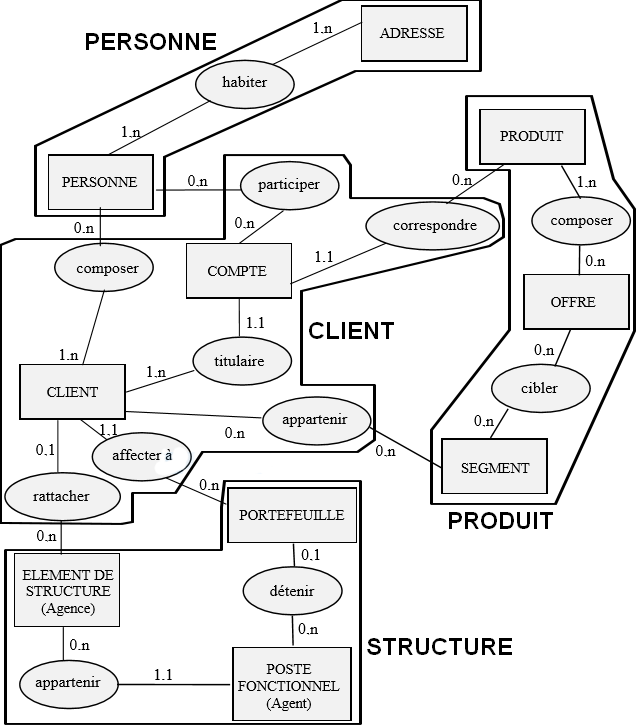
\includegraphics[width=\textwidth]{figures/mcd/MCD_Clients_Produits}
\caption{MCD Clients Produits}
\end{figure}


\section{Données commerciales}
\begin{figure}[H]
\centering
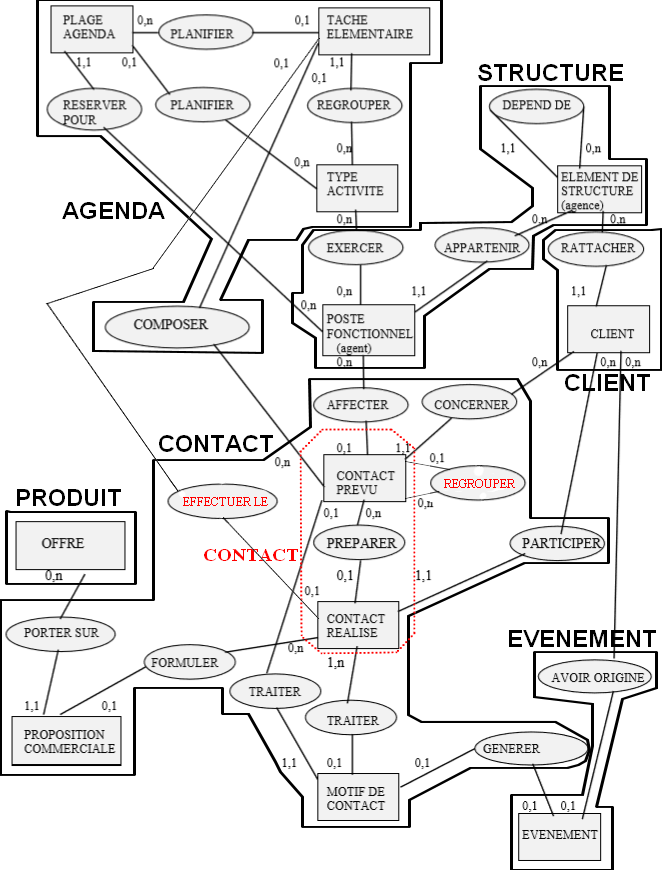
\includegraphics[width=\textwidth]{figures/mcd/MCD_Commercial}
\caption{MCD Commercial}
\end{figure}
\section{Diagramme d’état de l'objet métier 'contacts'}
\begin{figure}[H]
\centering
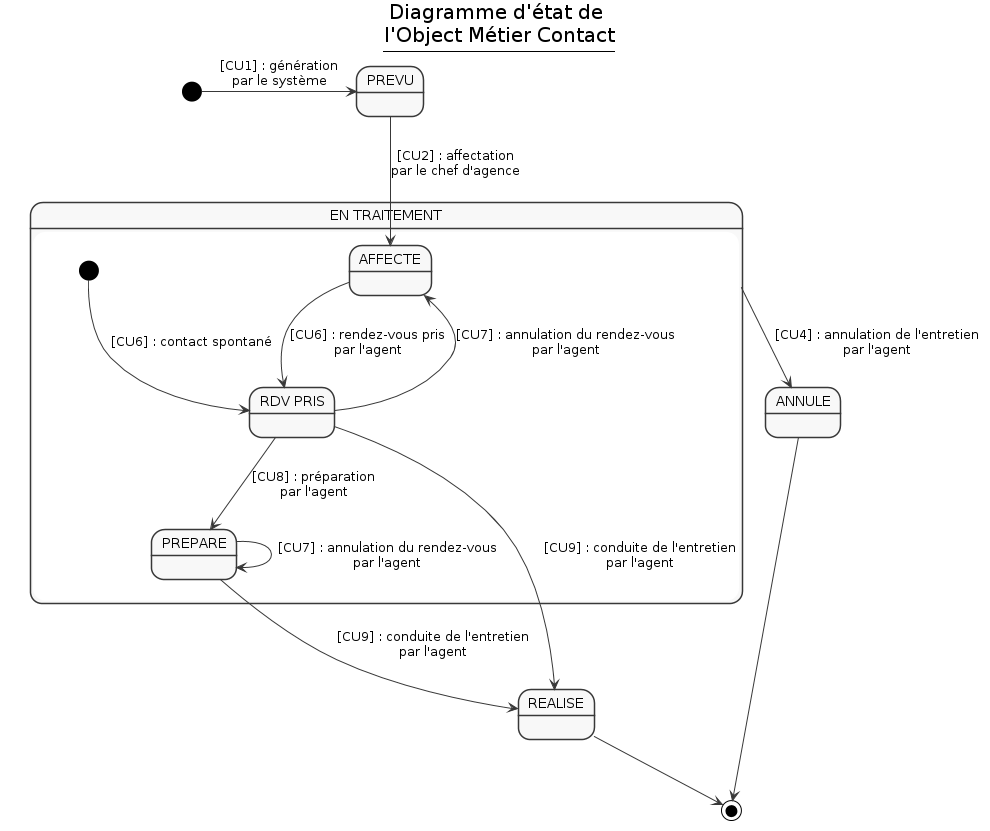
\includegraphics[width=\textwidth]{figures/diag_etats_contact}
\caption{Diagramme d'état de l'objet métier contact}
\end{figure}



\section{Architecture technique}

\todo{Relire l'intégralité de cette section}

Cette section présente les choix techniques effectués dans le cadre de la conception de l'architecture technique.

\subsection{Choix du type d'IHM}

Nous avons choisi de concevoir un client léger sous forme d'une application web. Nous avons réalisé ce choix après considération de différents critères. Il nous semble plus facile de maintenir une application centralisée putôt qu'une application distribuée. En effet, dès qu'une mise à jour de l'application est réalisée, il est plus simple de mettre à jour l'application sur un serveur que sur plusieurs centaines de postes clients. Cette application ne pouvant être utilisée hors ligne, un client lourd ne présente pas plus d'intérêt selon ce critère. Il est également important de considérer le fait que le client lourd implique une grande quantité de travail pour l'adapter à des environnements différents tandis qu'un simple navigateur à jour permettra d'accèder à l'application. En effet, même si ce client lourd est développé dans un langage permettant la portabilité du code, il nécessitera l'installation de dépendances pour son fonctionnement ce qui n'est pas viable à long terme et implique des coûts important en terme de ressources. 

\subsection{Serveurs et localisation}

La répartition des serveurs présentée dans la suite fait référence à la figure suivante présentant le diagramme d'organisation fourni dans le sujet.

\begin{figure}[H]
    \centering
	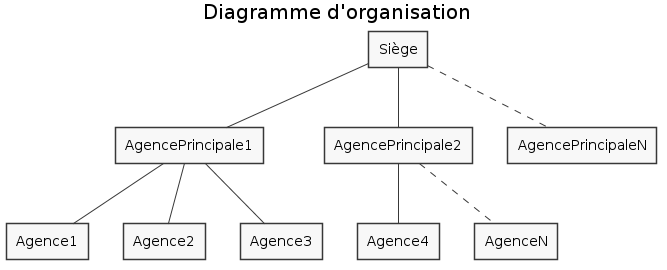
\includegraphics[scale=0.6]{figures/DO.png}
	\caption{Diagramme d'organisation}
\end{figure}

Nous avons répartis les serveurs de données en répondant aux questions suivantes :\\
\begin{itemize}
	\item[\textbullet] La donnée est-elle partagée ? Si oui, par qui ?
	\item[\textbullet] Quelle est la fréquence d'accès à la donnée ?
	\item[\textbullet] En terme de sécurité, qui a besoin d'accéder à la donnée ?\\
\end{itemize}

Nous avons donc abouti à une répartition optimale selon nos critères. Des serveurs de données seront implantés au siège (site central) ainsi que dans les agences principales mais pas dans les agences rattachées aux agences principales. Etant donné le fait que la gestion des données clients et produits seront réalisées au siège, celui-ci nécessite évidemment des serveurs pour stocker ces données. Ensuite, il nous semble réaliste de distribuer la donnée propre à chaque agence au sein de l'angence principale à laquelle elle est rattachée. Cela permettra de ne pas surcharger d'information inutile les entités ne nécessitant pas l'accès à ces données. De plus, cela aura un effet important sur les performances globales du système et notamment la diminution du nombre de requêtes sur des sites distants qui aura pour effet de réduire le temps de réponse. Il nous semble par contre iréaliste de déployer un serveur de données par agence, ce qui entrainerait des coûts de maintenance non négligeables.\\

Nous avons procédé de la même manière concernant les serveurs d'applications avec des questions différentes :\\
\begin{itemize}
	\item[\textbullet] Est-il possible et intéressant, étant donnée la répartition des serveurs de données, de distribuer les composants applicatifs ?
	\item[\textbullet] Quelles seraient les conséquences d'un tel déploiement ?\\
\end{itemize}

Nous sommes donc arrivés aux conclusions suivantes. Afin de profiter des avantages offerts par le client léger, nous ne devons pas trop répartir les serveurs d'application et il n'est donc pas souhaitable d'équiper chaque agence d'un serveur d'applications. Il n'est pas non plus intéressant d'équiper seulement le siège d'un serveur d'application en particulier si l'on considère la charge qu'il subira si toutes les agences font appel à un serveur central. Il est également important de noter qu'en cas de disfonctionnement du serveur d'application sur le site central, toutes les agences seraient impactées. Il semble donc judicieux d'équiper chaque agence principale d'un serveur d'application. En effet, cela apporte de nombreux avantages. Parmis ceux-ci le fait de pouvoir déployer progressivement une nouvelle version d'un applicatif ce qui est pratiqué dans beaucoup de grand groupe avec des entités qui réalisent les tests des nouvelles versions sans impacter l'intégralité des agences jusqu'à la validation de la version. Cette répartition augmente également la tolérance aux pannes et la charge réseaux induite par les postes clients. Un serveur d'application devra tout de même être présent au siège pour supporter les composants applicatifs partagés.\\

Le tableau ci dessous présente la synthèse de nos choix concernant la répartition des serveurs et le nombre de serveurs à implanter. Ces choix seront renforcés par les choix concernant la répartition des blocs applicatifs et les flux de données induits par cette architecture. 


\begin{table}[H]
    \centering
    \begin{tabular}{l|l|l}
    Type d'entité        & Serveur de Données & Serveur d'Applications \\ \hline
    Siège (site central) & Oui ($n$)            & Oui ($n$)                \\
    Agence principale    & Oui ($1$)            & Oui ($1$)                \\
    Agence simple        & Non                & Non                    \\
    \end{tabular}
    \caption{Tableau de répartition des serveurs par entité organisationnelle}
\end{table}

La figure suivante présente la répartition des serveurs.

\begin{figure}[H]
    \centering
    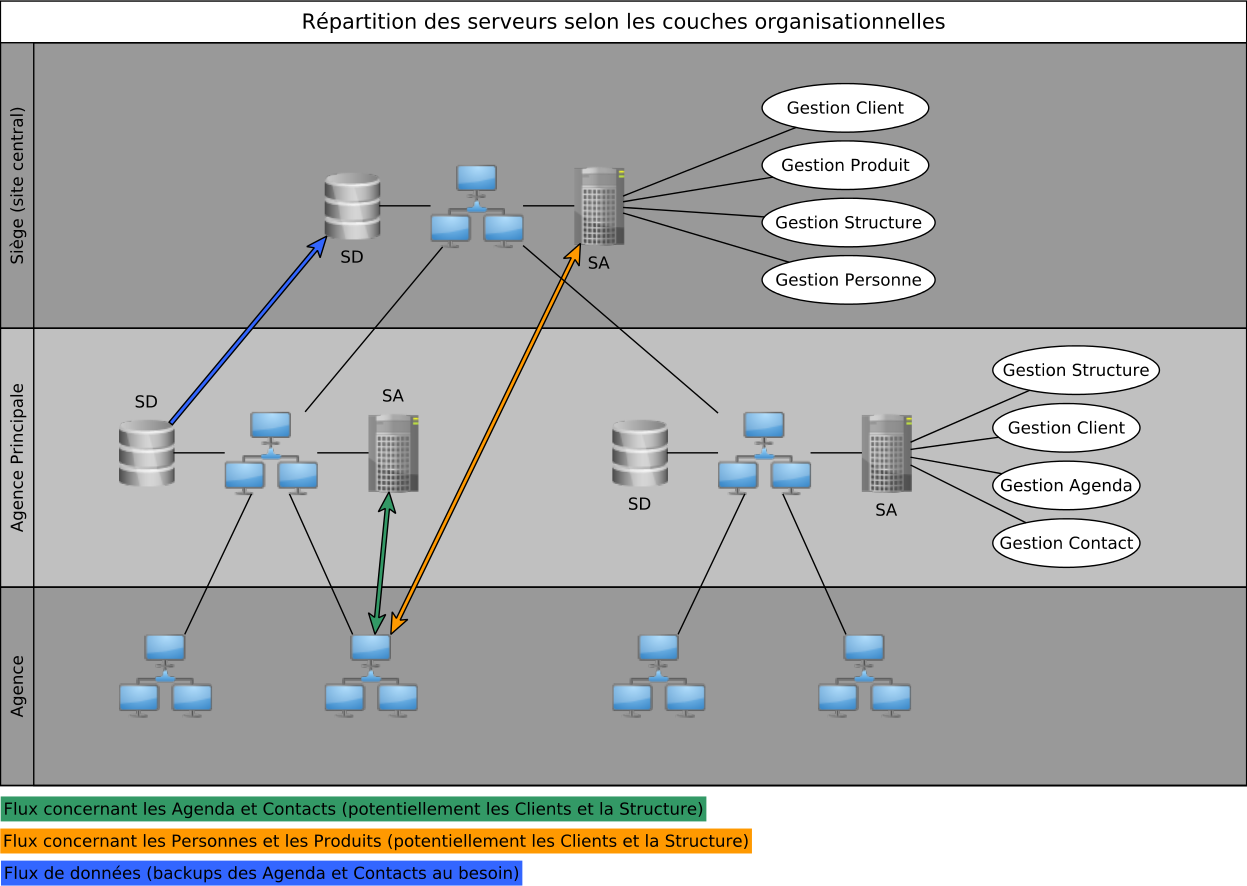
\includegraphics[scale=0.5]{figures/architectureServeurs.png}
    \caption{Plan de répartition des serveurs}
\end{figure}

\subsection{Implantation des composants du noyau applicatif et flux de données}

Etant donnée la répartition des serveurs précédemment exposée et la contrainte concernant la gestion des données client et produit nous avons jugé qu'il serait intéressant de déployer les blocs applicatifs Personne, Client, Produit et Structure sur le(s) serveur(s) d'applications situé(s) sur le site central c'est-à-dire au siège. Il semble également envisageable de distribuer les composants Contact et Agenda sur les serveurs d'applications respectifs des différentes agences principales. Il pourrait être avantageux de répliquer les données concernant les client et les structures au niveau des agences principales. \\

Si nous considérons les flux de données, relatifs à des opérations classiques, induits par ces différents choix nous obtenons les résultats suivants. Une opération de consultation ou d'édition de l'agenda ne ferait intervenir que les serveurs situés au niveau de l'agence. Seules les opérations de consultation d'un client ou d'un produit feront intervenir les serveurs du site central. Enfin, la réplication des clients concernant une agence rattachée à une agence principale permettrait de gérer les évènement concernant les clients au niveau des agences principales également.
Du point de vue de la sécurité du système il est également intéressant de noter que la répartition choisie permet une bonne segmentation des données. Par exemple, la corruption d'un système au niveau d'une agence principale ne permettrait pas d'accèder aux agendas de toutes les agences ni à la liste de tous les clients. De même les informations confidentielles concernant les clients seront toutes stockées au siège ce qui permettra une protection efficace de ces dernières. Dans le cas d'une corruption de ce système central, l'attaquant ne sera pas forcément en mesure de consulter les agendas des agences. Cette architecture nécessite par contre des protections adéquates des communications entre les différents systèmes distribués.

\part{Conception fonctionnelle détaillée}
\setcounter{section}{0}

\section{CU1 - Génération de contacts}
\begin{figure}[H]
\centering
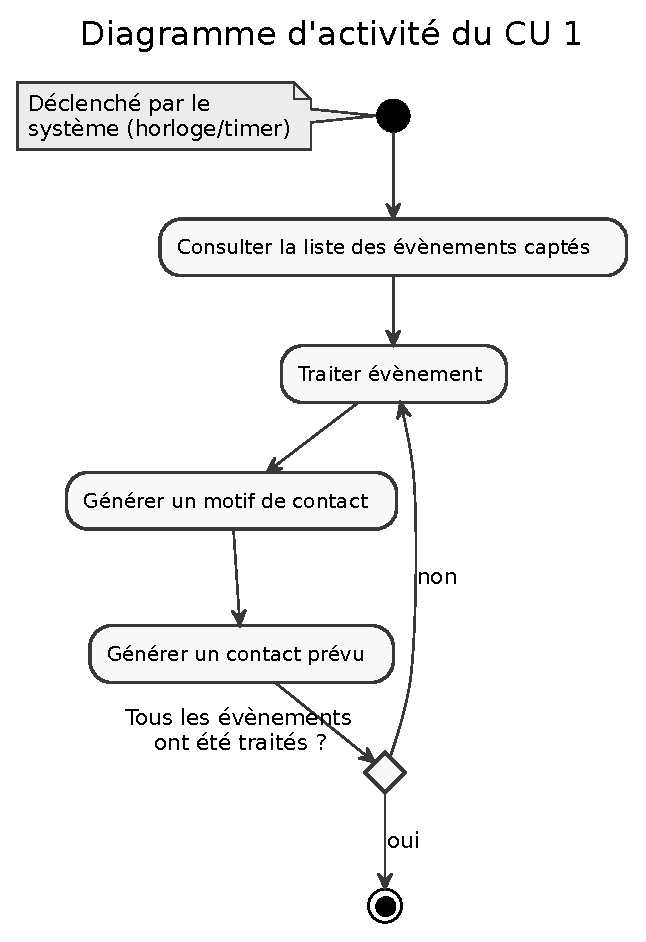
\includegraphics[width=10cm]{figures/eps/DA_CU1.eps}
\caption{DA du CU1}
\end{figure}

\begin{figure}[H]
\noindent\makebox[\textwidth]{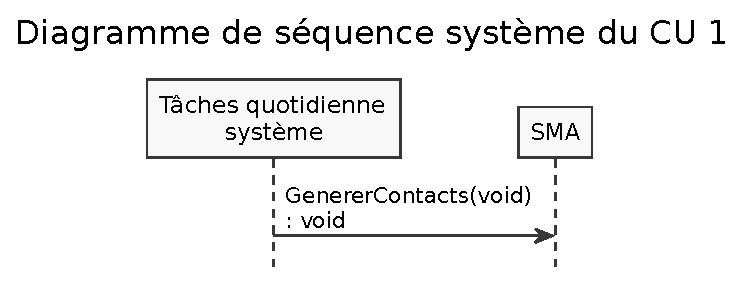
\includegraphics[width=19cm]{figures/eps/DSS_CU1.eps}}
\caption{DSS du CU1}
\end{figure}


\section{CU2 - Répartition des contacts commerciaux}

\begin{figure}[H]
\centering
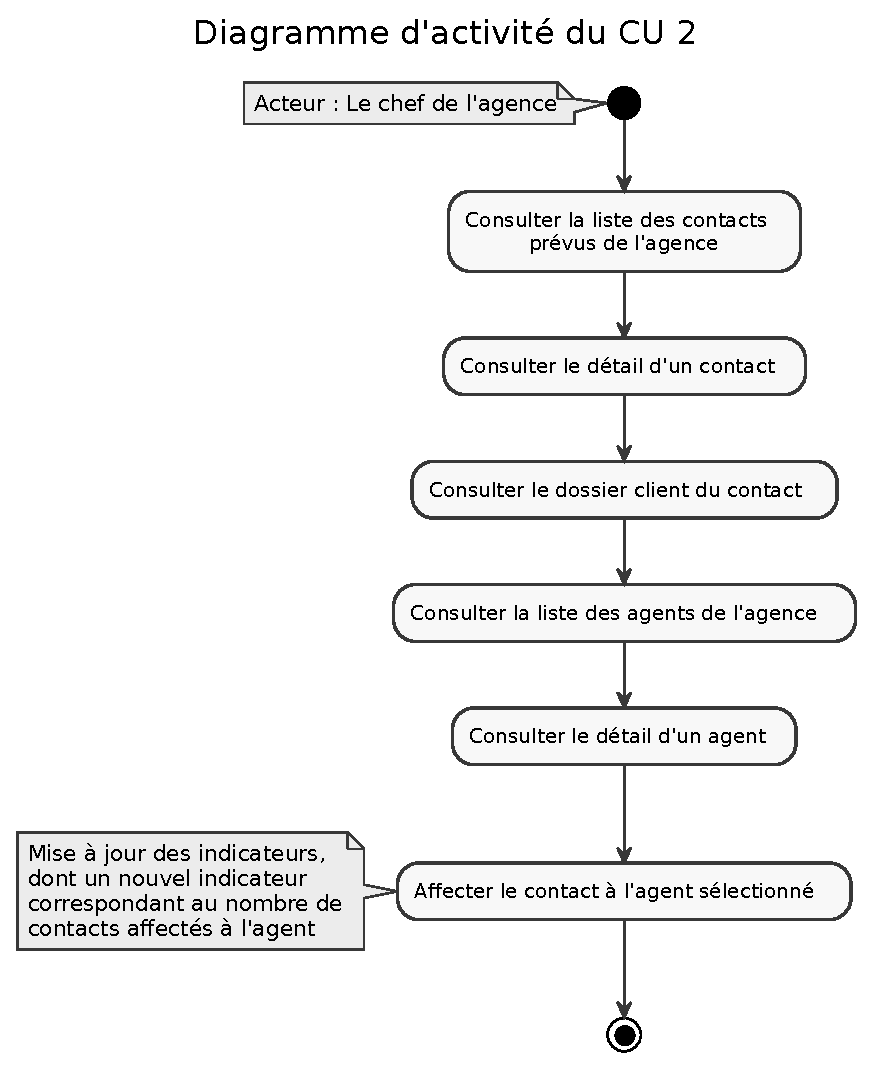
\includegraphics[width=\textwidth]{figures/eps/DA_CU2.eps}
\caption{DA du CU2}
\end{figure}


\begin{figure}[H]
\noindent\makebox[\textwidth]{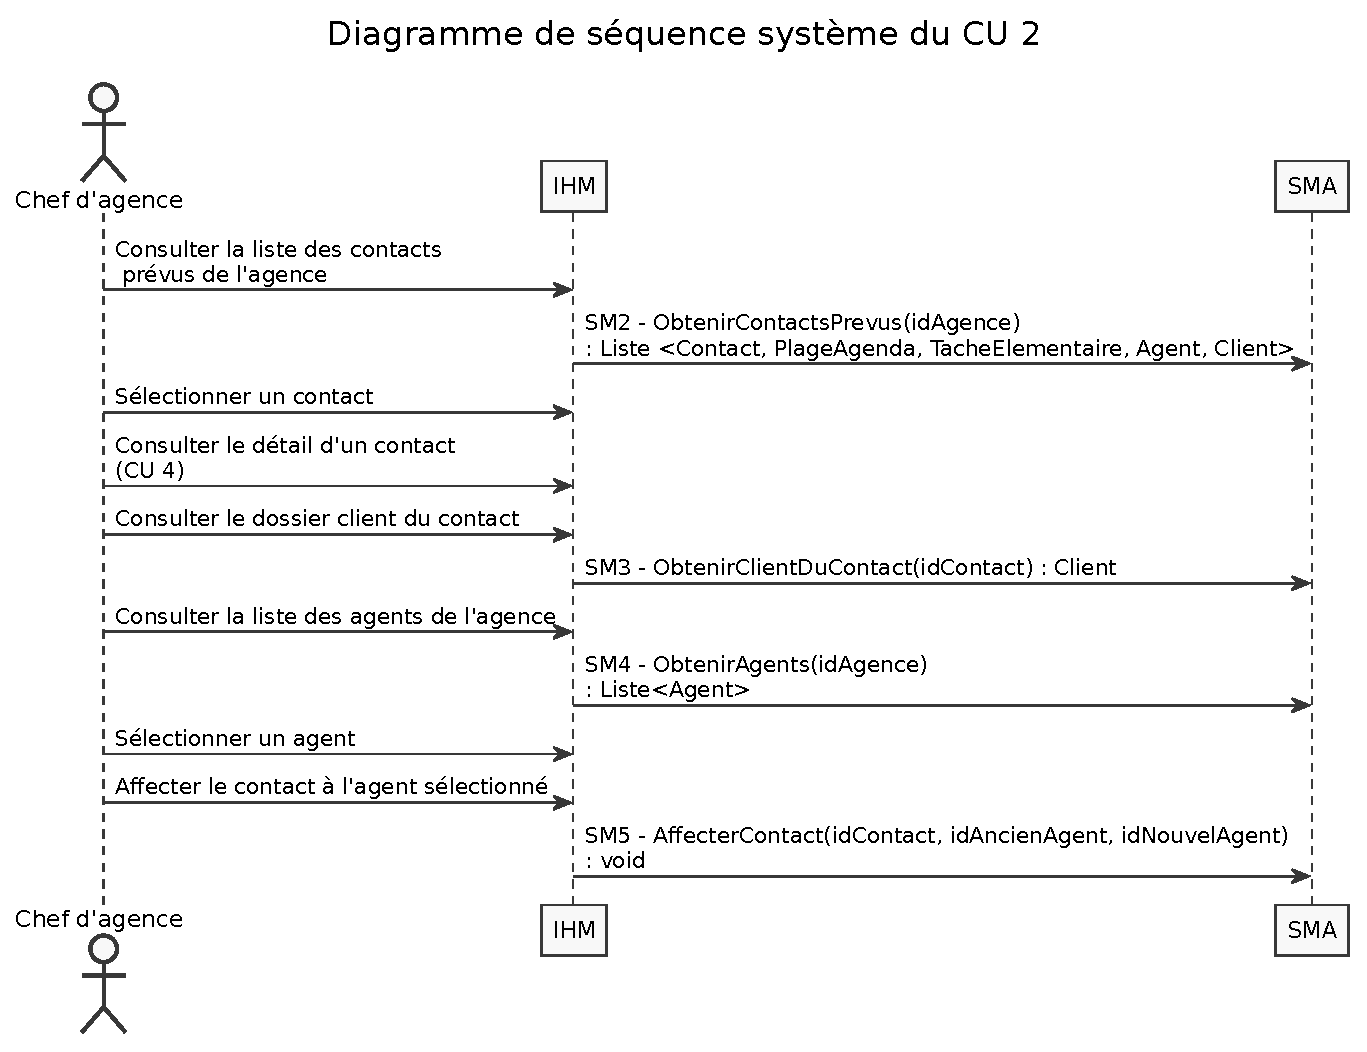
\includegraphics[width=19cm]{figures/eps/DSS_CU2.eps}}
\caption{DSS du CU2}
\end{figure}



\section{CU3 - Suivi de l’action commercial}

\begin{figure}[H]
\centering
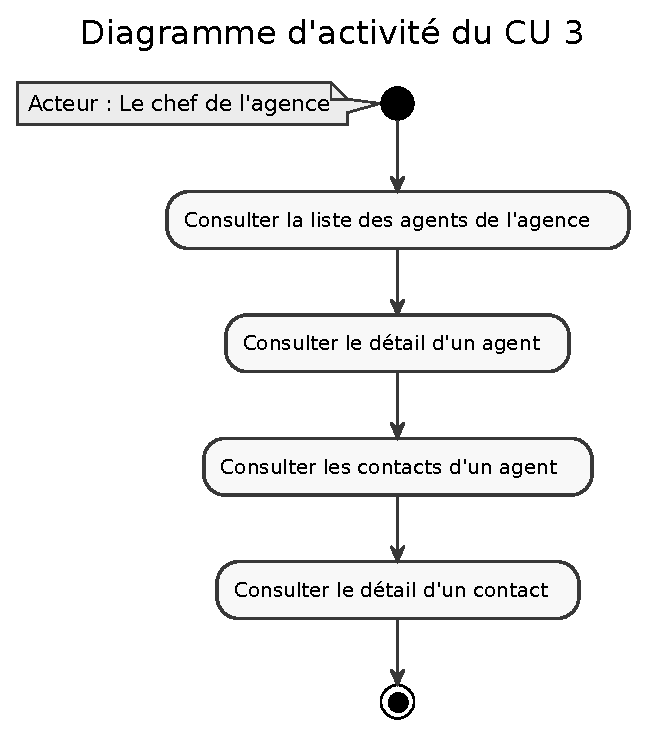
\includegraphics[width=10cm]{figures/eps/DA_CU3.eps}
\caption{DA du CU3}
\end{figure}

\begin{figure}[H]
\noindent\makebox[\textwidth]{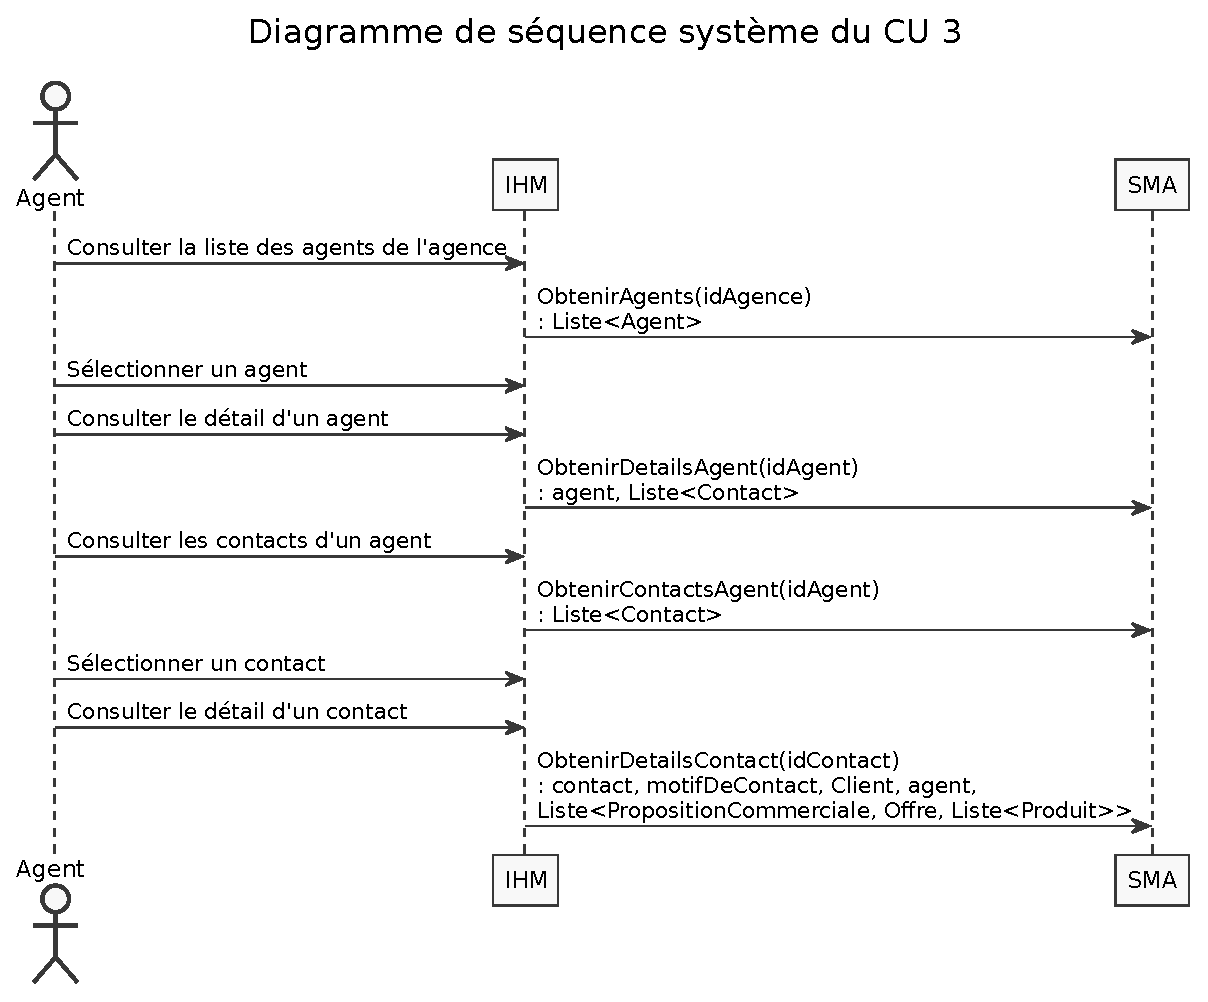
\includegraphics[width=19cm]{figures/eps/DSS_CU3.eps}}
\caption{DSS du CU3}
\end{figure}


\section{CU4 – Gestion de la liste des contacts clients}

\begin{figure}[H]
\noindent\makebox[\textwidth]{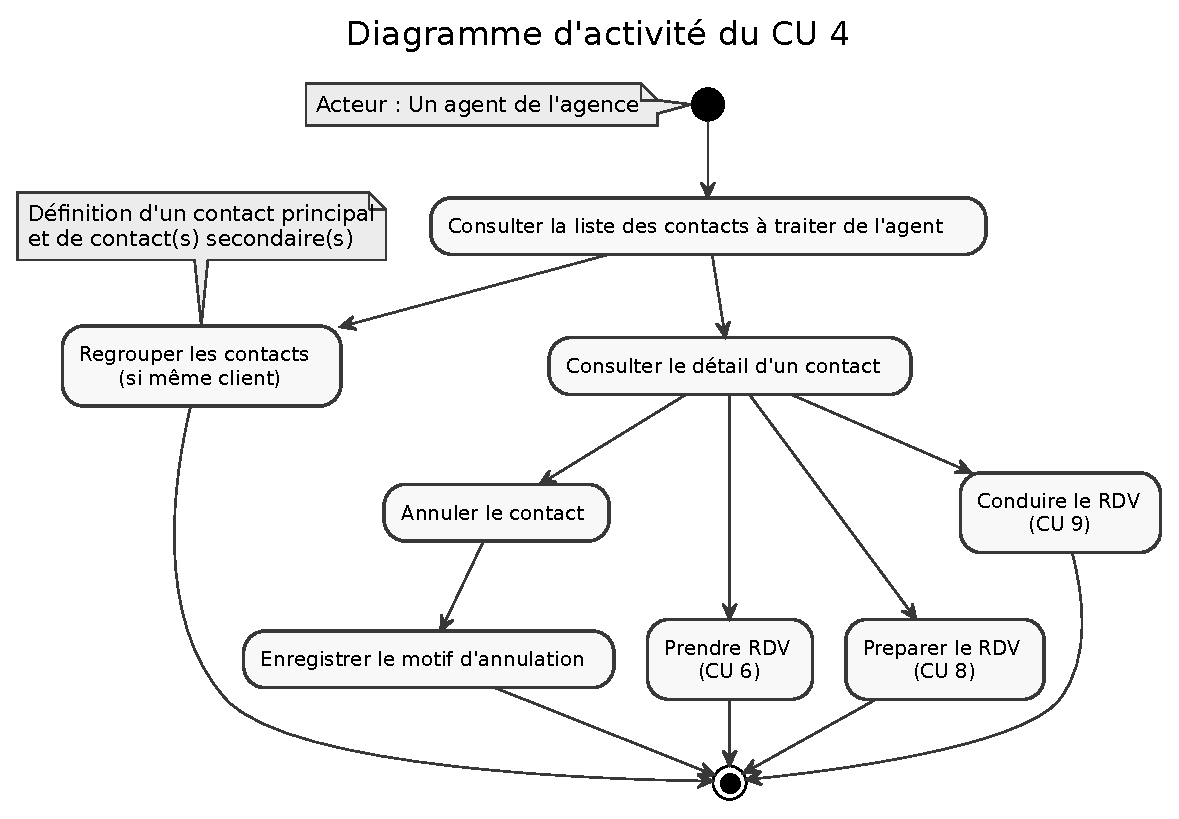
\includegraphics[width=19cm]{figures/eps/DA_CU4.eps}}
\caption{DA du CU4}
\end{figure}

\begin{figure}[H]
\noindent\makebox[\textwidth]{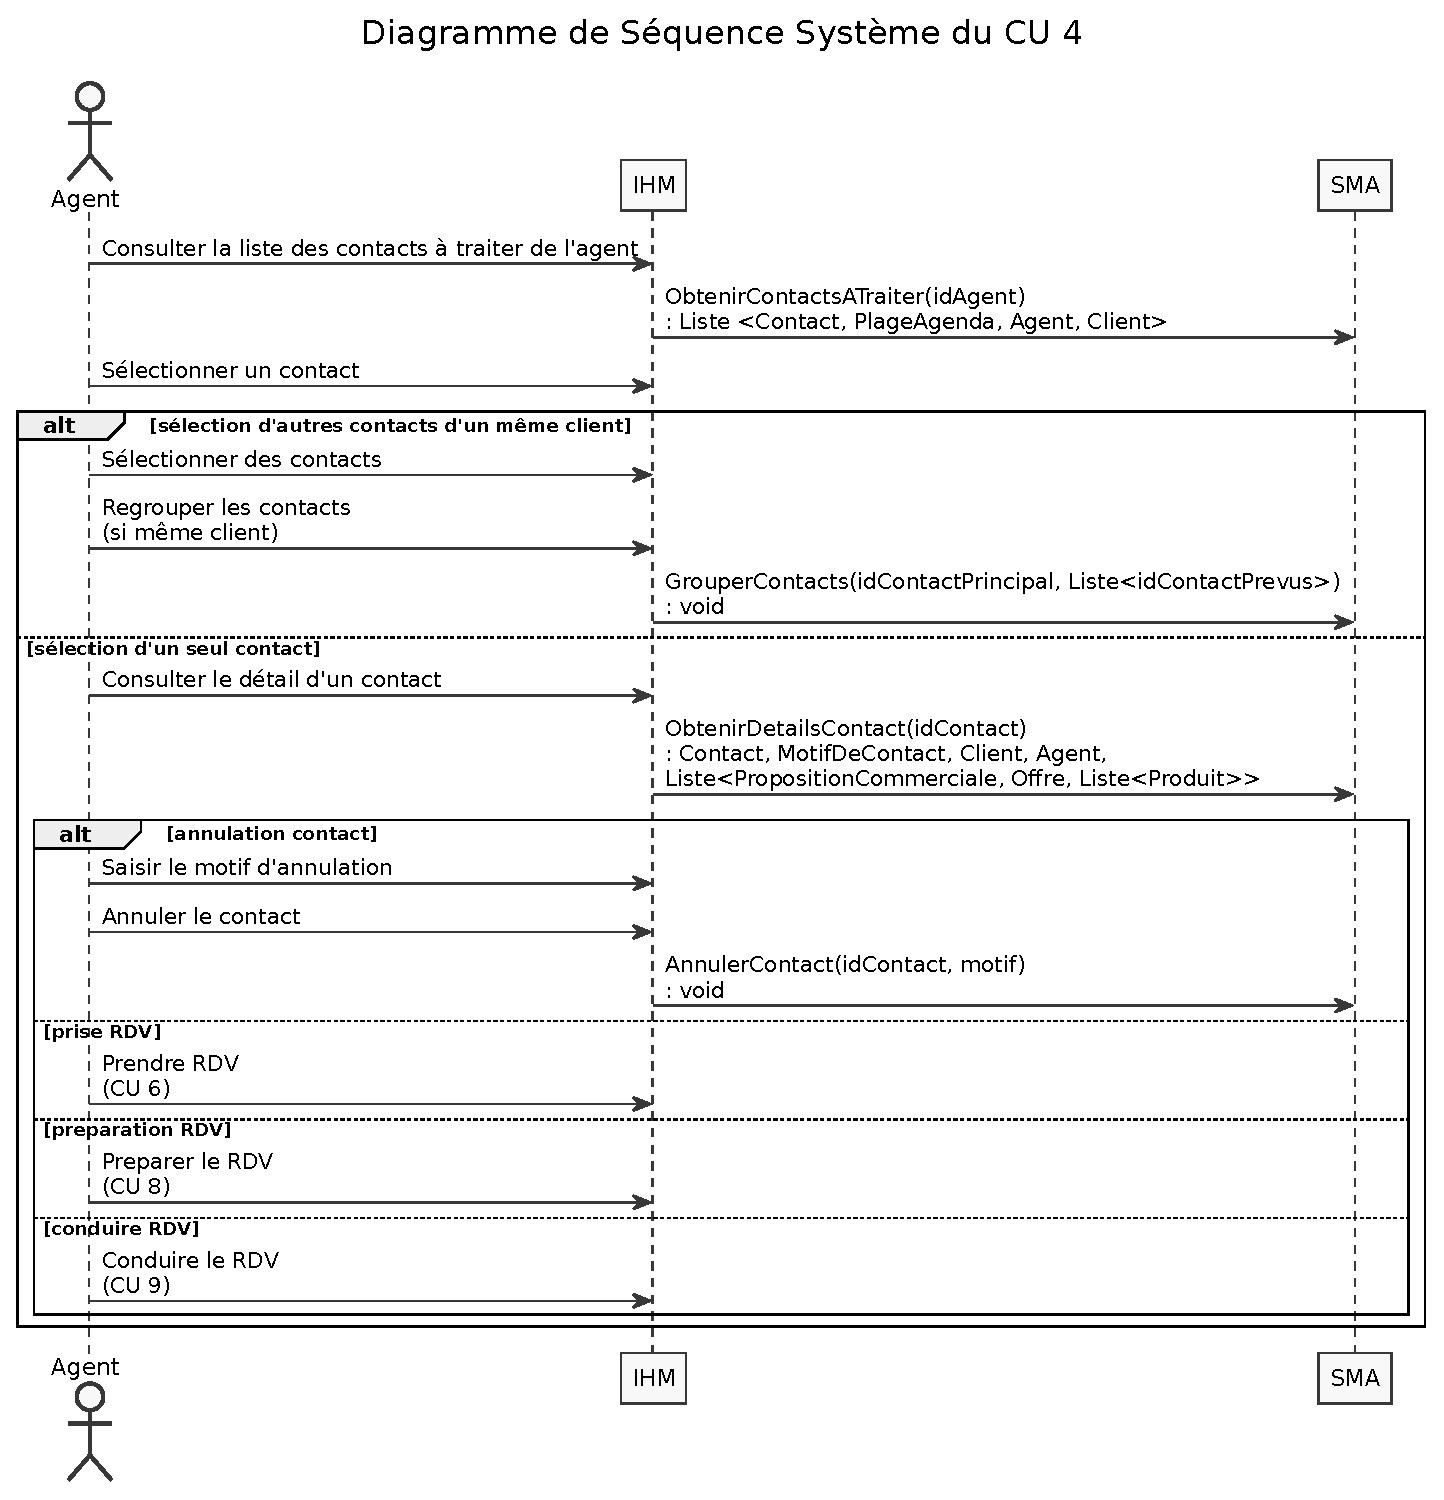
\includegraphics[width=19cm]{figures/eps/DSS_CU4.eps}}
\caption{DSS du CU4}
\end{figure}




\section{CU5 - Planification de l’activité de l’agence du mois suivant}

\begin{figure}[H]
\centering
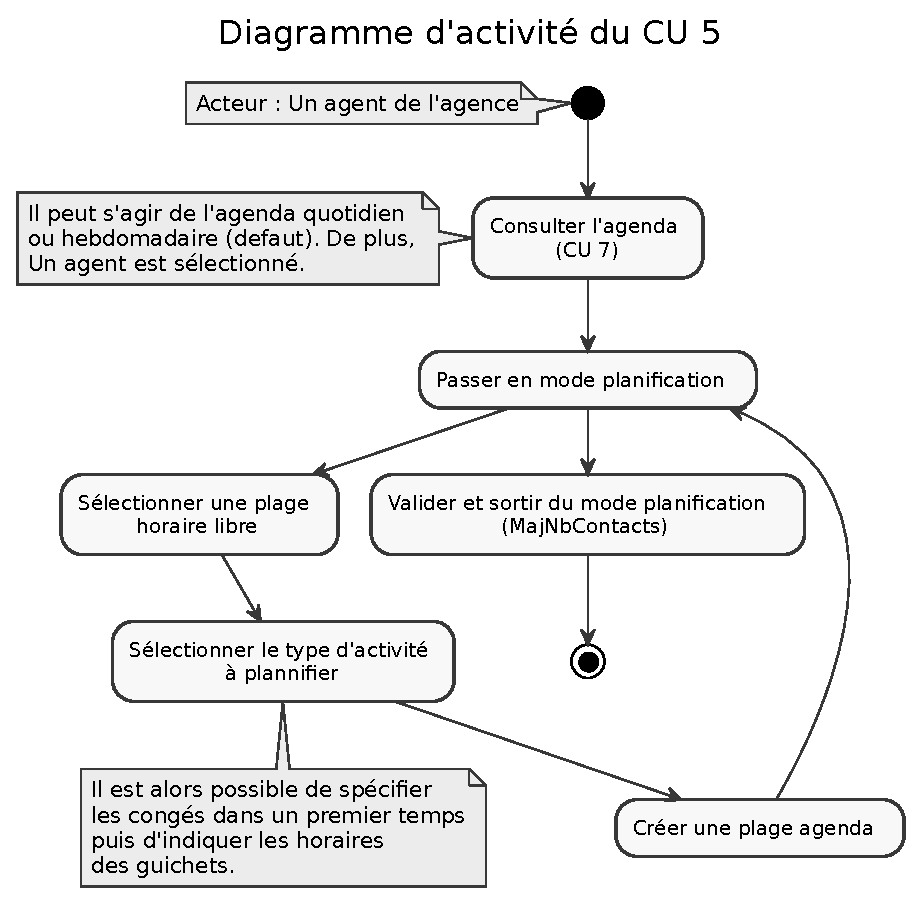
\includegraphics[width=\textwidth]{figures/eps/DA_CU5.eps}
\caption{DA du CU5}
\end{figure}

\begin{figure}[H]
\noindent\makebox[\textwidth]{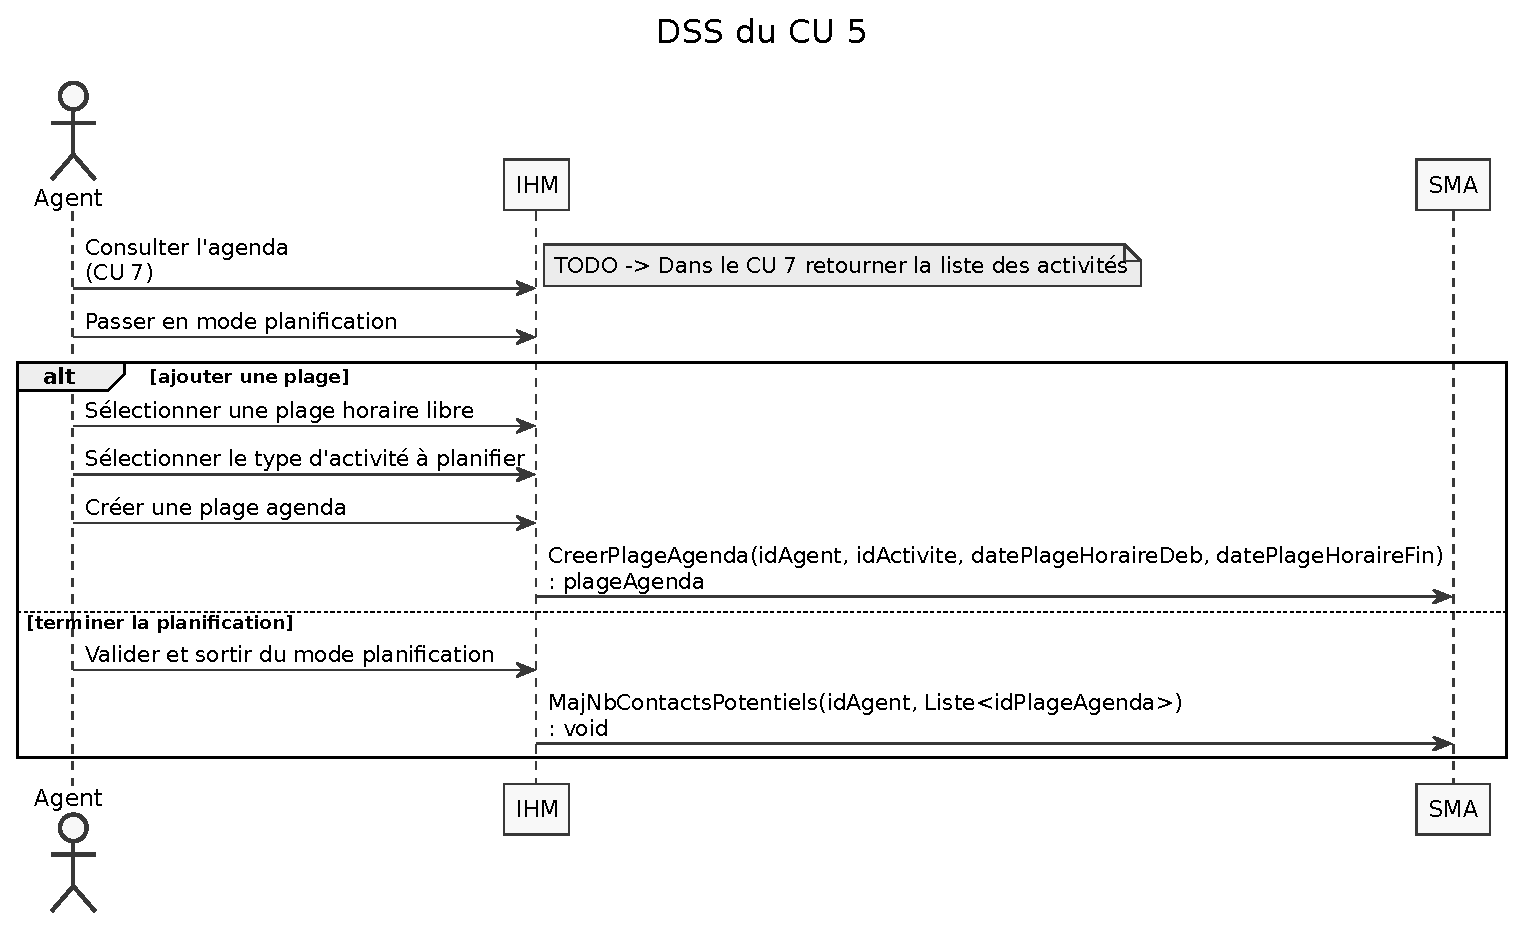
\includegraphics[width=19cm]{figures/eps/DSS_CU5.eps}}
\caption{DSS du CU5}
\end{figure}


\section{CU6 - Planification des contacts commerciaux}

\subsection{Partie Agent}
\begin{figure}[H]
\centering
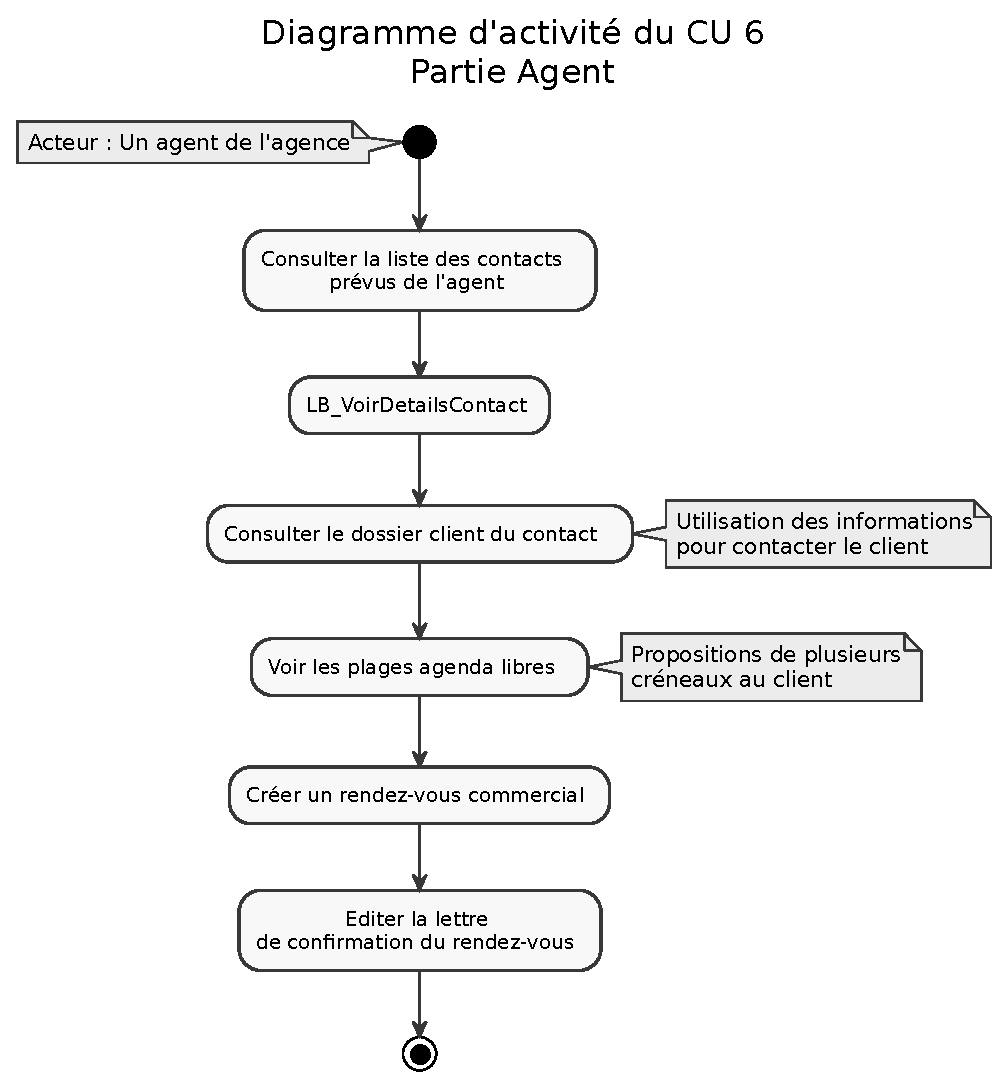
\includegraphics[width=\textwidth]{figures/eps/DA_CU6_partieAgent.eps}
\caption{DA du CU6}
\end{figure}

\begin{figure}[H]
\noindent\makebox[\textwidth]{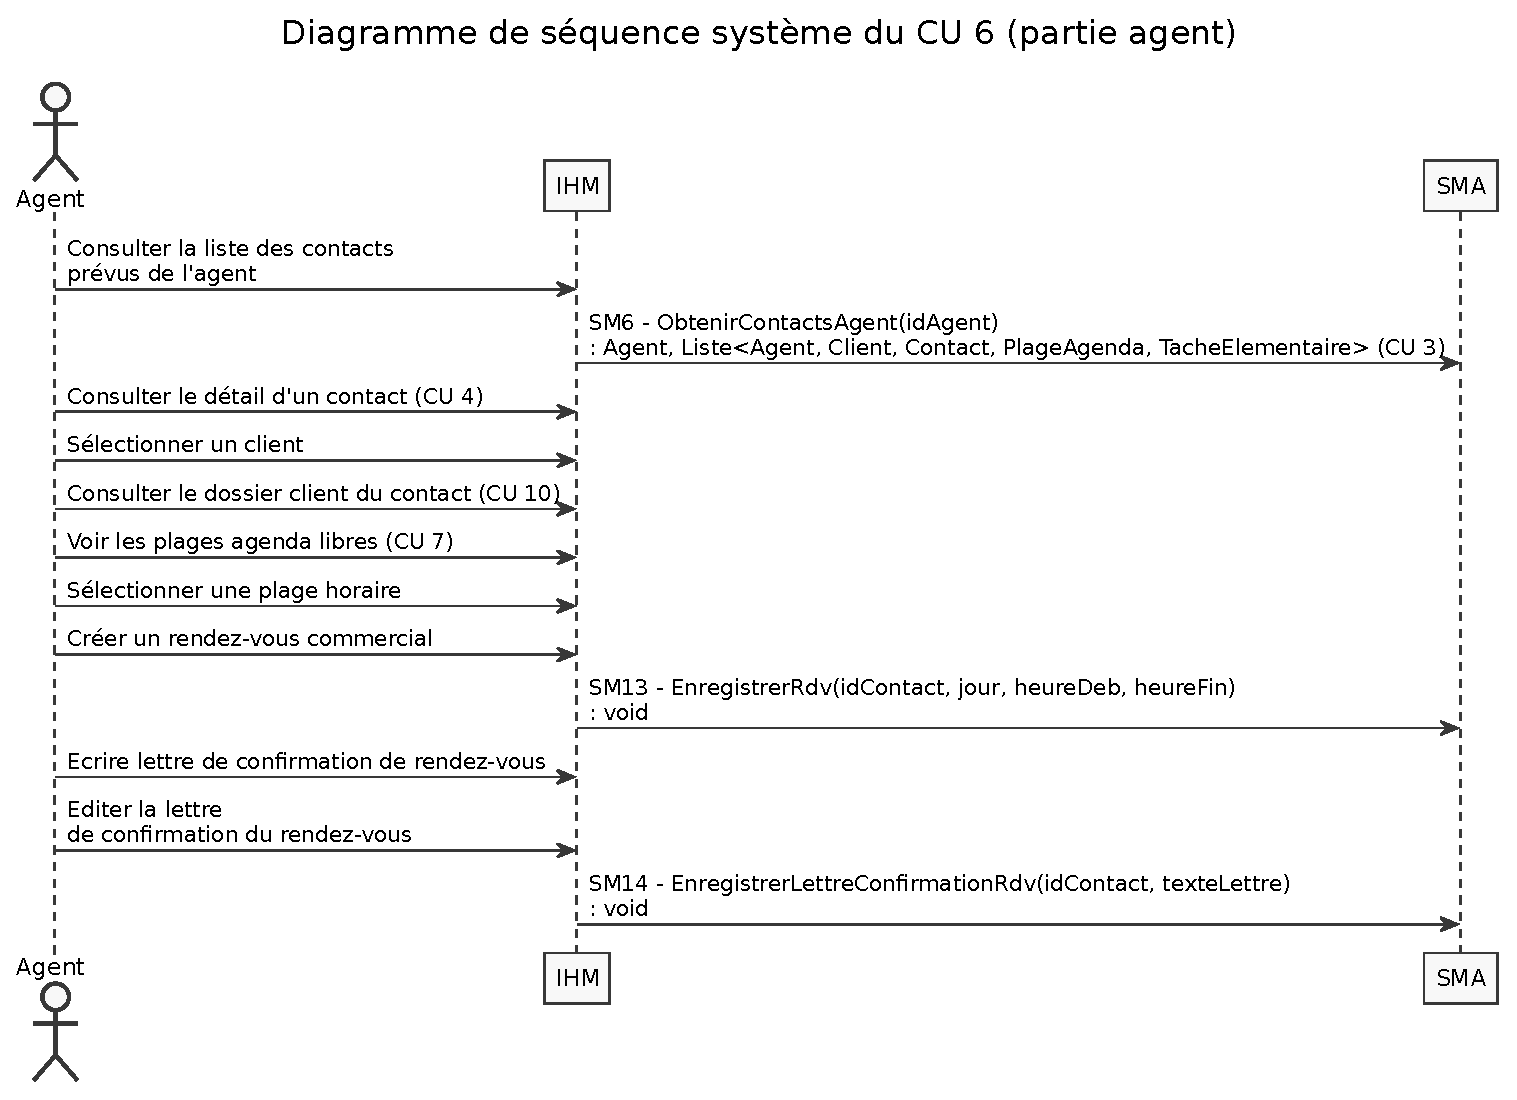
\includegraphics[width=19cm]{figures/eps/DSS_CU6_partieAgent.eps}}
\caption{DSS "contacts commerciaux" du CU6}
\end{figure}

\subsection{Partie Client}
\begin{figure}[H]
\centering
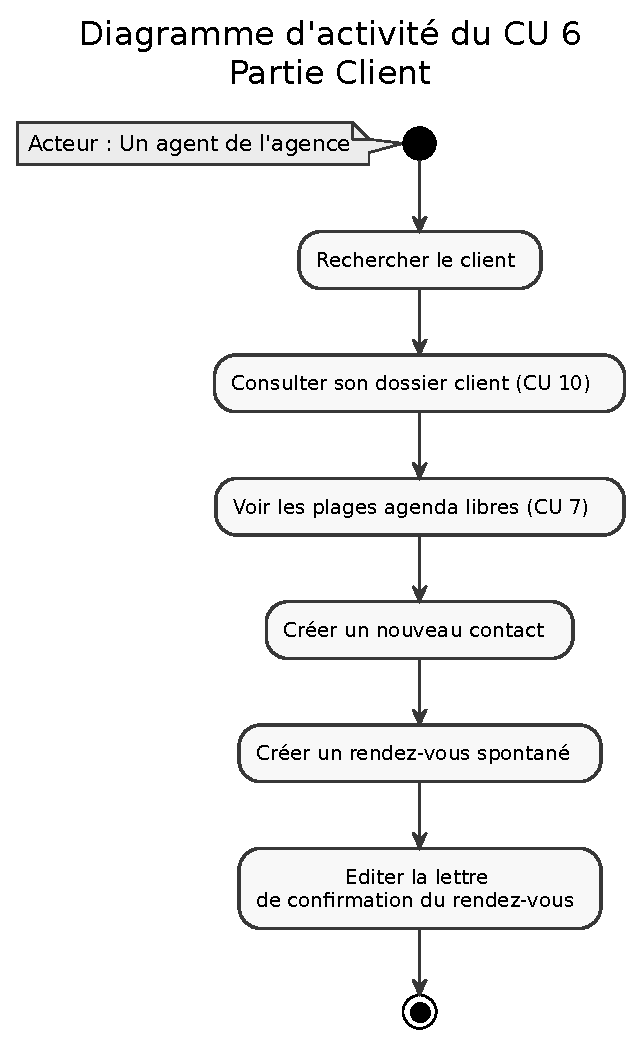
\includegraphics[width=10cm]{figures/eps/DA_CU6_partieClient.eps}
\caption{DA du CU6}
\end{figure}

\begin{figure}[H]
\noindent\makebox[\textwidth]{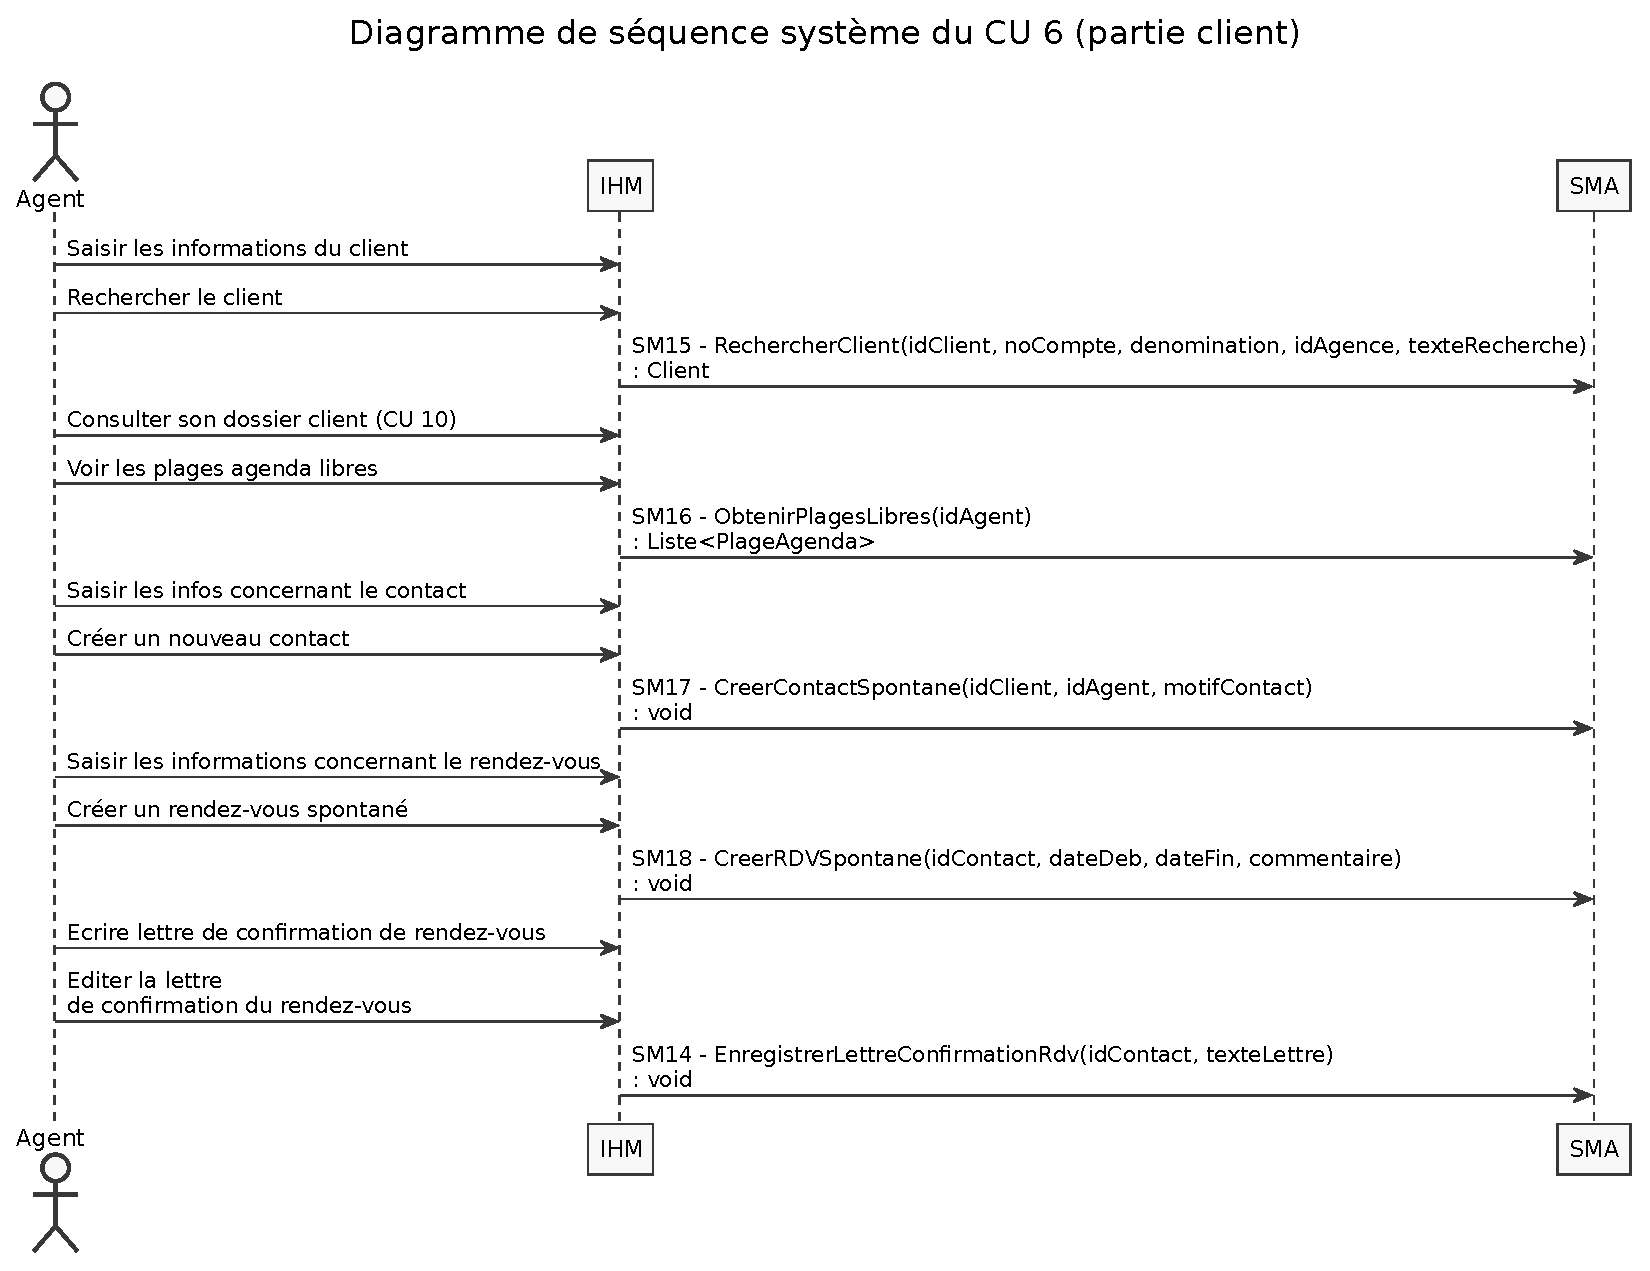
\includegraphics[width=19cm]{figures/eps/DSS_CU6_partieClient.eps}}
\caption{DSS "contacts spontanés" du CU6}
\end{figure}


\section{CU7 - Consultation des agendas}
\begin{figure}[H]
\centering
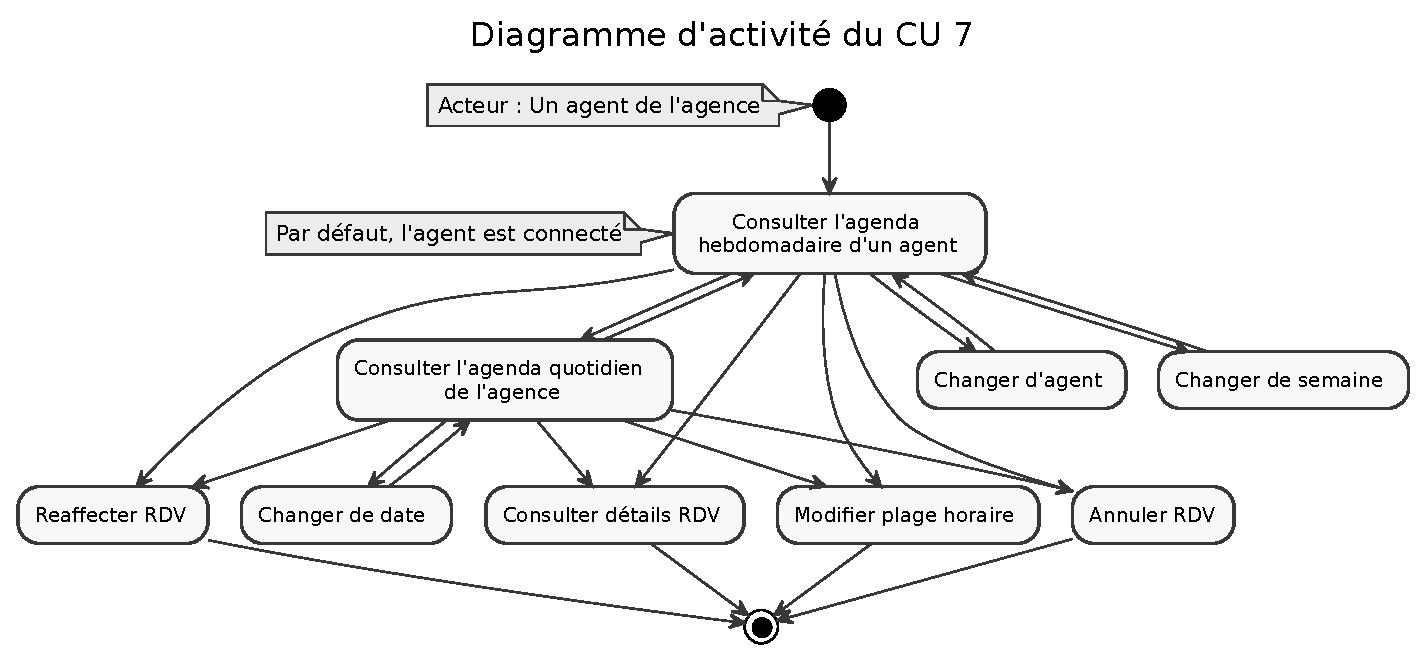
\includegraphics[width=20cm, angle=90]{figures/eps/DA_CU7.eps}
\caption{DA du CU7}
\end{figure}


\begin{figure}[H]
\noindent\makebox[\textwidth]{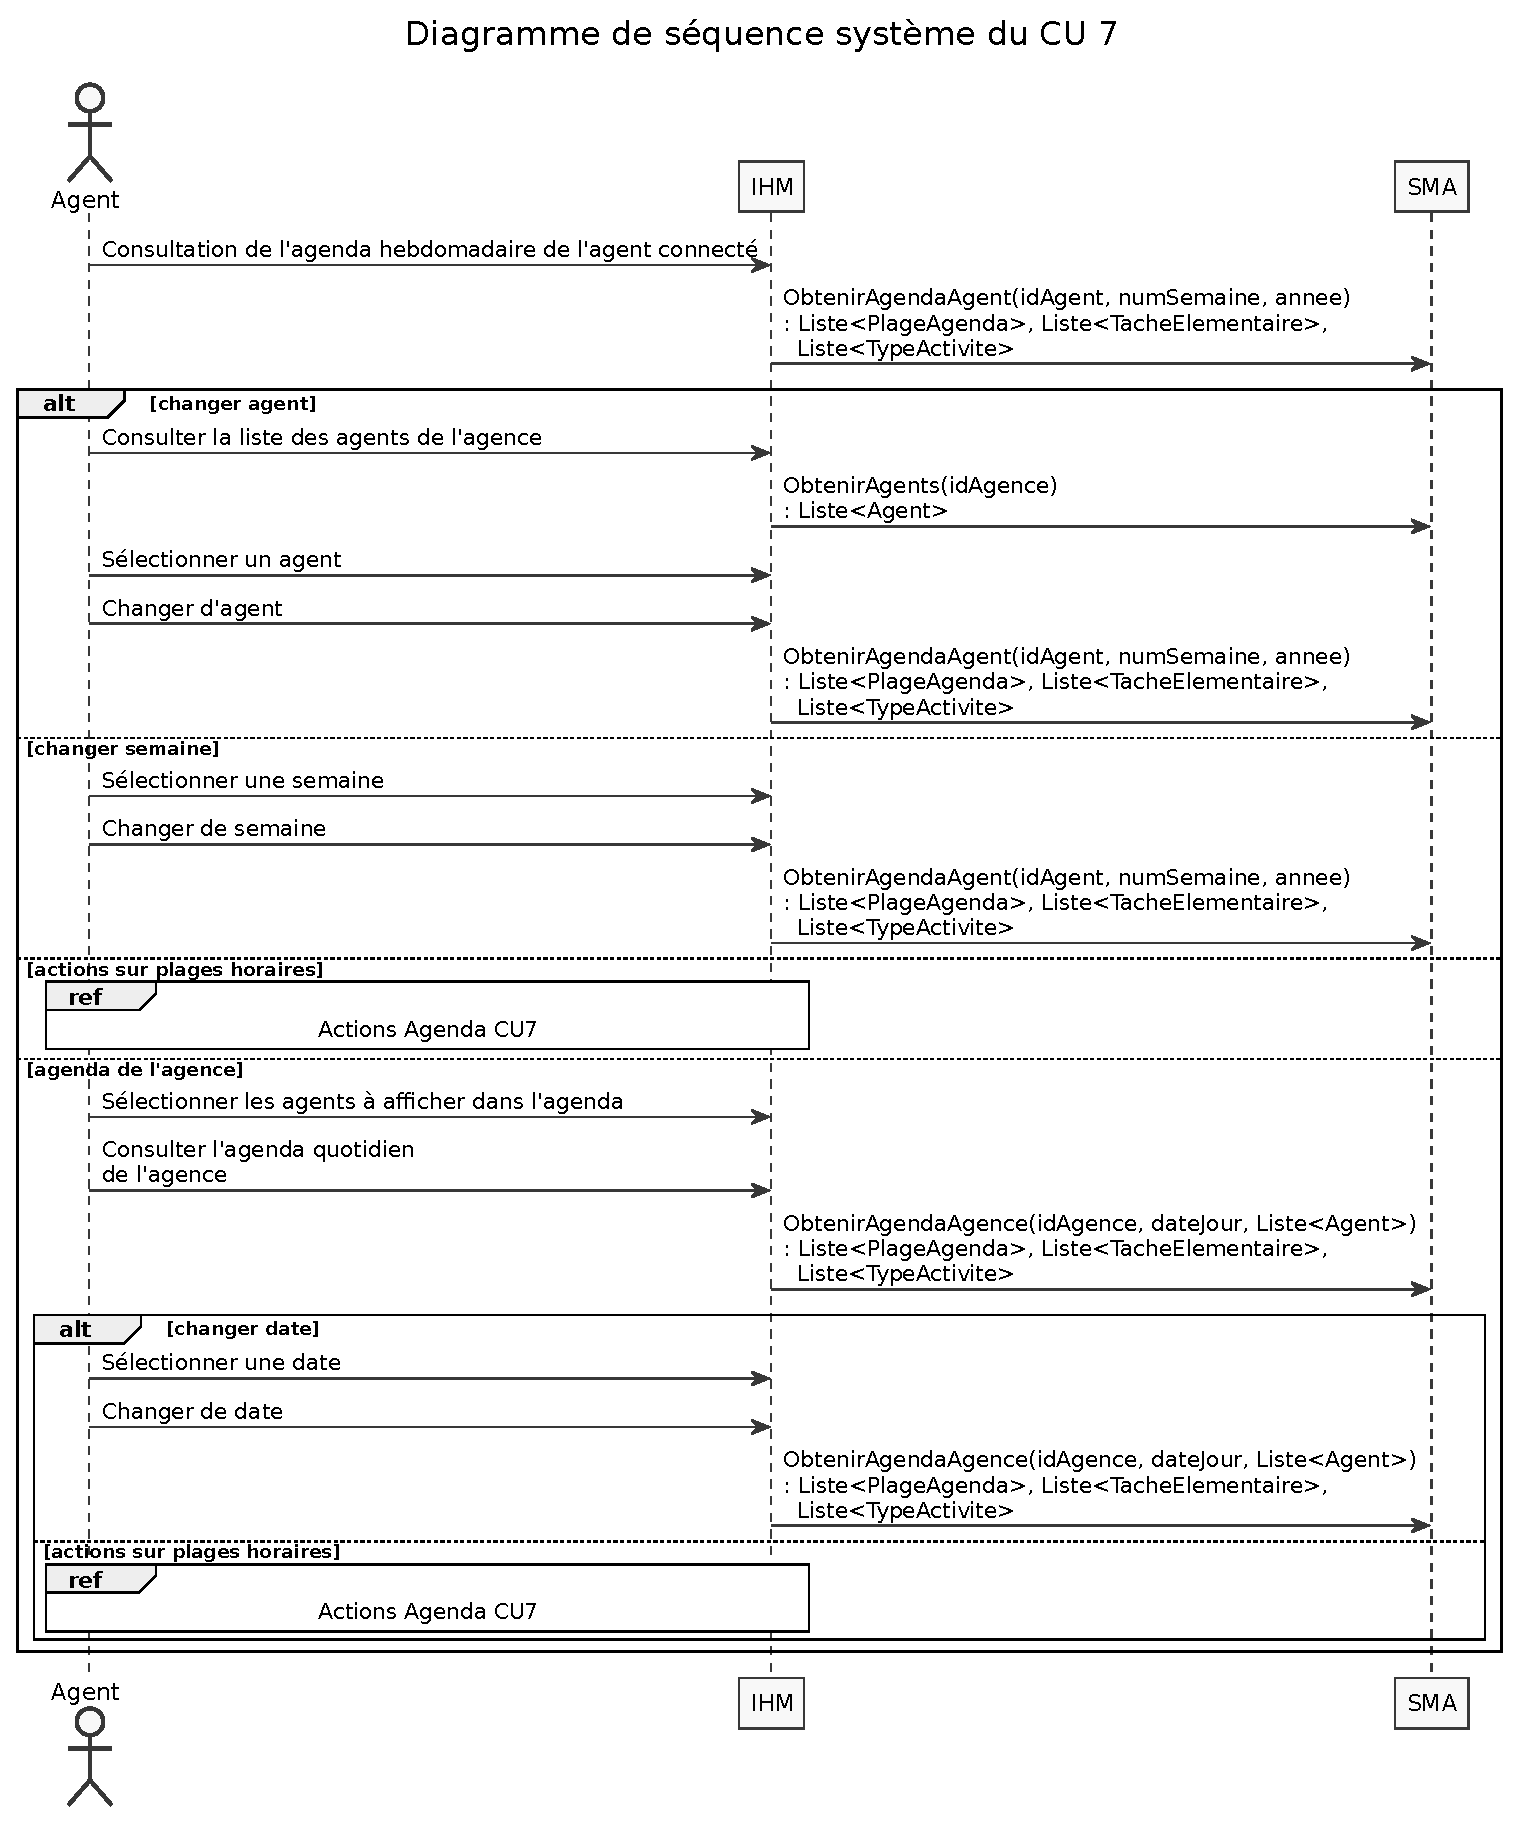
\includegraphics[width=19cm]{figures/eps/DSS_CU7.eps}}
\caption{DSS du CU7}
\end{figure}

\begin{figure}[H]
\noindent\makebox[\textwidth]{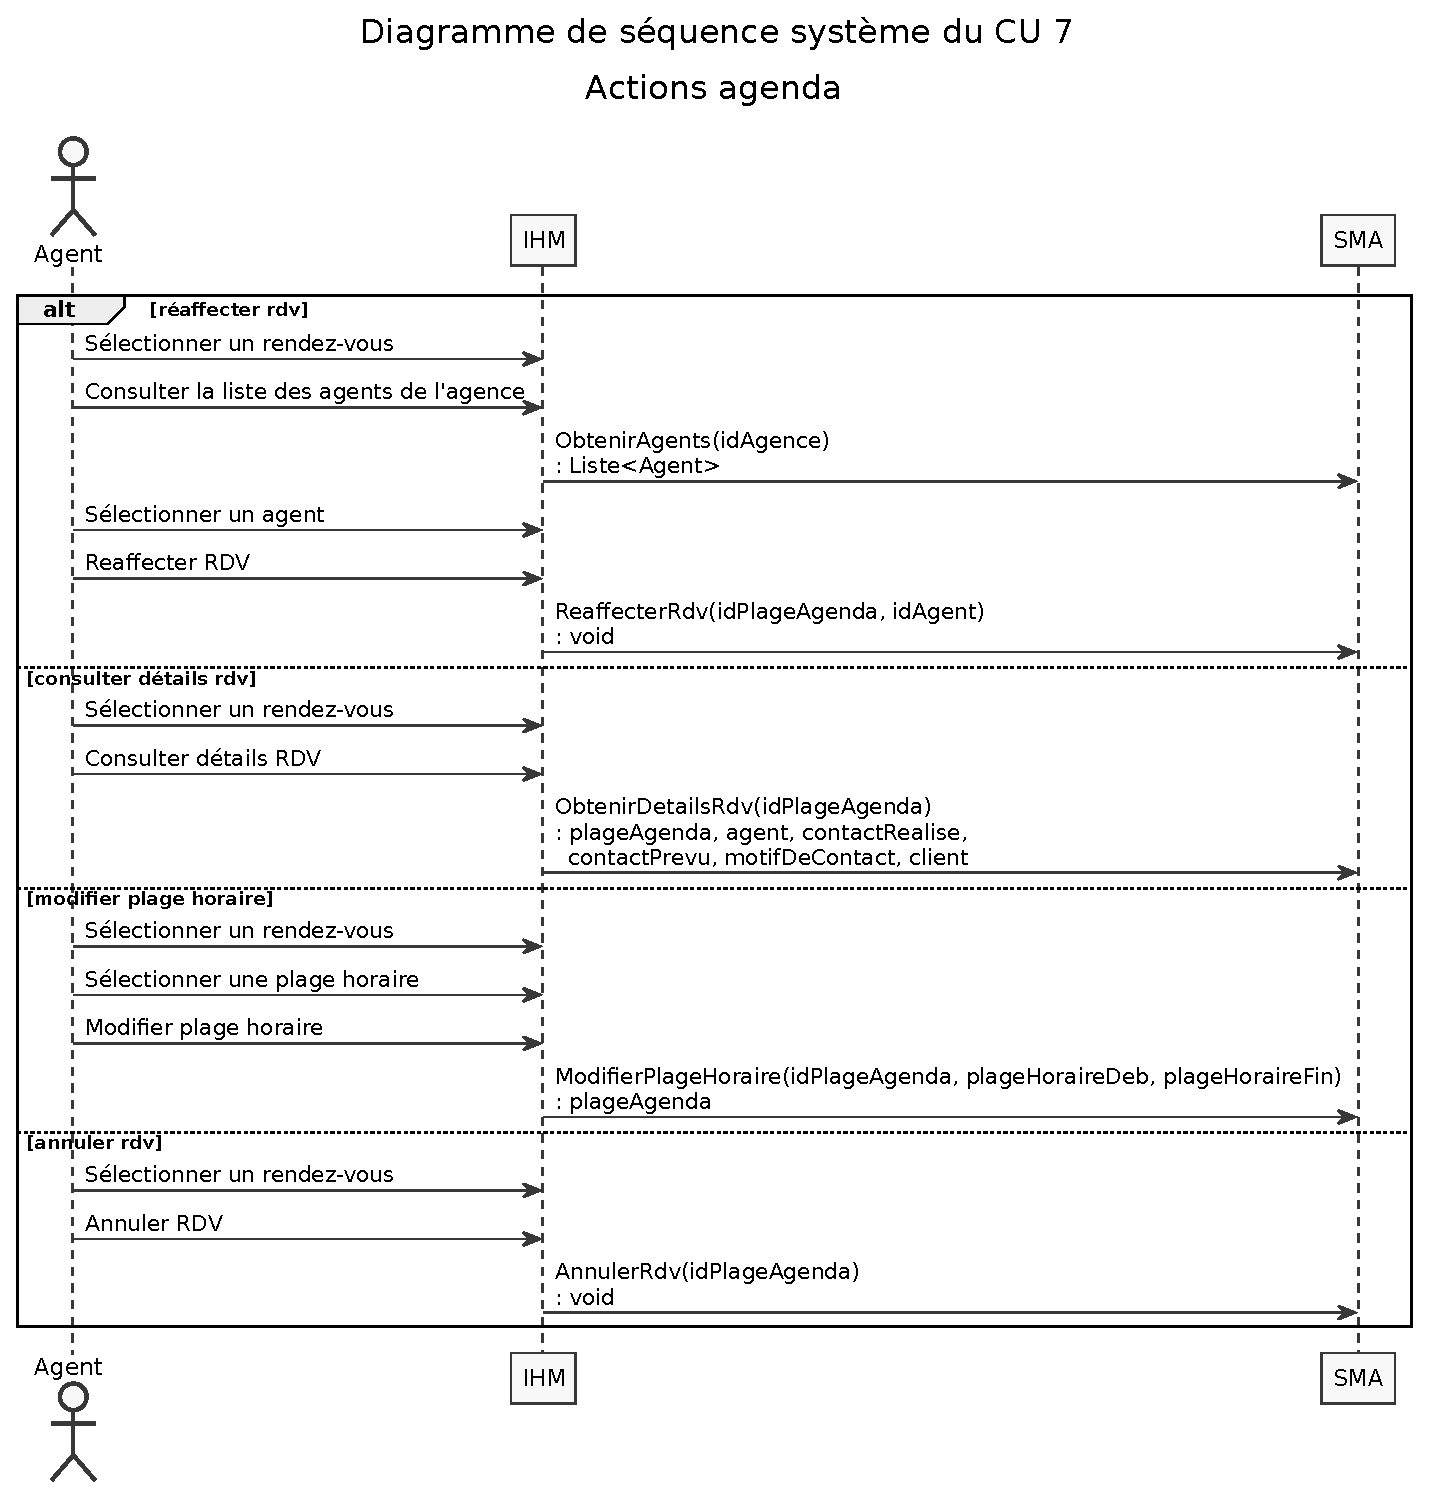
\includegraphics[width=19cm]{figures/eps/DSS_CU7_ActionsAgenda}}
\caption{DSS "Actions Agenda" du CU7}
\end{figure}

\section{CU8 - Préparation d’entretien par un agent}
\begin{figure}[H]
\centering
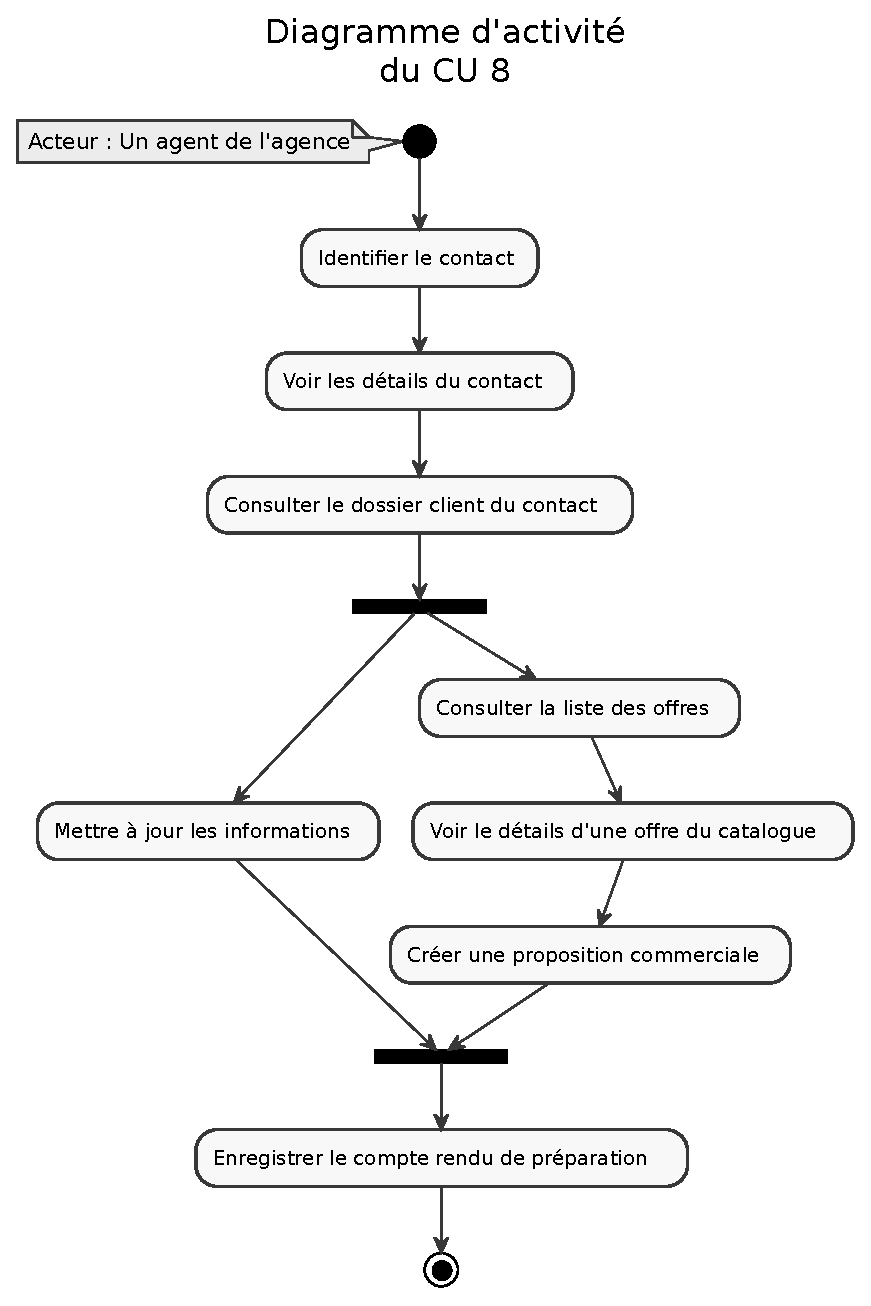
\includegraphics[width=\textwidth]{figures/eps/DA_CU8.eps}
\caption{DA du CU8}
\end{figure}

\begin{figure}[H]
\noindent\makebox[\textwidth]{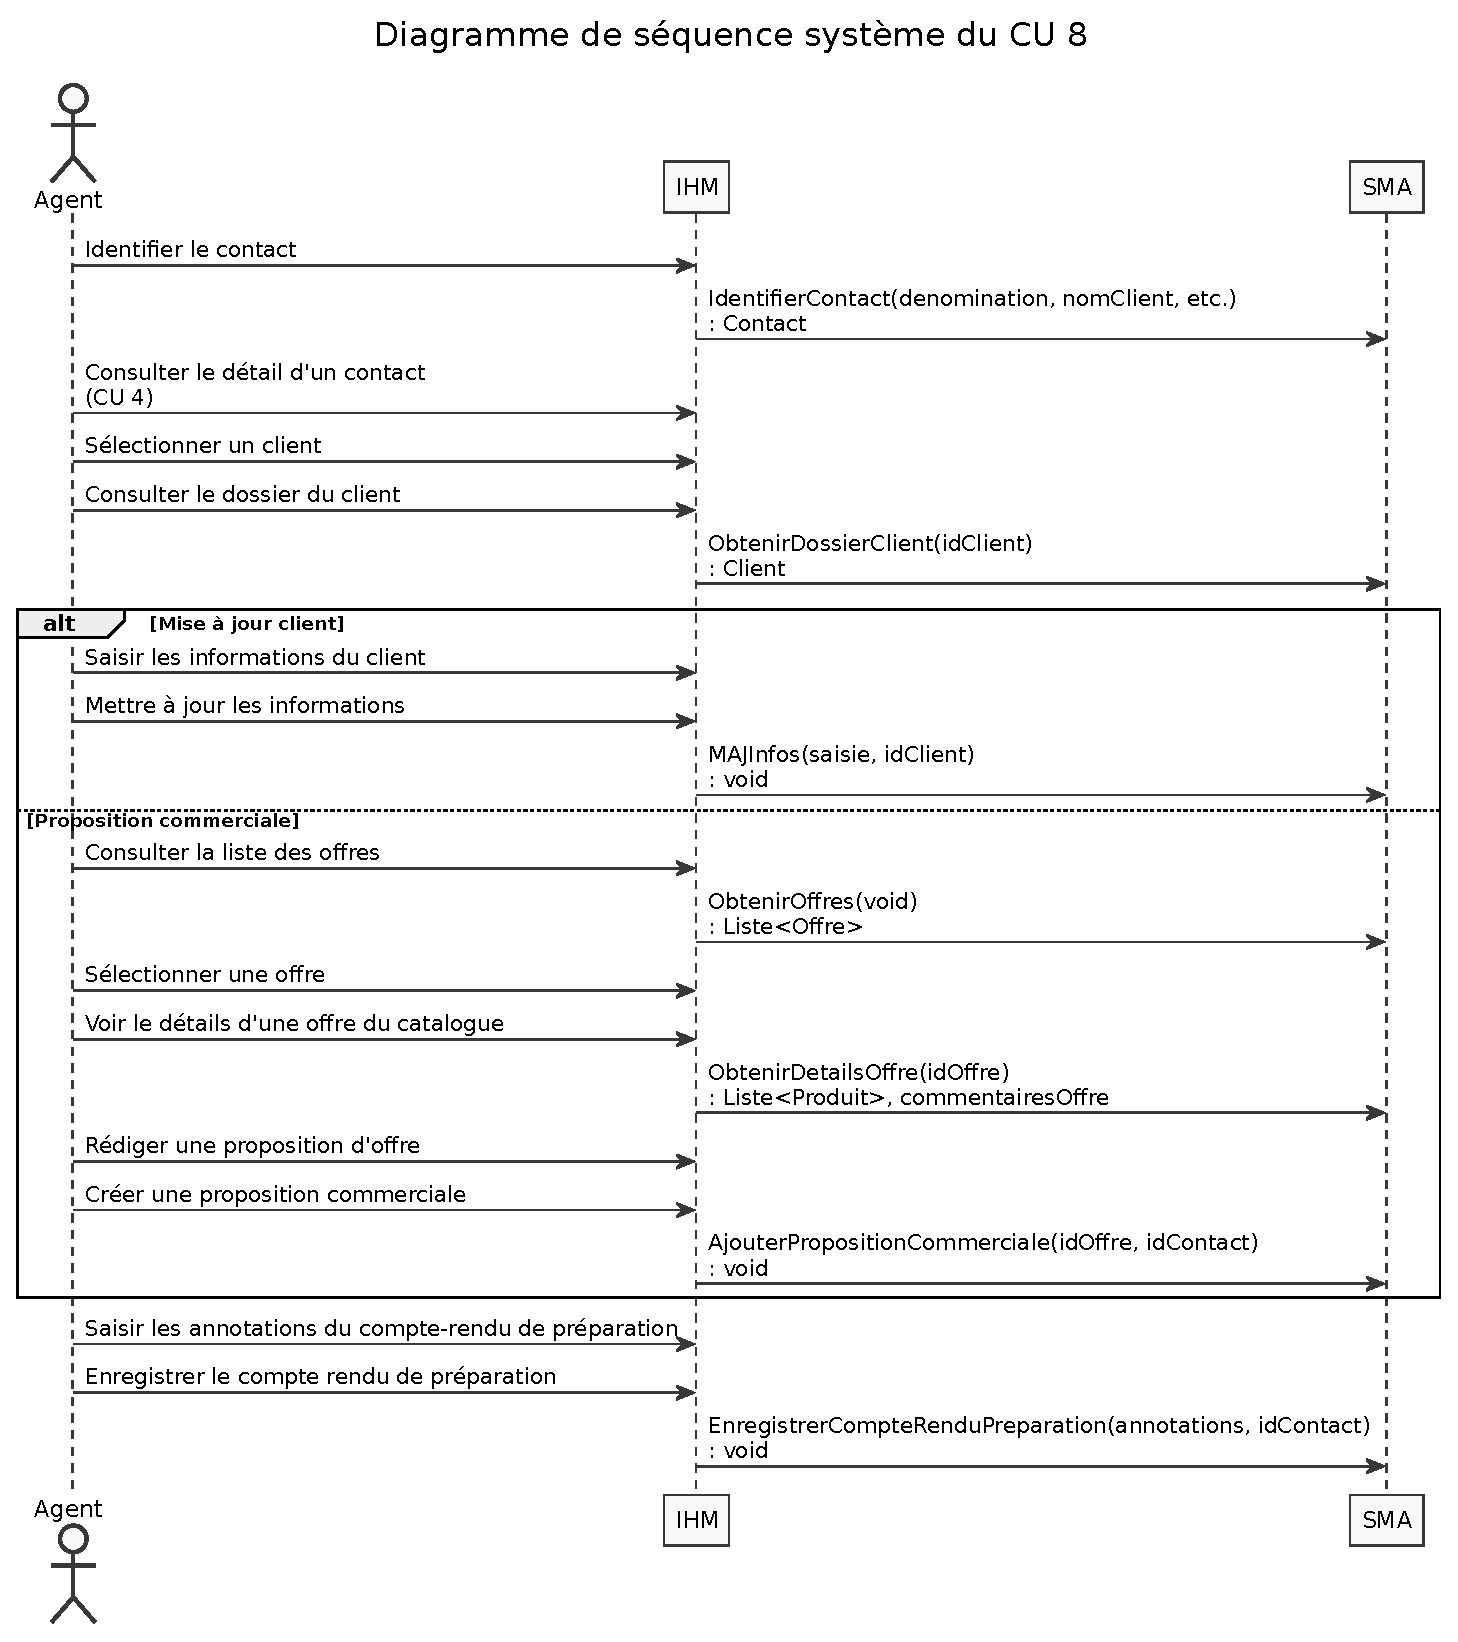
\includegraphics[width=19cm]{figures/eps/DSS_CU8.eps}}
\caption{DSS du CU8}
\end{figure}


\section{CU9 - Conduite de l’entretien par l’agent}

\begin{figure}[H]
\centering
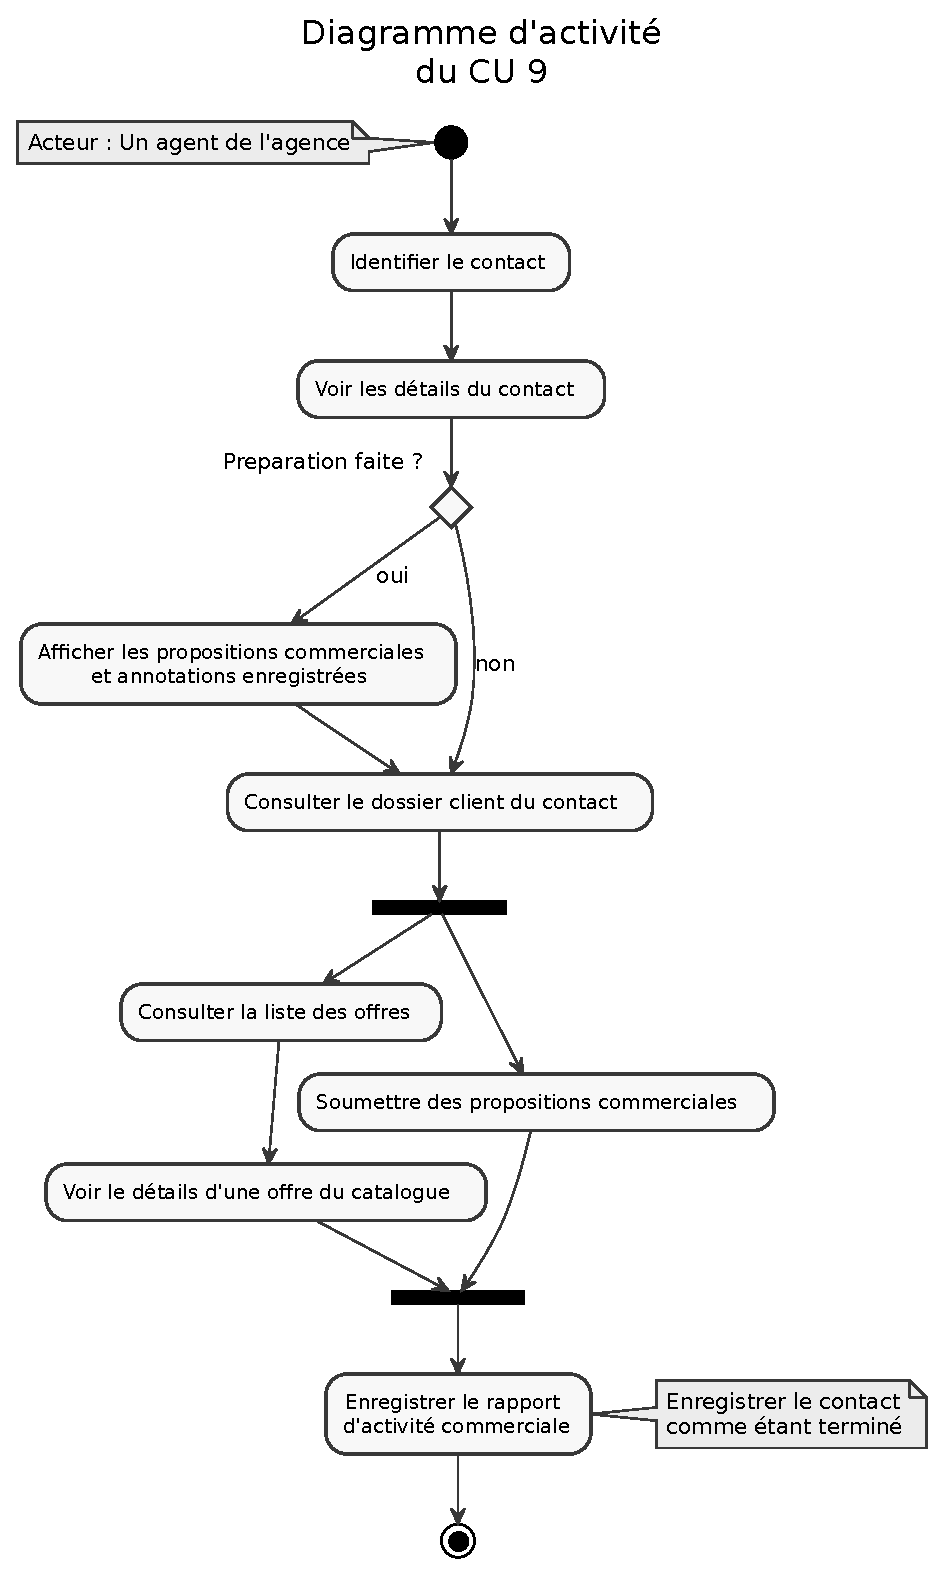
\includegraphics[width=13cm]{figures/eps/DA_CU9.eps}
\caption{DA du CU9}
\end{figure}

\begin{figure}[H]
\noindent\makebox[\textwidth]{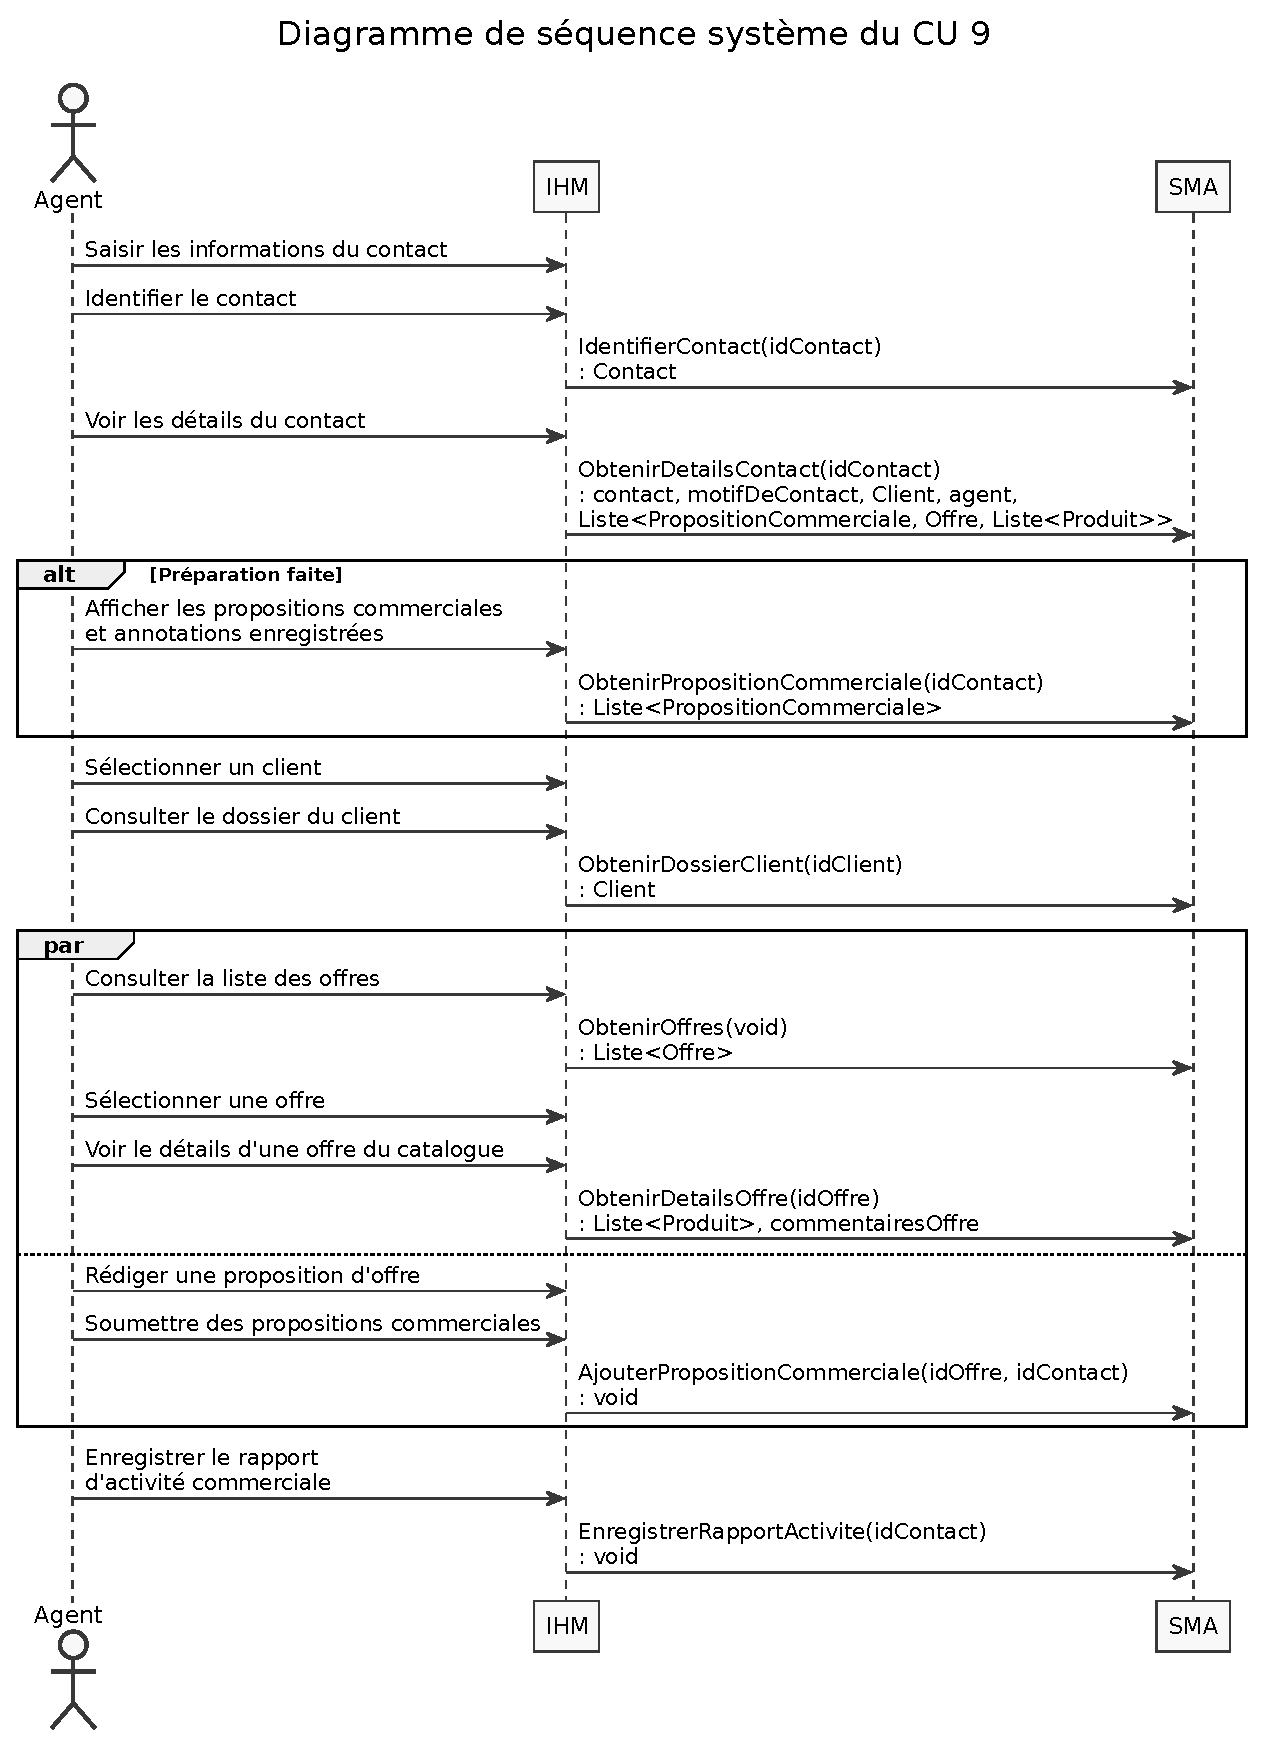
\includegraphics[width=19cm]{figures/eps/DSS_CU9.eps}}
\caption{DSS du CU9}
\end{figure}


\section{CU10 - Consultation du dossier client}
\begin{figure}[H]
\centering
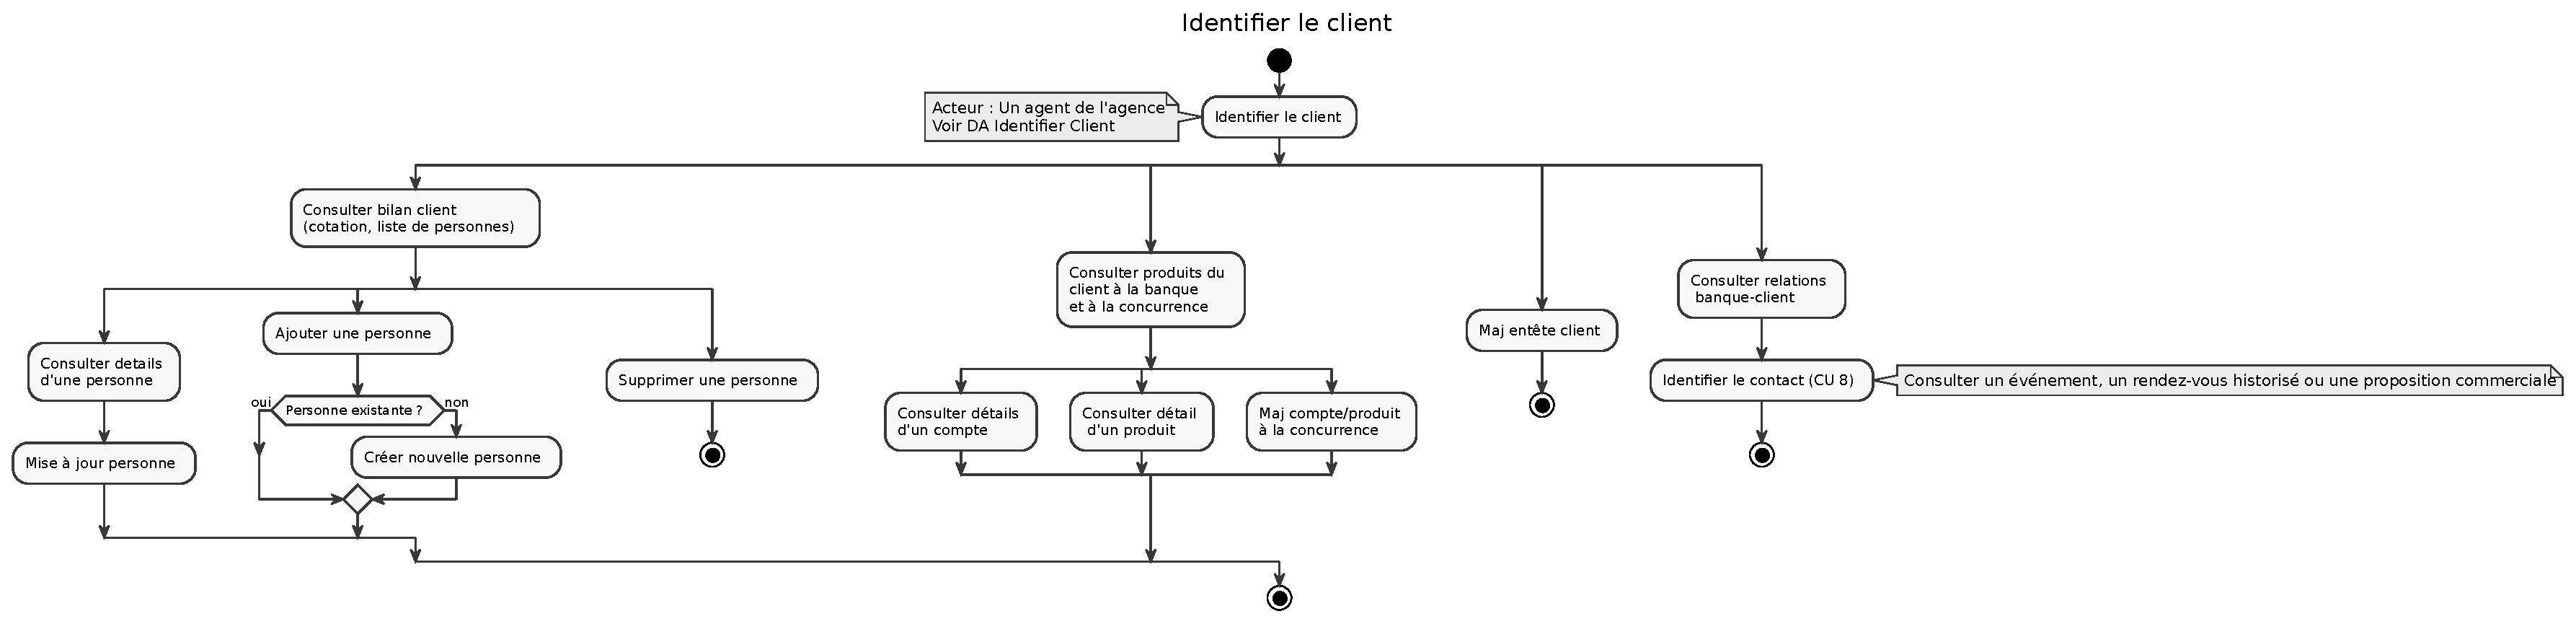
\includegraphics[width=24cm, angle=90]{figures/eps/DA_CU10.eps}
\caption{DA du CU10}
\end{figure}


\begin{figure}[H]
\noindent\makebox[\textwidth]{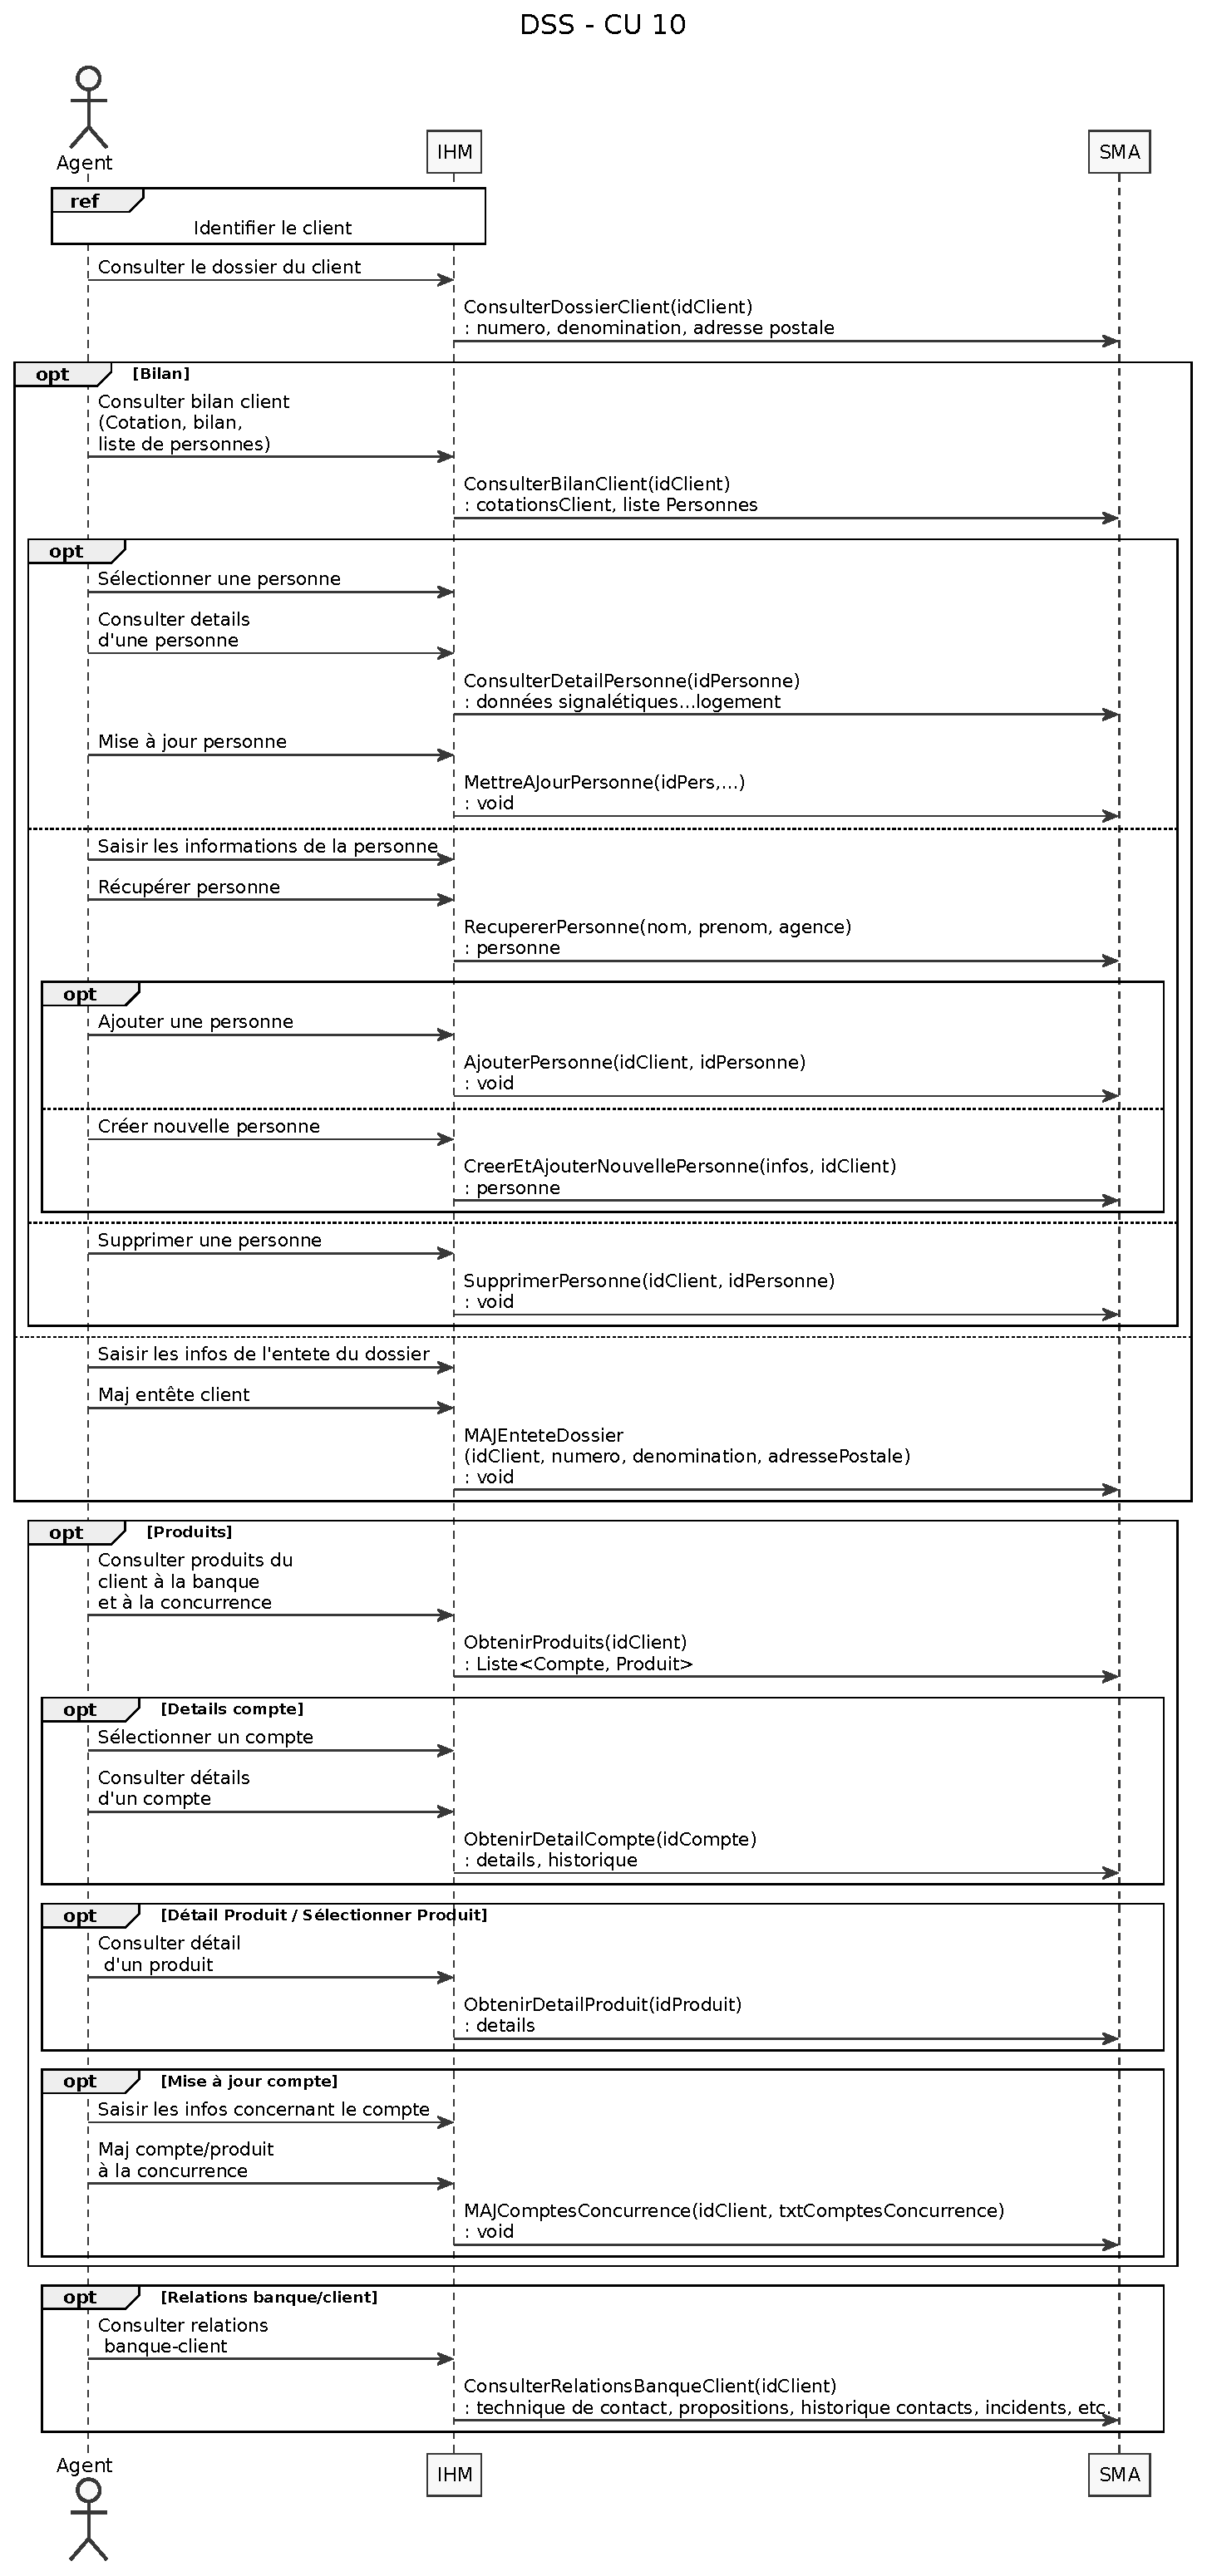
\includegraphics[width=10cm]{figures/eps/DSS_CU10.eps}}
\caption{DSS du CU10}
\end{figure}

\part{IHM}
\setcounter{section}{0}

\section{Enchainement des fenêtres - EDF}

\section{Présentation des différentes vues}

\part{Conception applicative détaillée}

\section{Identification des services et la dynamique de l’architecture}


\subsection{CU1 - Génération de contacts}
\begin{figure}[H]
\noindent\makebox[\textwidth]{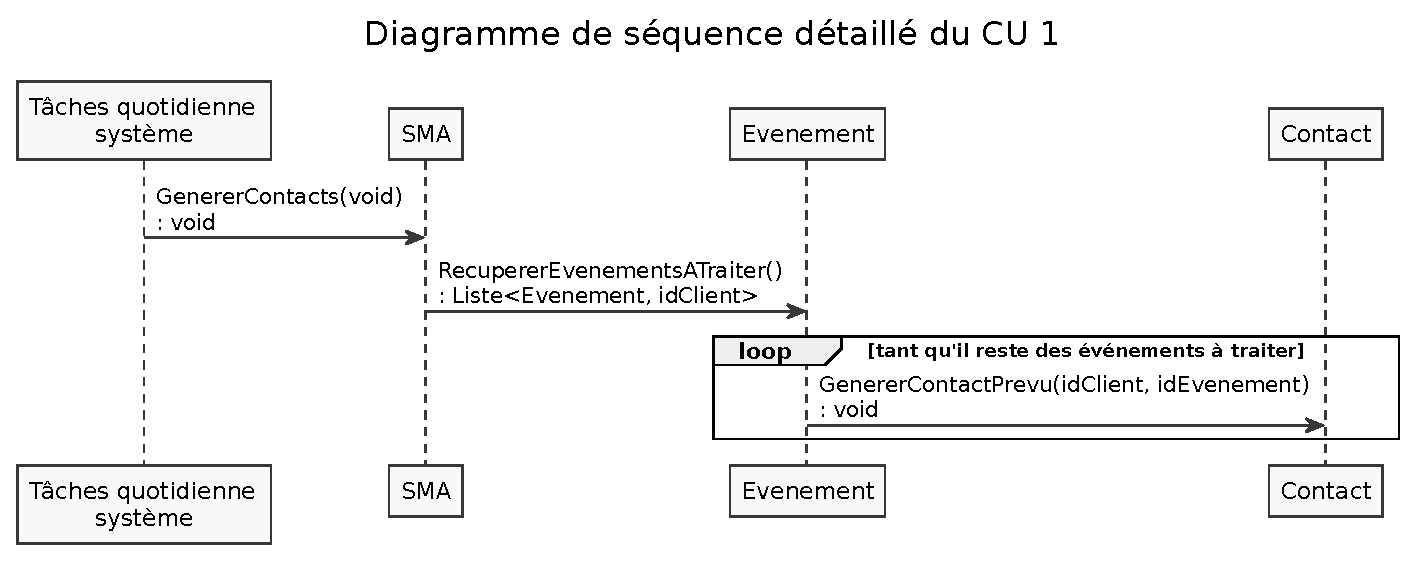
\includegraphics[width=19cm]{figures/eps/DSD_CU1.eps}}
\caption{DSD du CU1}
\end{figure}

\subsection{CU2 - Répartition des contacts commerciaux}
\begin{figure}[H]
\noindent\makebox[\textwidth]{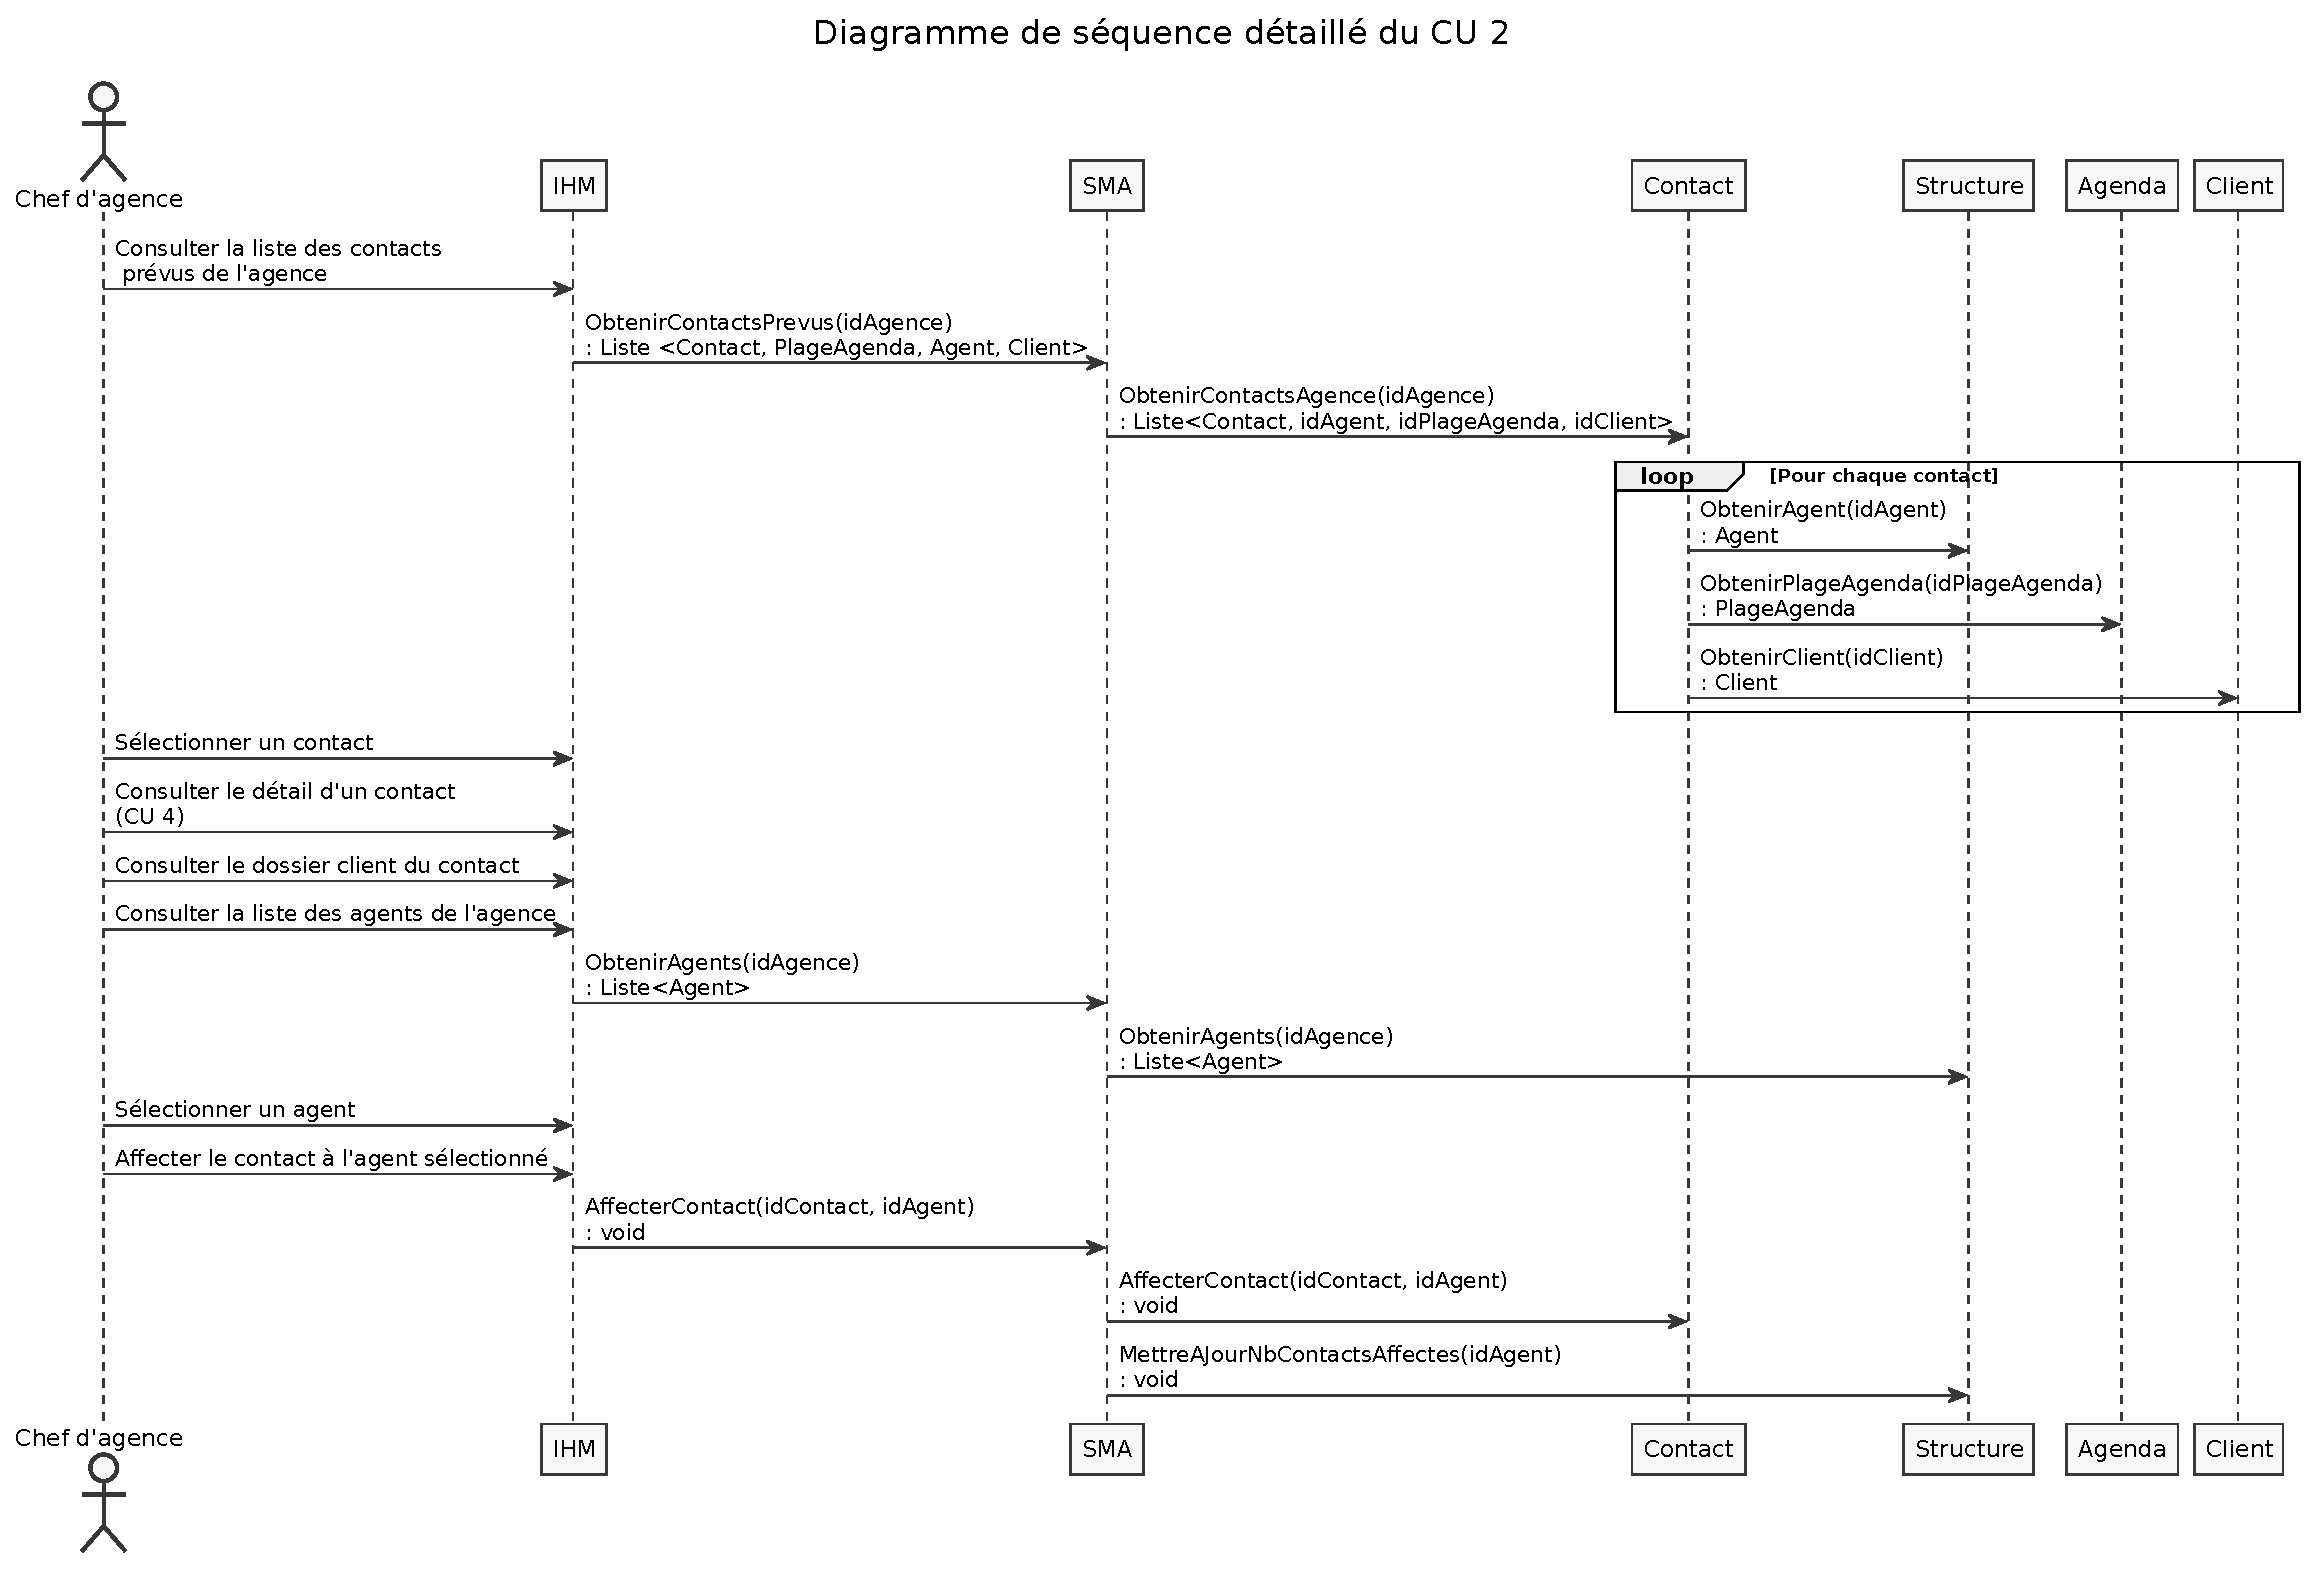
\includegraphics[width=23cm, angle=90]{figures/eps/DSD_CU2.eps}}
\caption{DSD du CU2}
\end{figure}


\subsection{CU3 - Suivi de l’action commercial}
\begin{figure}[H]
\noindent\makebox[\textwidth]{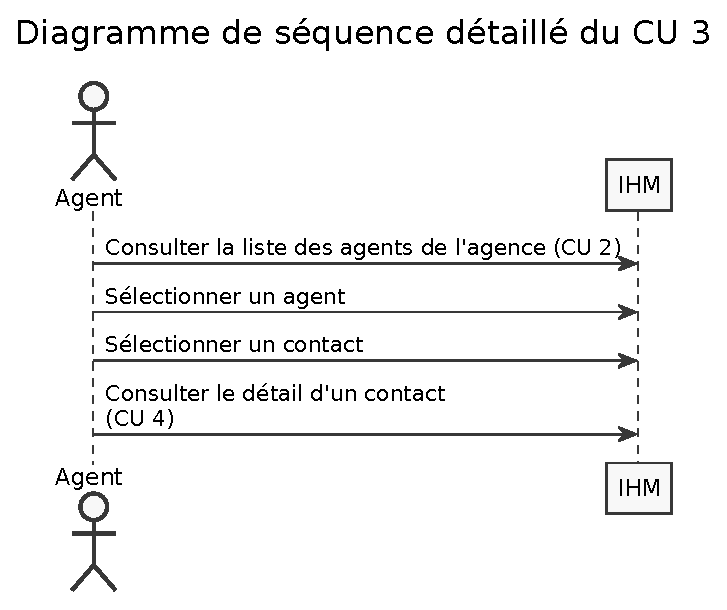
\includegraphics[width=21cm, angle=90]{figures/eps/DSD_CU3.eps}}
\caption{DSD du CU3}
\end{figure}

\subsection{CU4 – Gestion de la liste des contacts clients}
\begin{figure}[H]
\noindent\makebox[\textwidth]{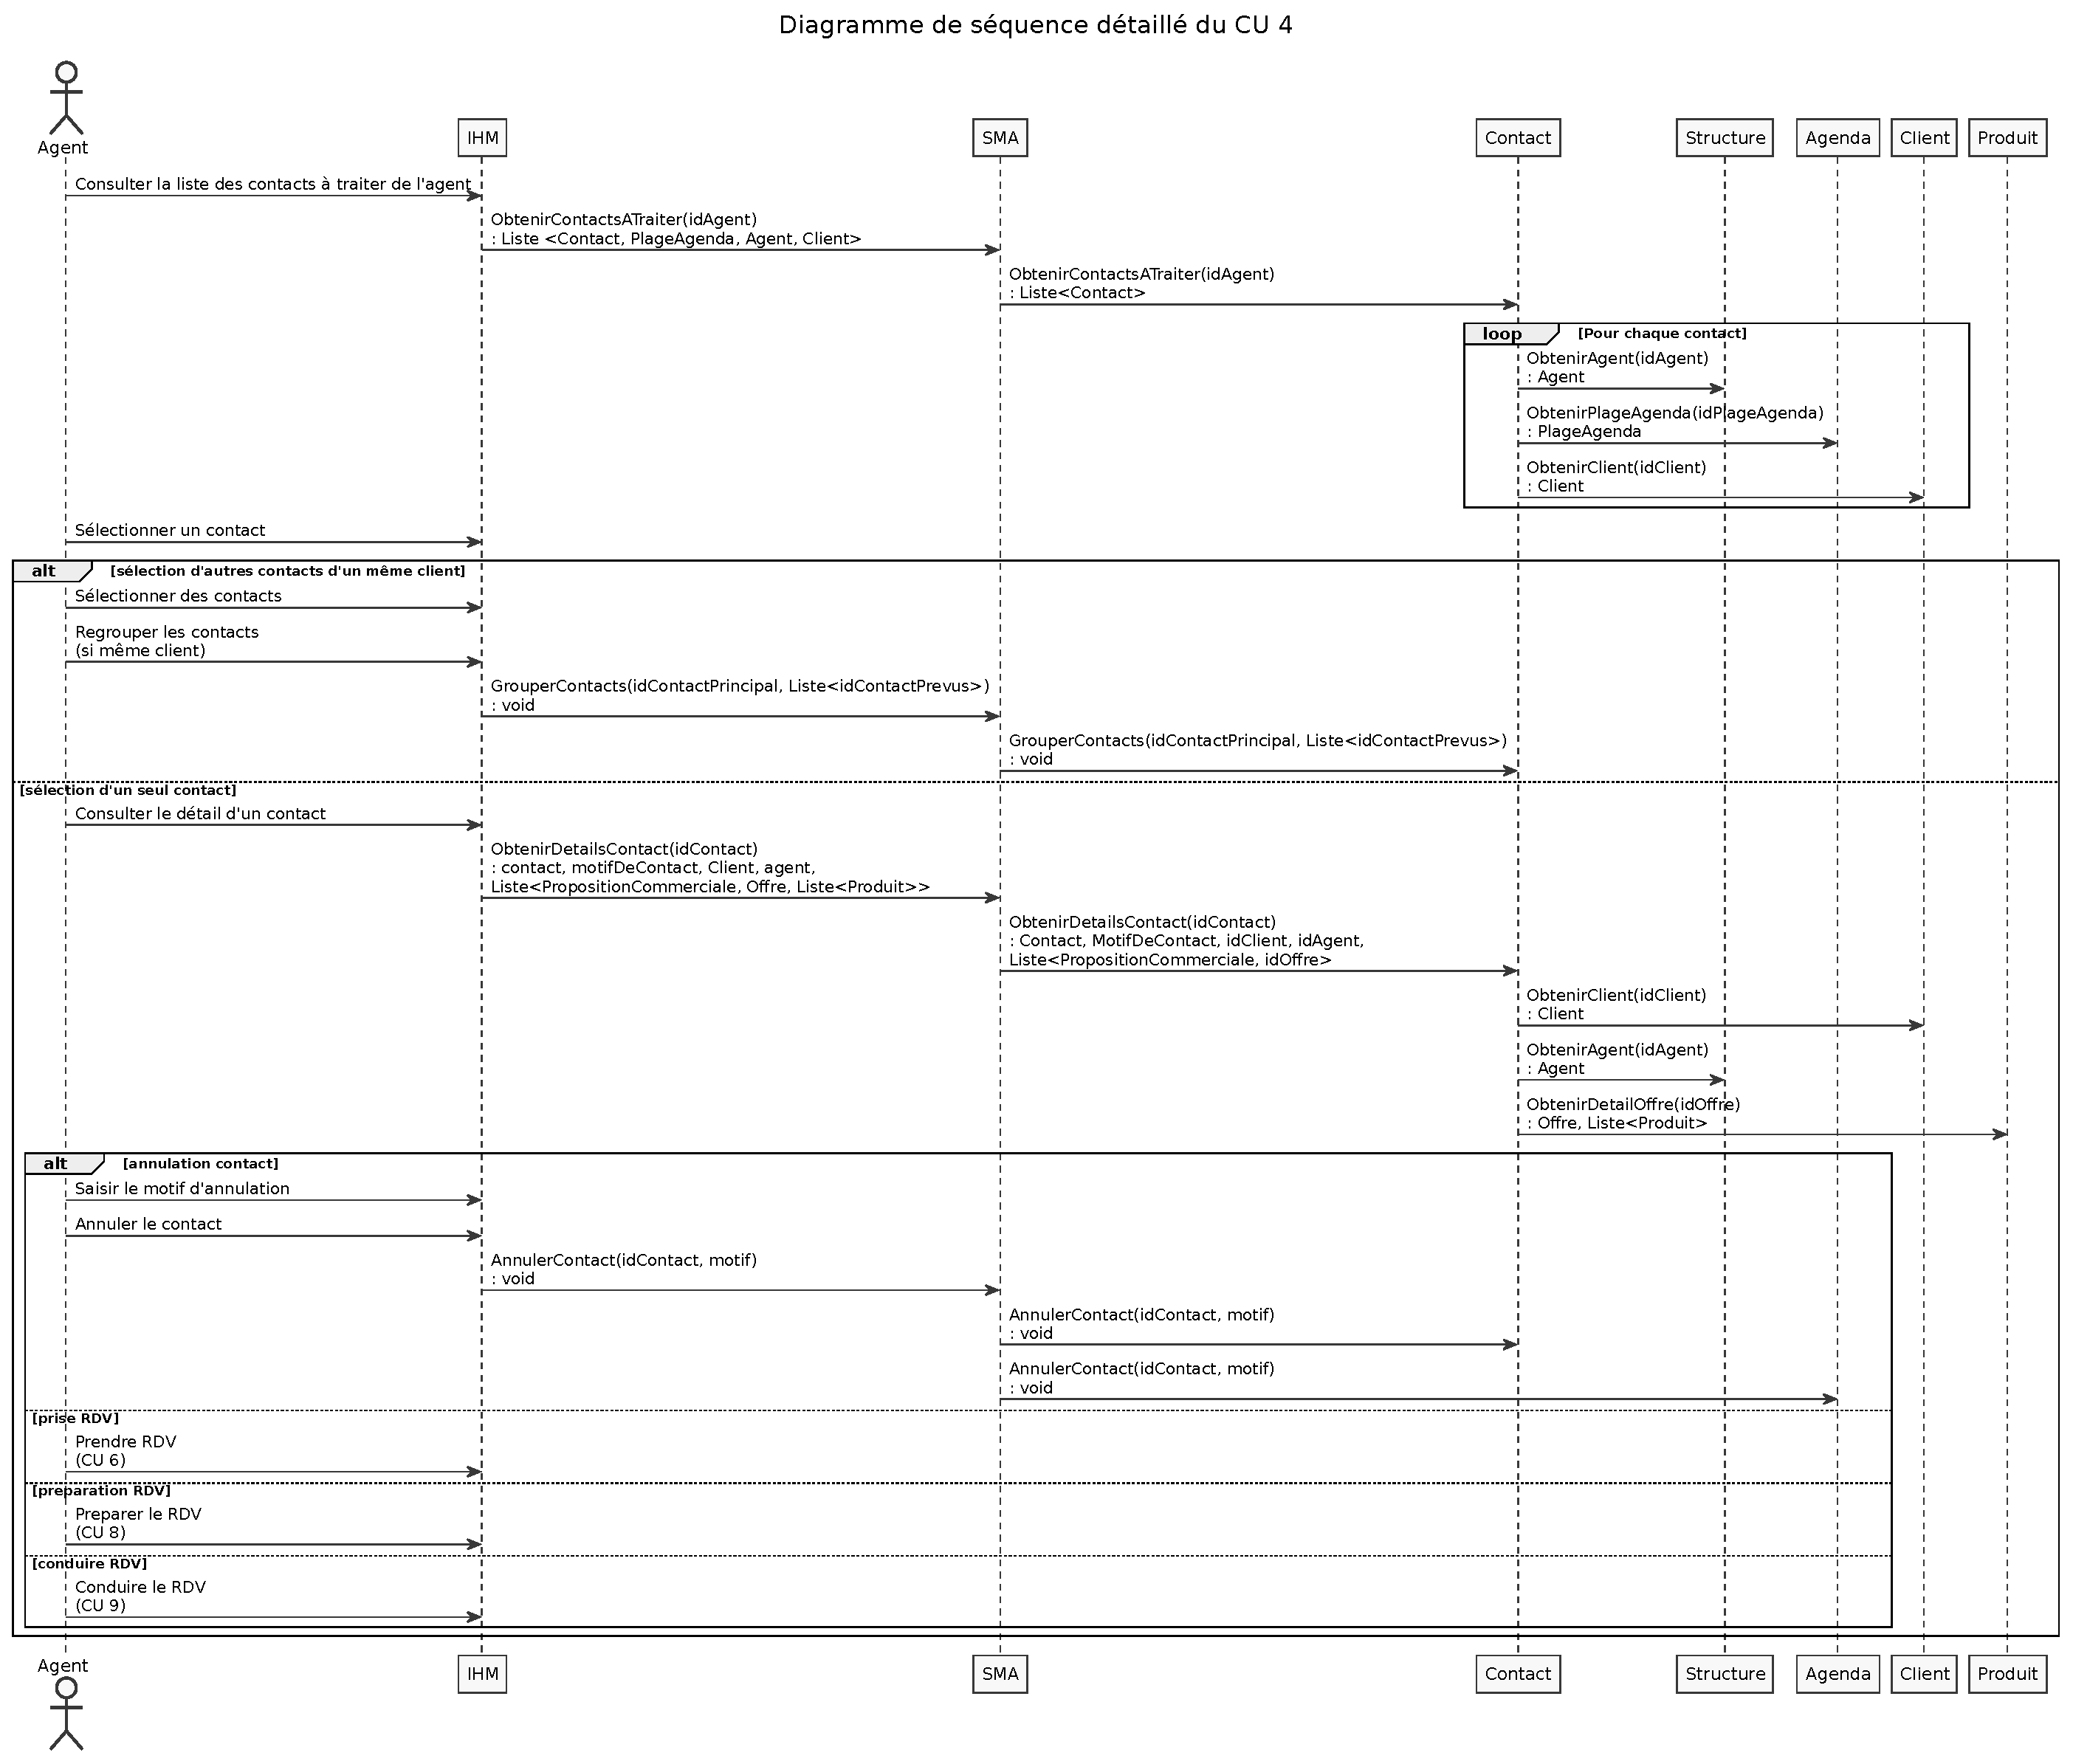
\includegraphics[width=20cm, angle=90]{figures/eps/DSD_CU4.eps}}
\caption{DSD du CU4}
\end{figure}


\subsection{CU5 - Planification de l’activité de l’agence du mois suivant}
\begin{figure}[H]
\noindent\makebox[\textwidth]{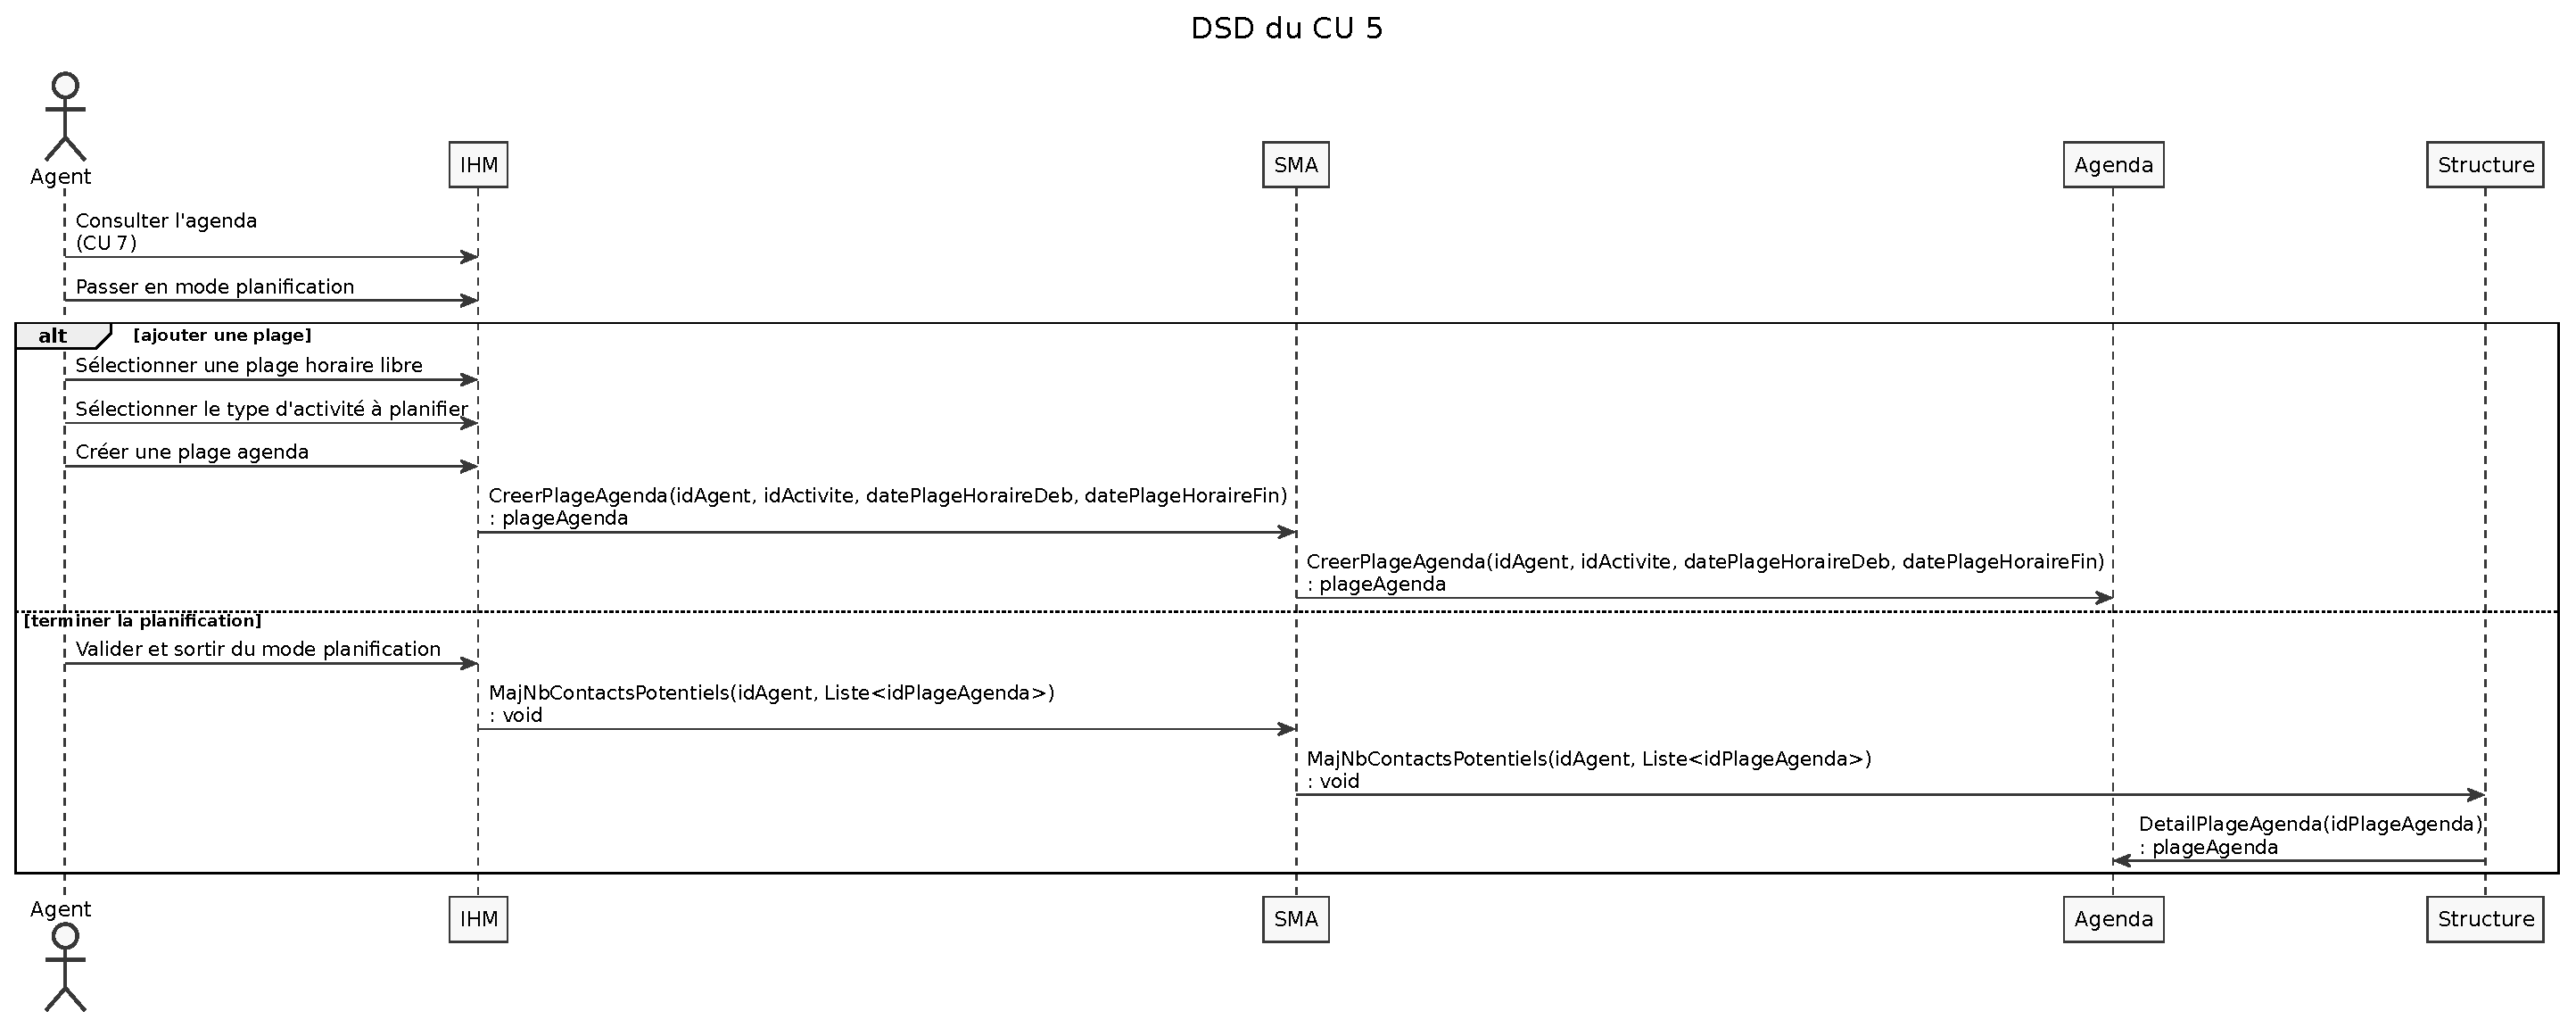
\includegraphics[width=24cm, angle=90]{figures/eps/DSD_CU5.eps}}
\caption{DSD du CU5}
\end{figure}


\subsection{CU6 - Planification des contacts commerciaux}

\subsubsection{contacts commerciaux}
\begin{figure}[H]
\noindent\makebox[\textwidth]{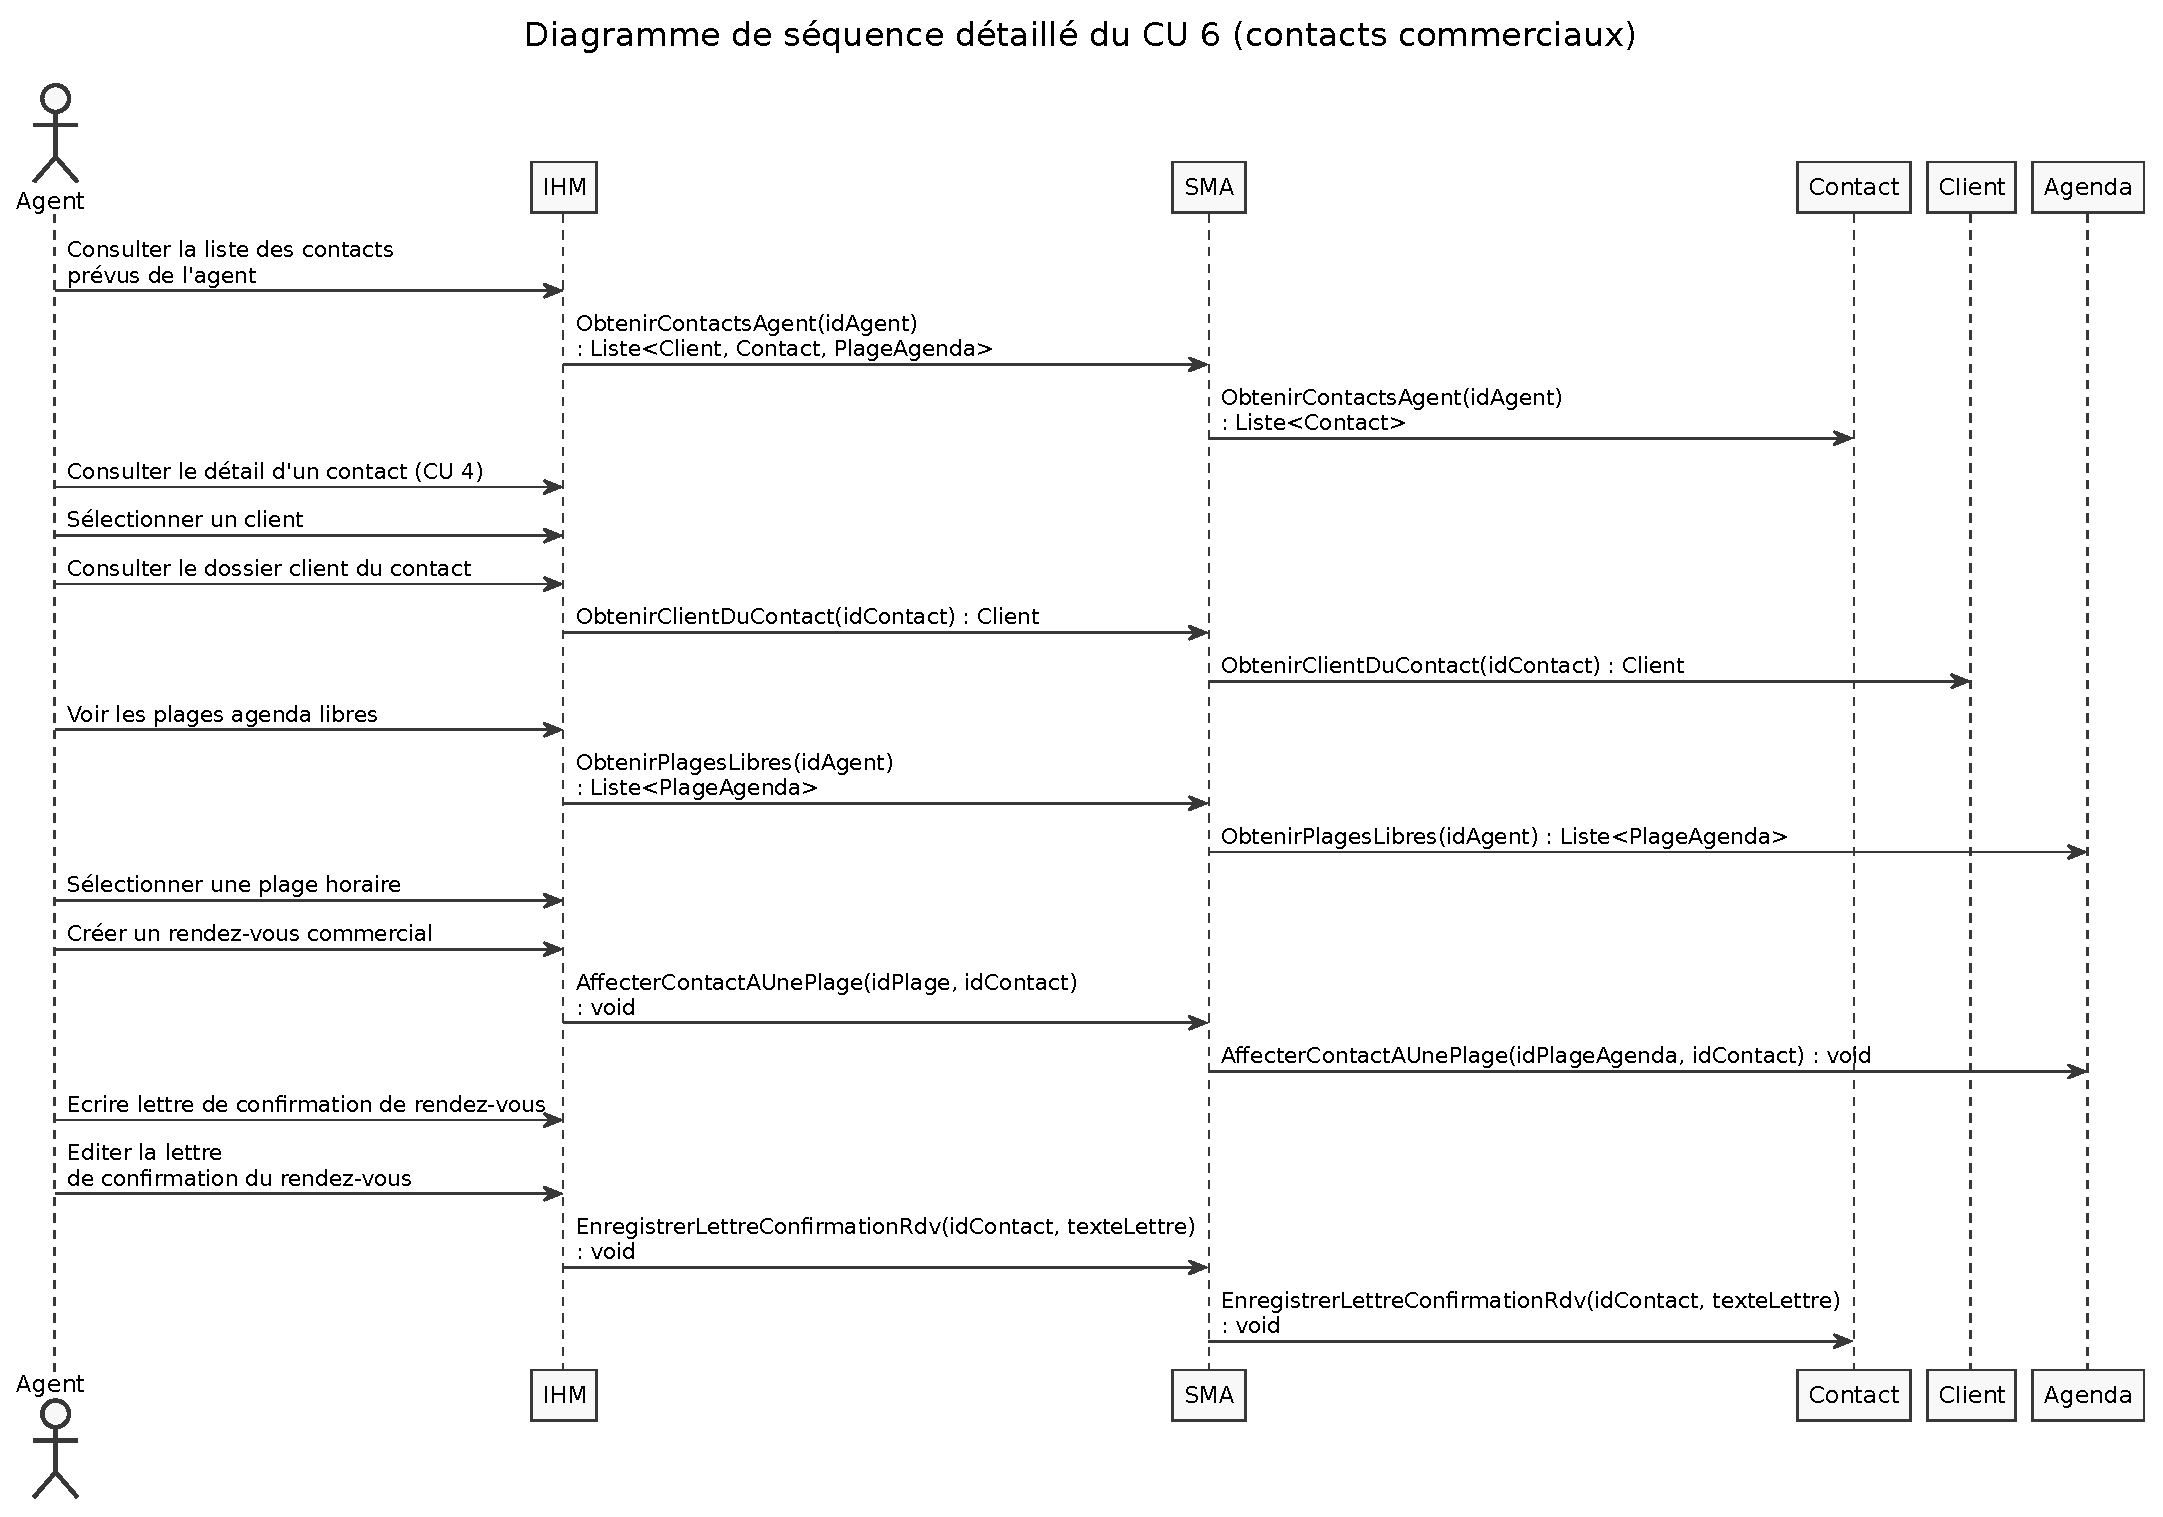
\includegraphics[width=23cm, angle=90]{figures/eps/DSD_CU6_partieAgent.eps}}
\caption{DSD "contacts commerciaux" du CU6}
\end{figure}

\subsubsection{contacts spontanés}
\begin{figure}[H]
\noindent\makebox[\textwidth]{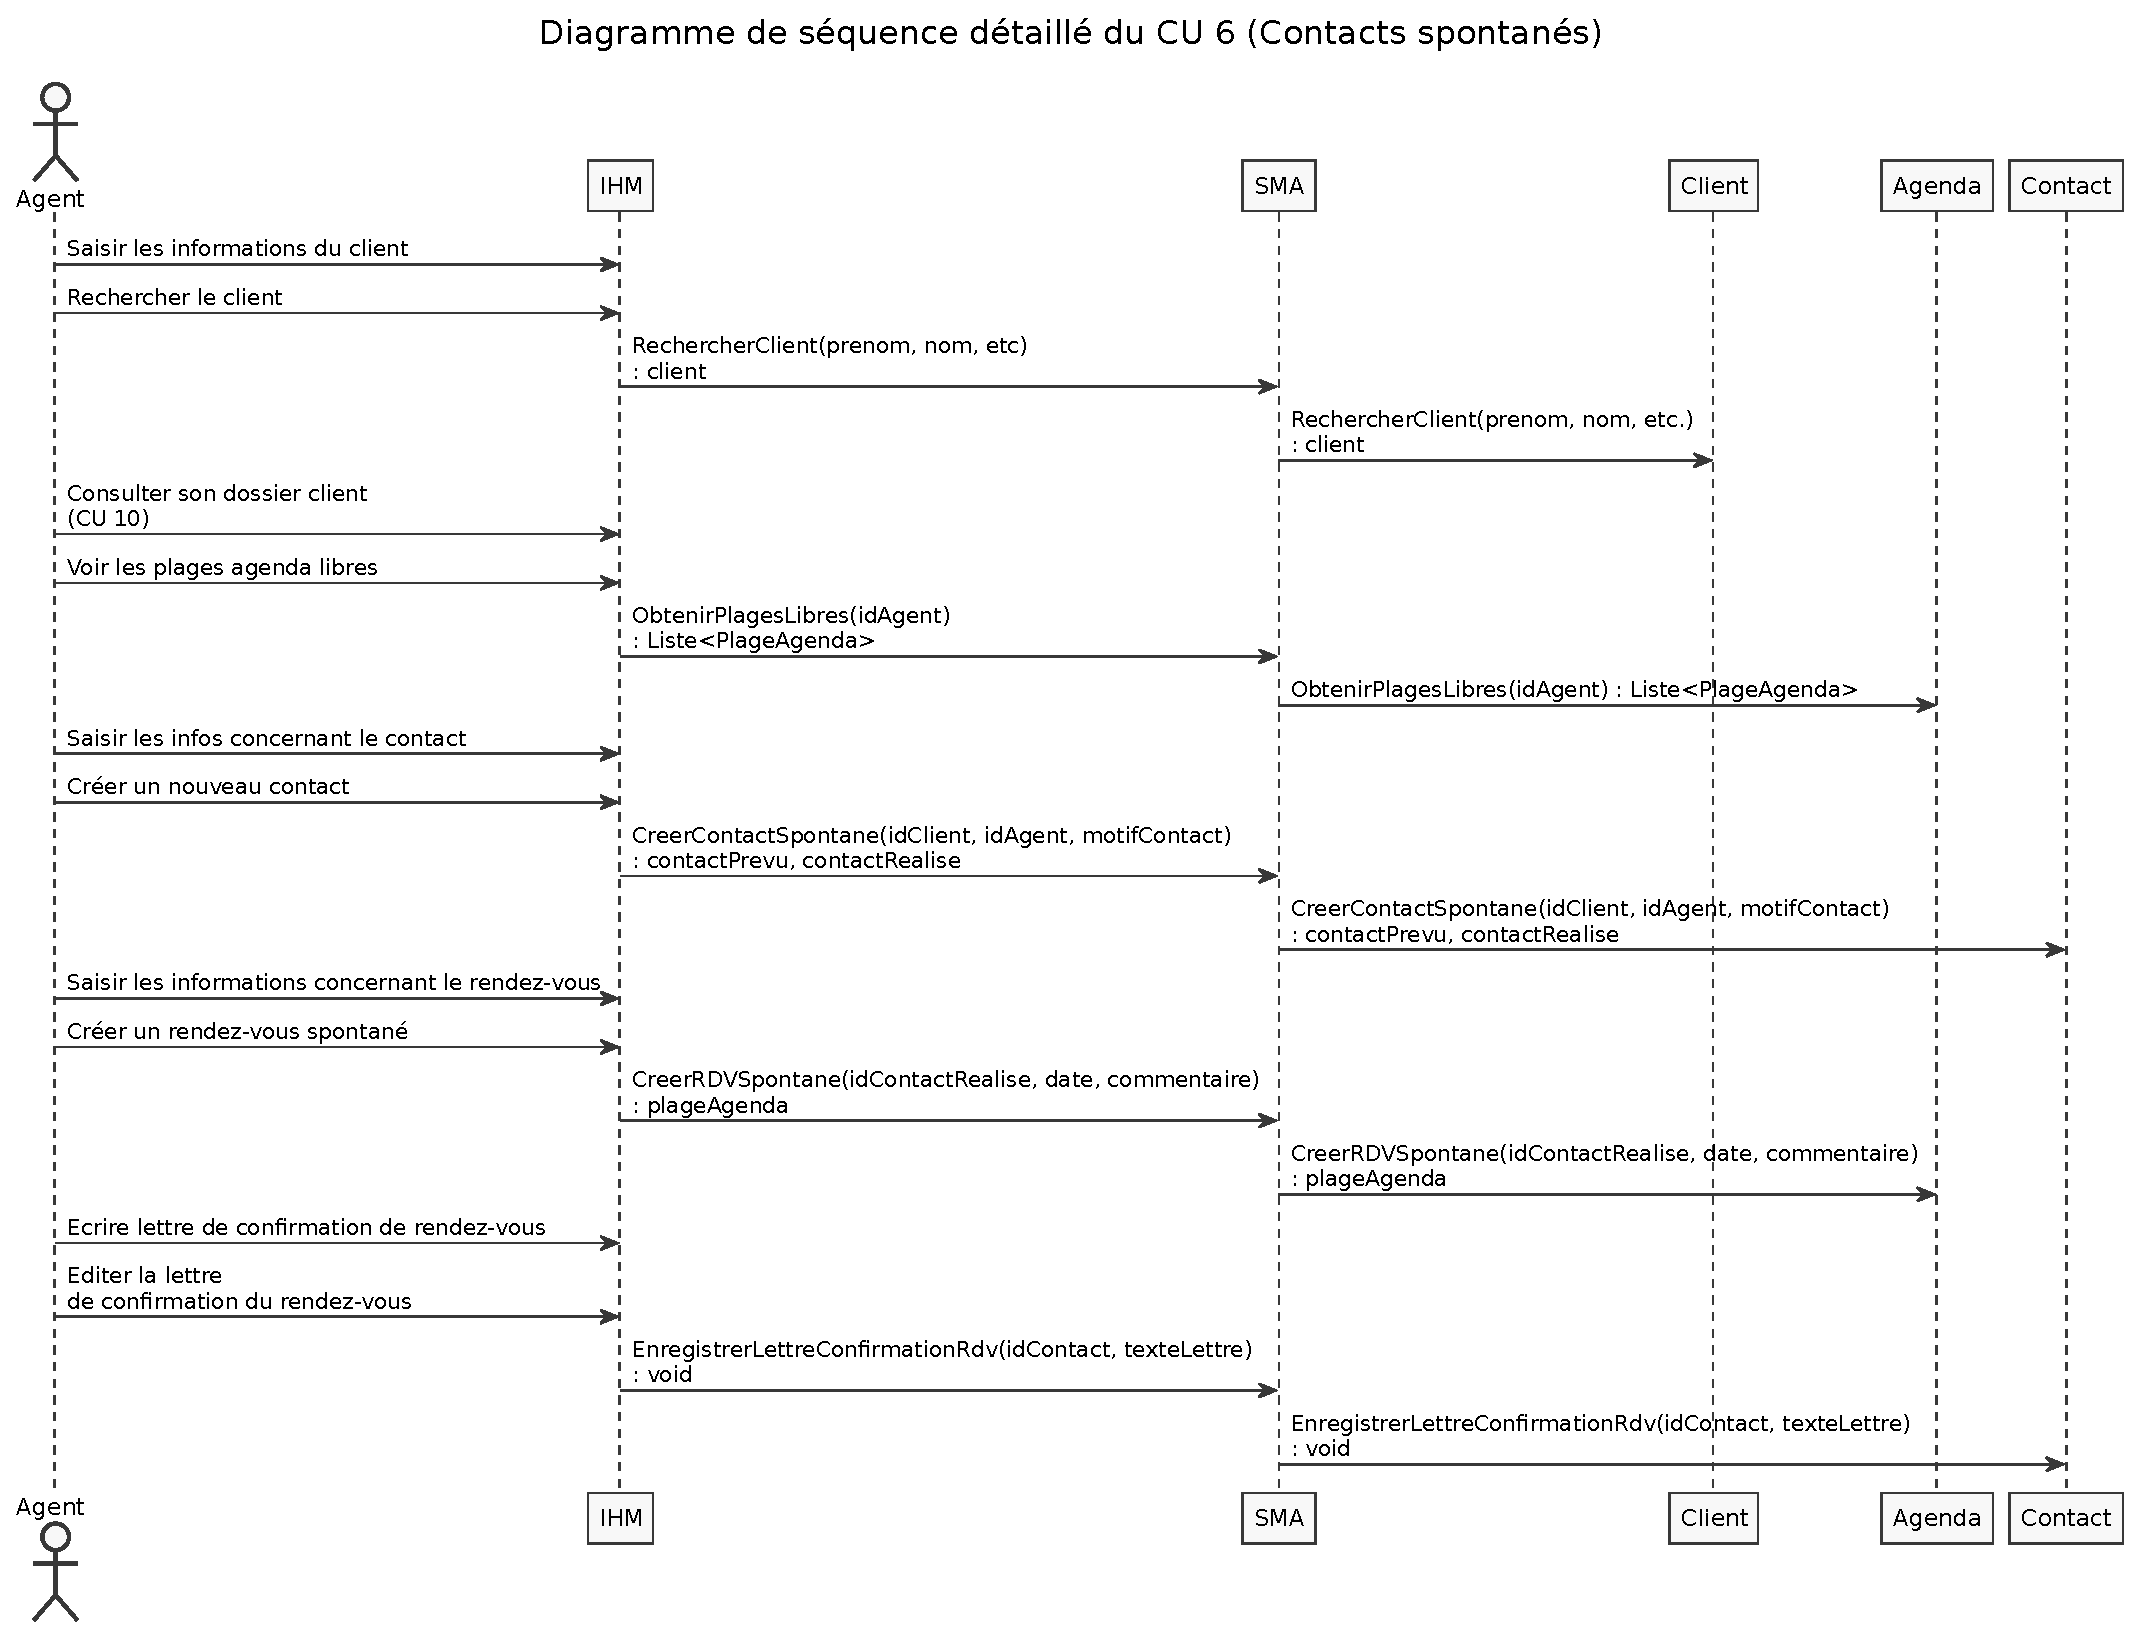
\includegraphics[width=23cm, angle=90]{figures/eps/DSD_CU6_partieClient.eps}}
\caption{DSD "contacts spontanés" du CU6}
\end{figure}


\subsection{CU7 - Consultation des agendas}
\begin{figure}[H]
\noindent\makebox[\textwidth]{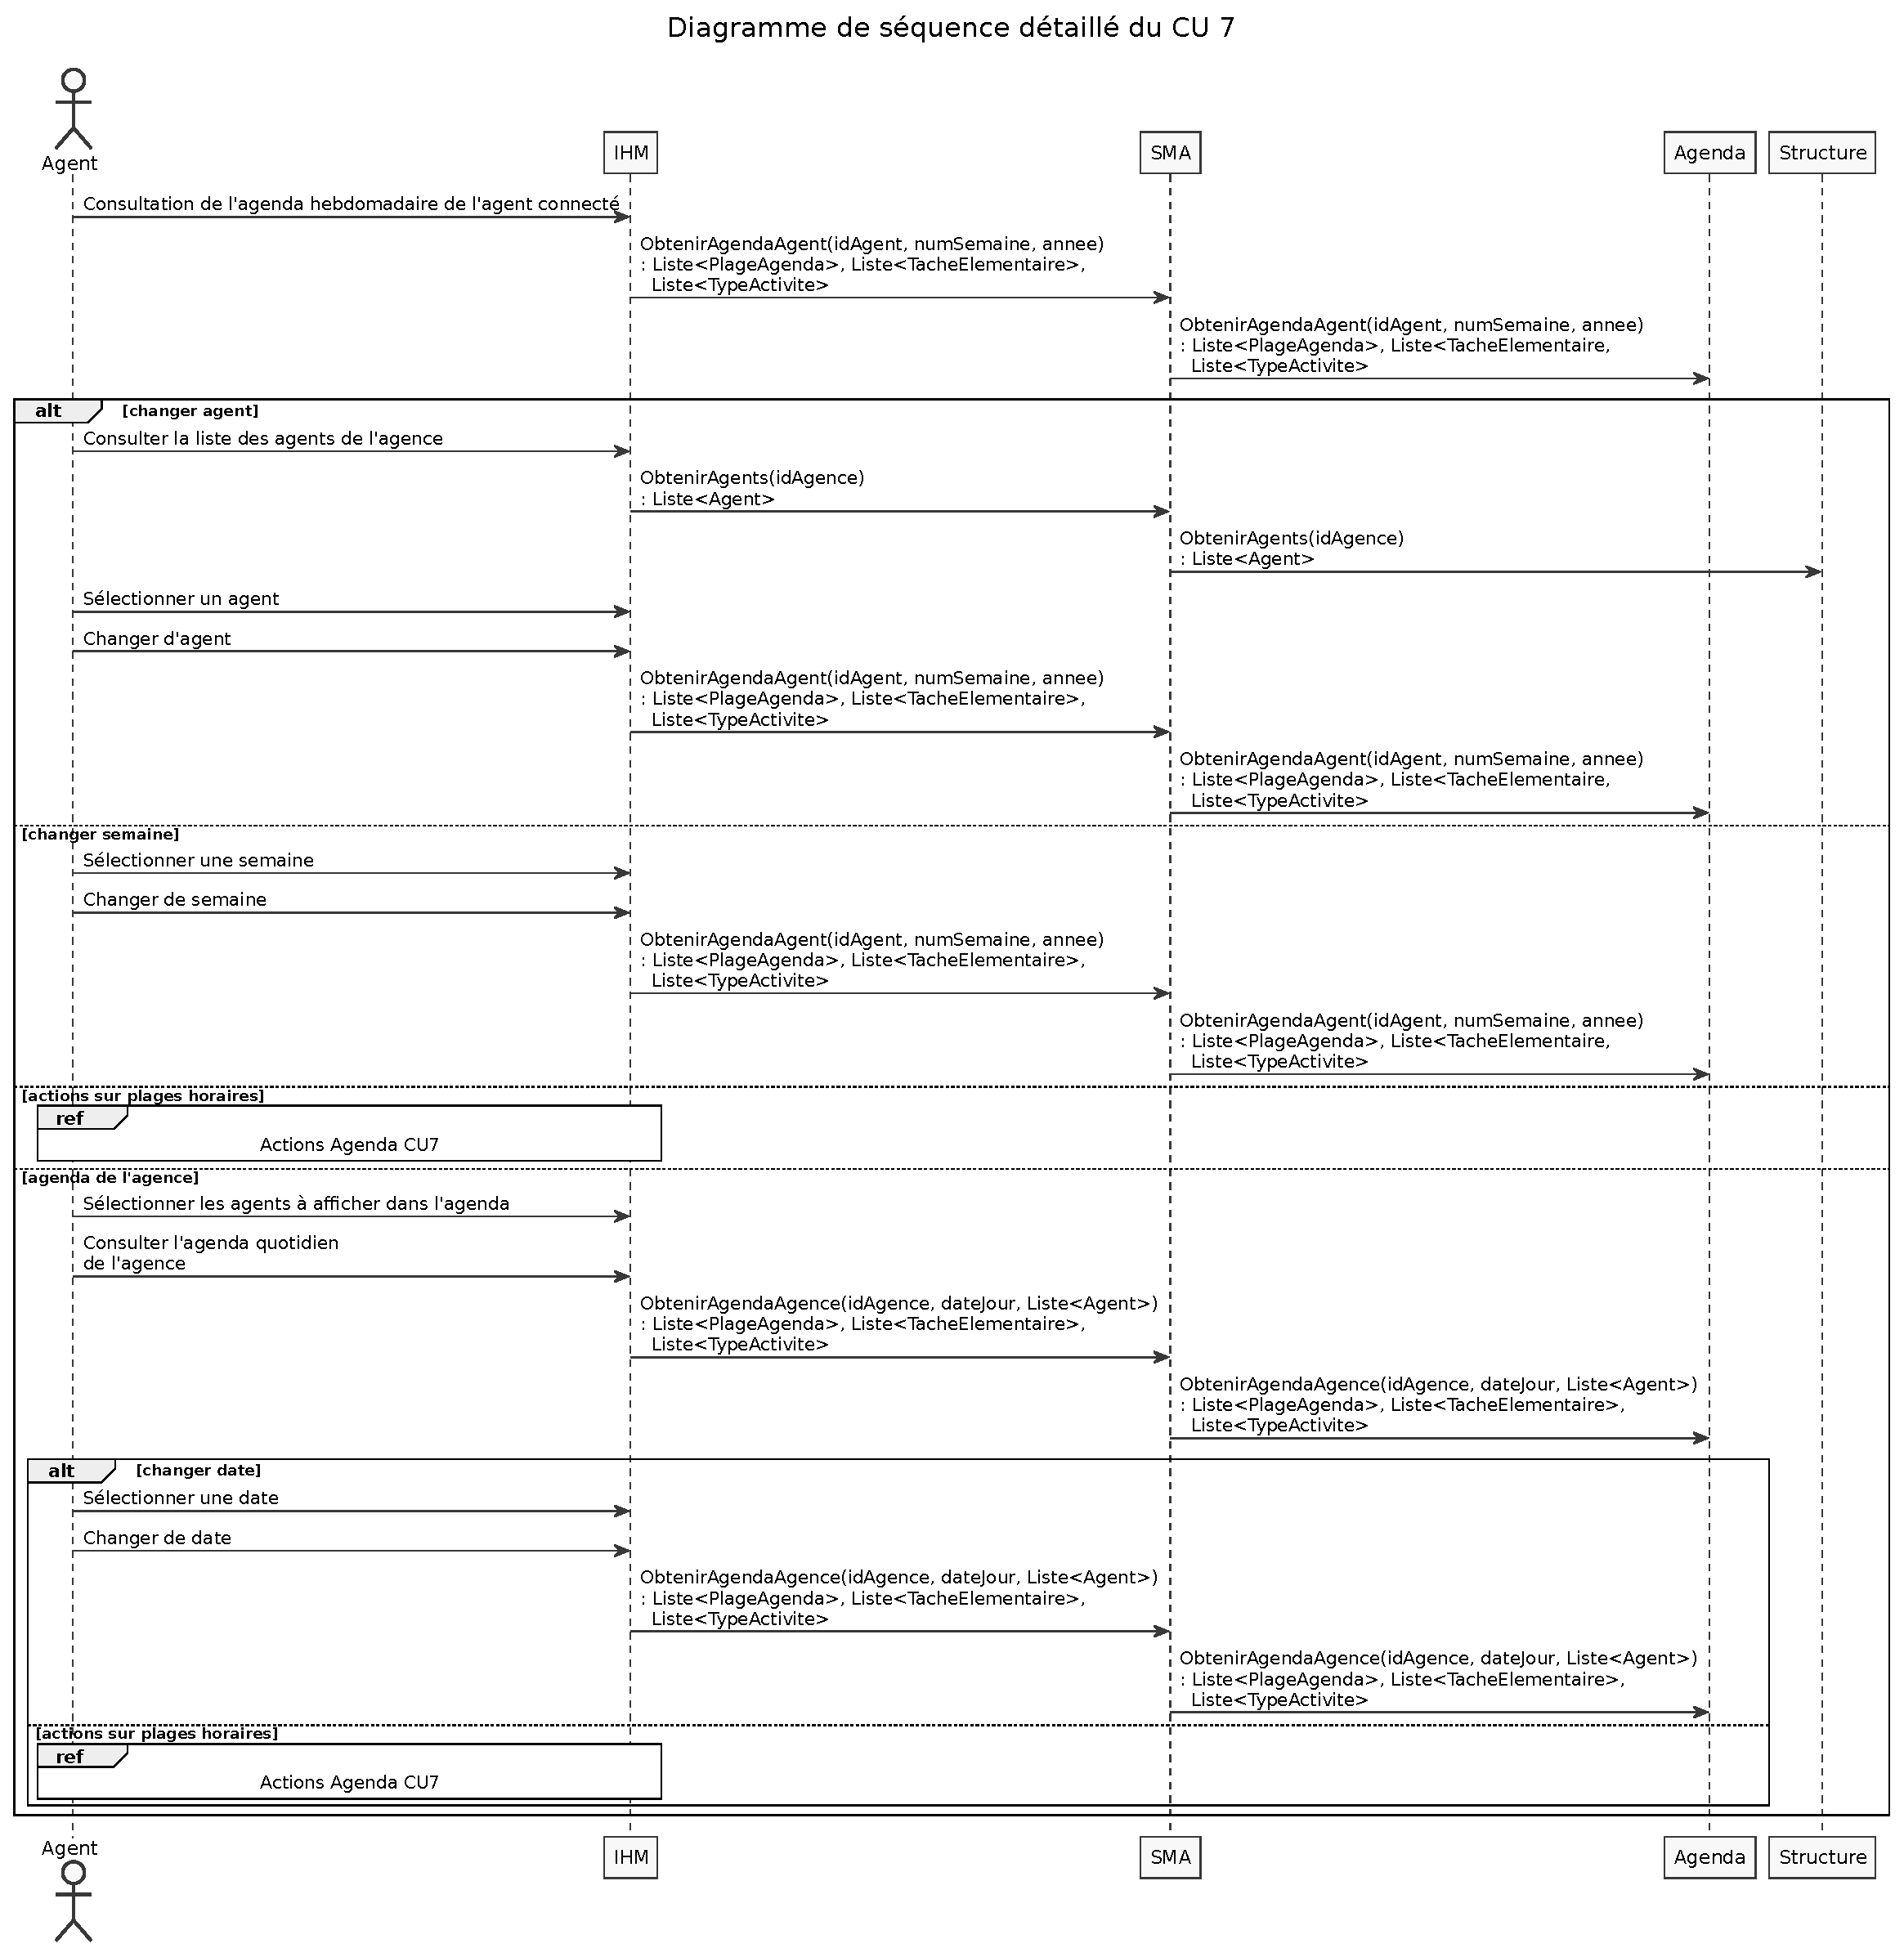
\includegraphics[width=19cm]{figures/eps/DSD_CU7.eps}}
\caption{DSD du CU7}
\end{figure}

\begin{figure}[H]
\noindent\makebox[\textwidth]{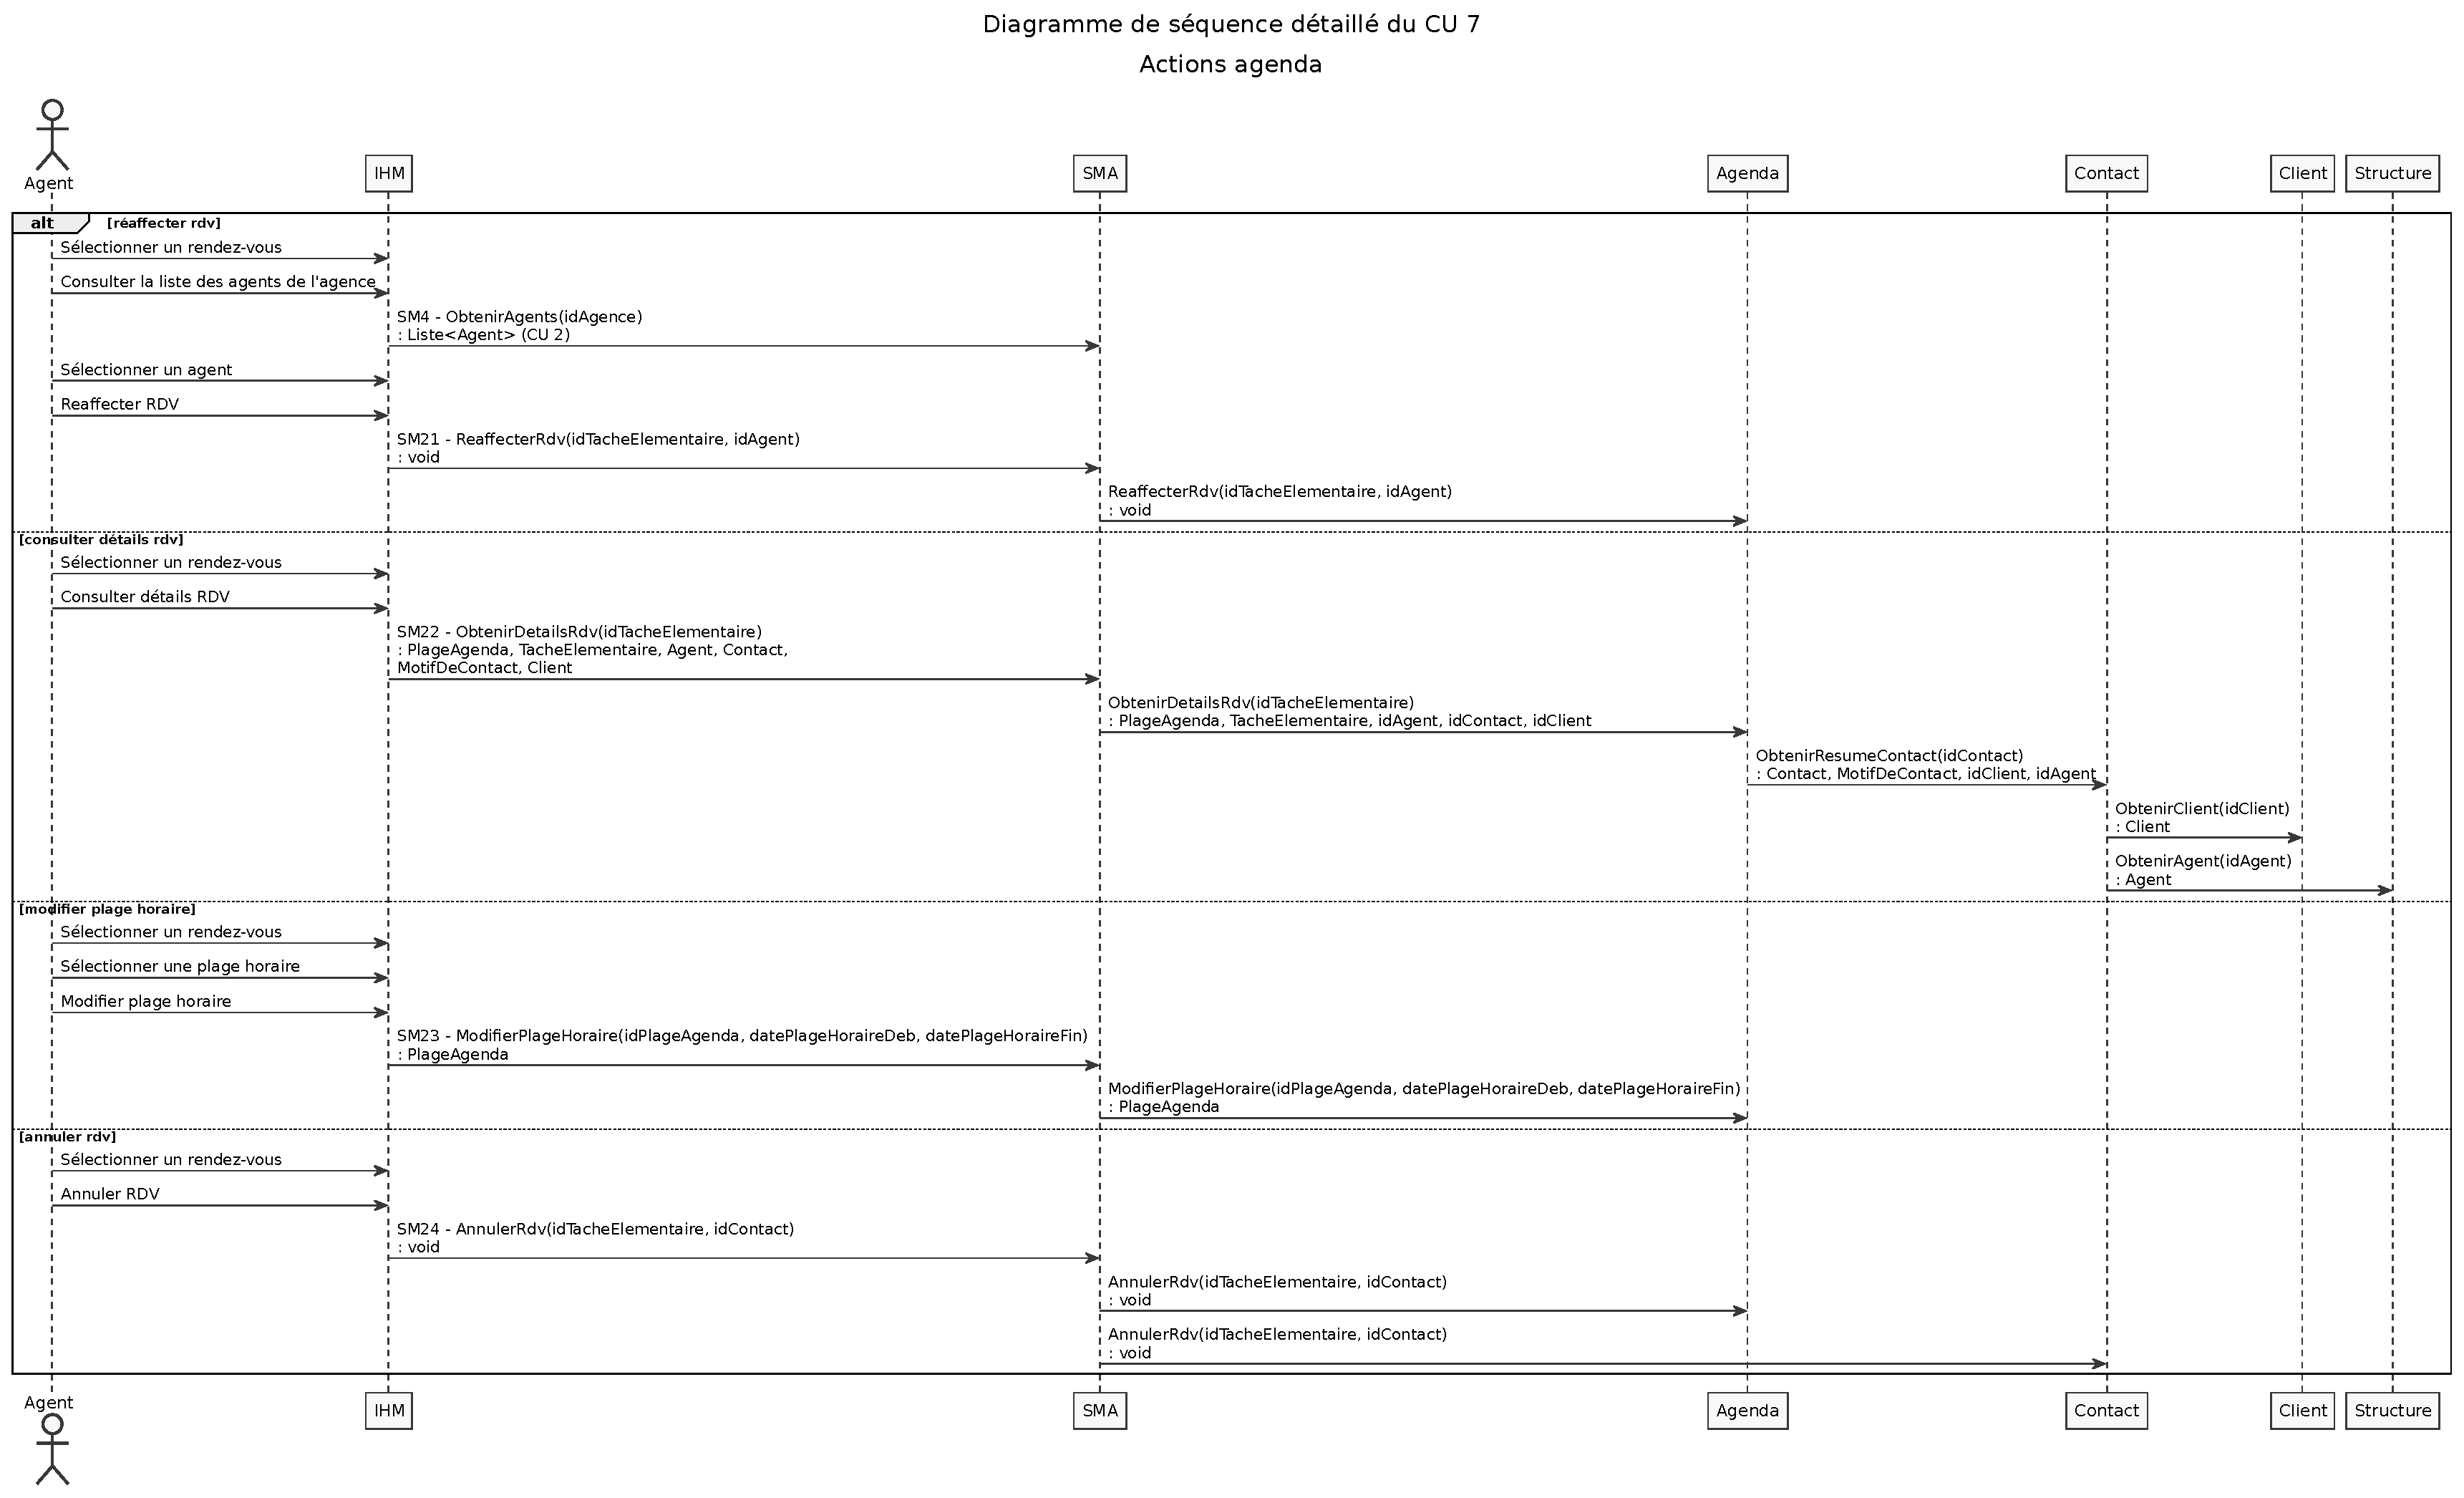
\includegraphics[width=24cm, angle=90]{figures/eps/DSD_CU7_ActionsAgenda}}
\caption{DSD "Actions Agenda" du CU7}
\end{figure}


\subsection{CU8 - Préparation d’entretien par un agent}
\begin{figure}[H]
\noindent\makebox[\textwidth]{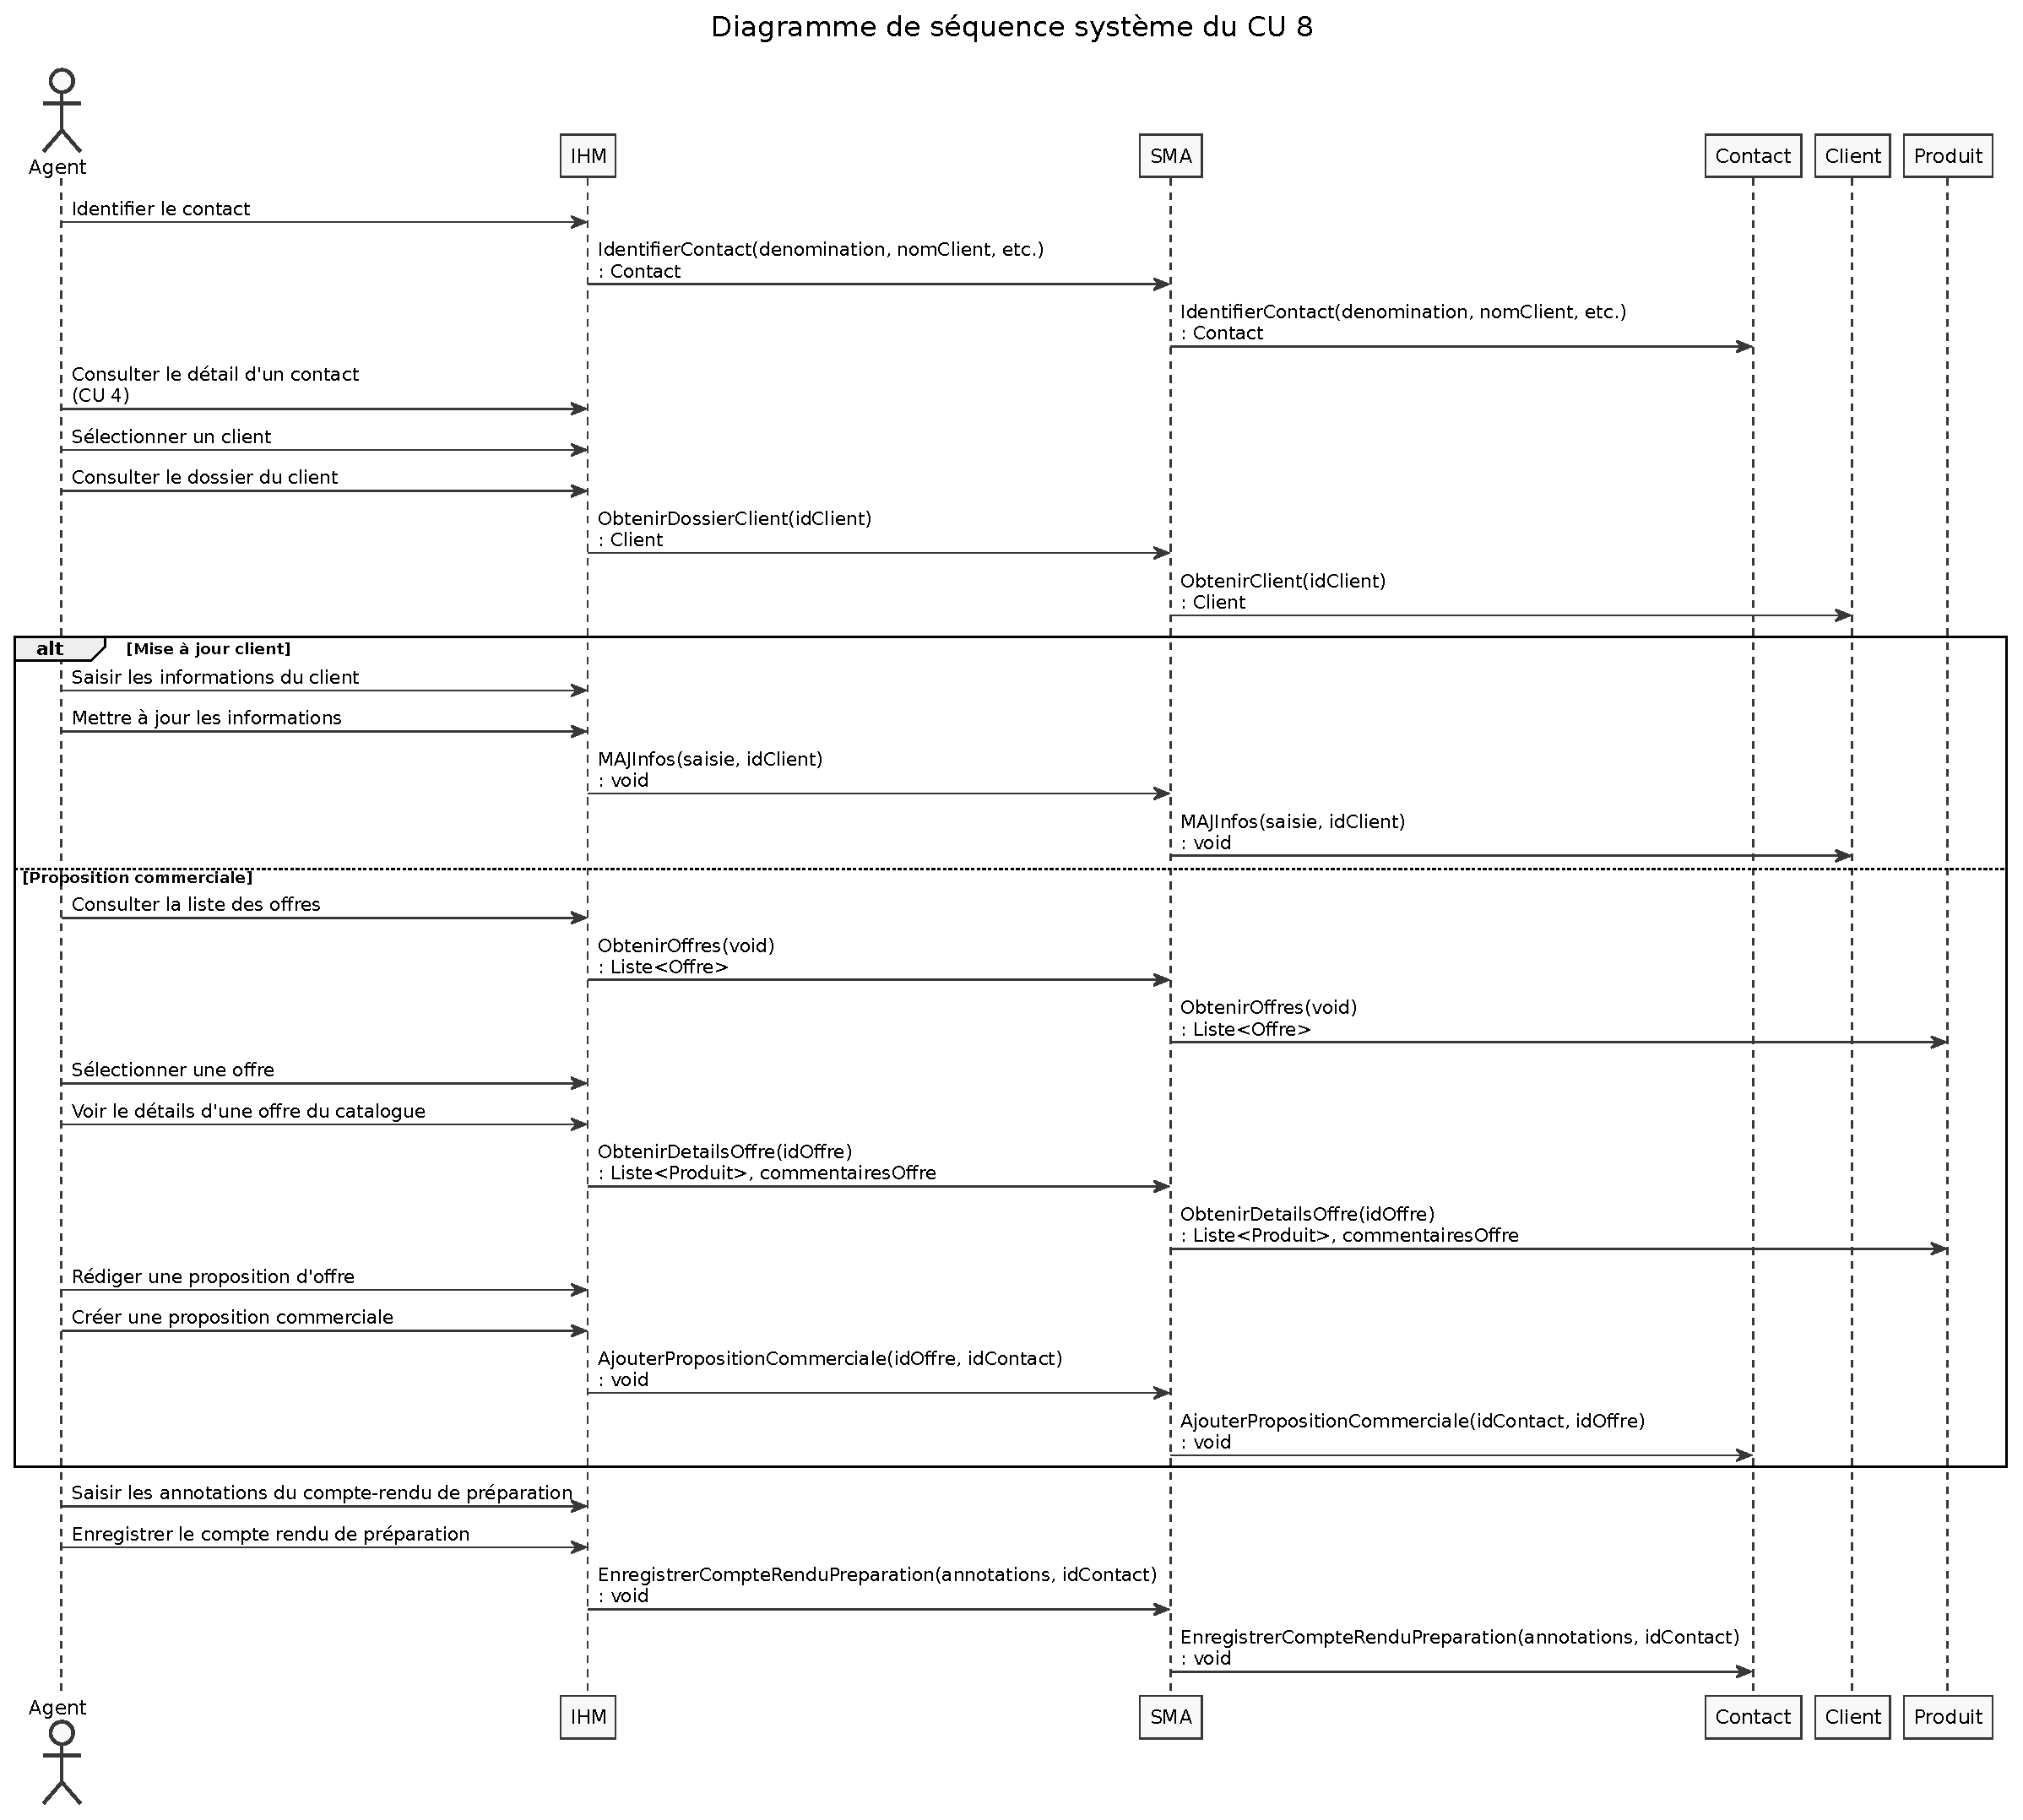
\includegraphics[width=22cm, angle=90]{figures/eps/DSD_CU8.eps}}
\caption{DSD du CU8}
\end{figure}

\subsection{CU9 - Conduite de l’entretien par l’agent}
\begin{figure}[H]
\noindent\makebox[\textwidth]{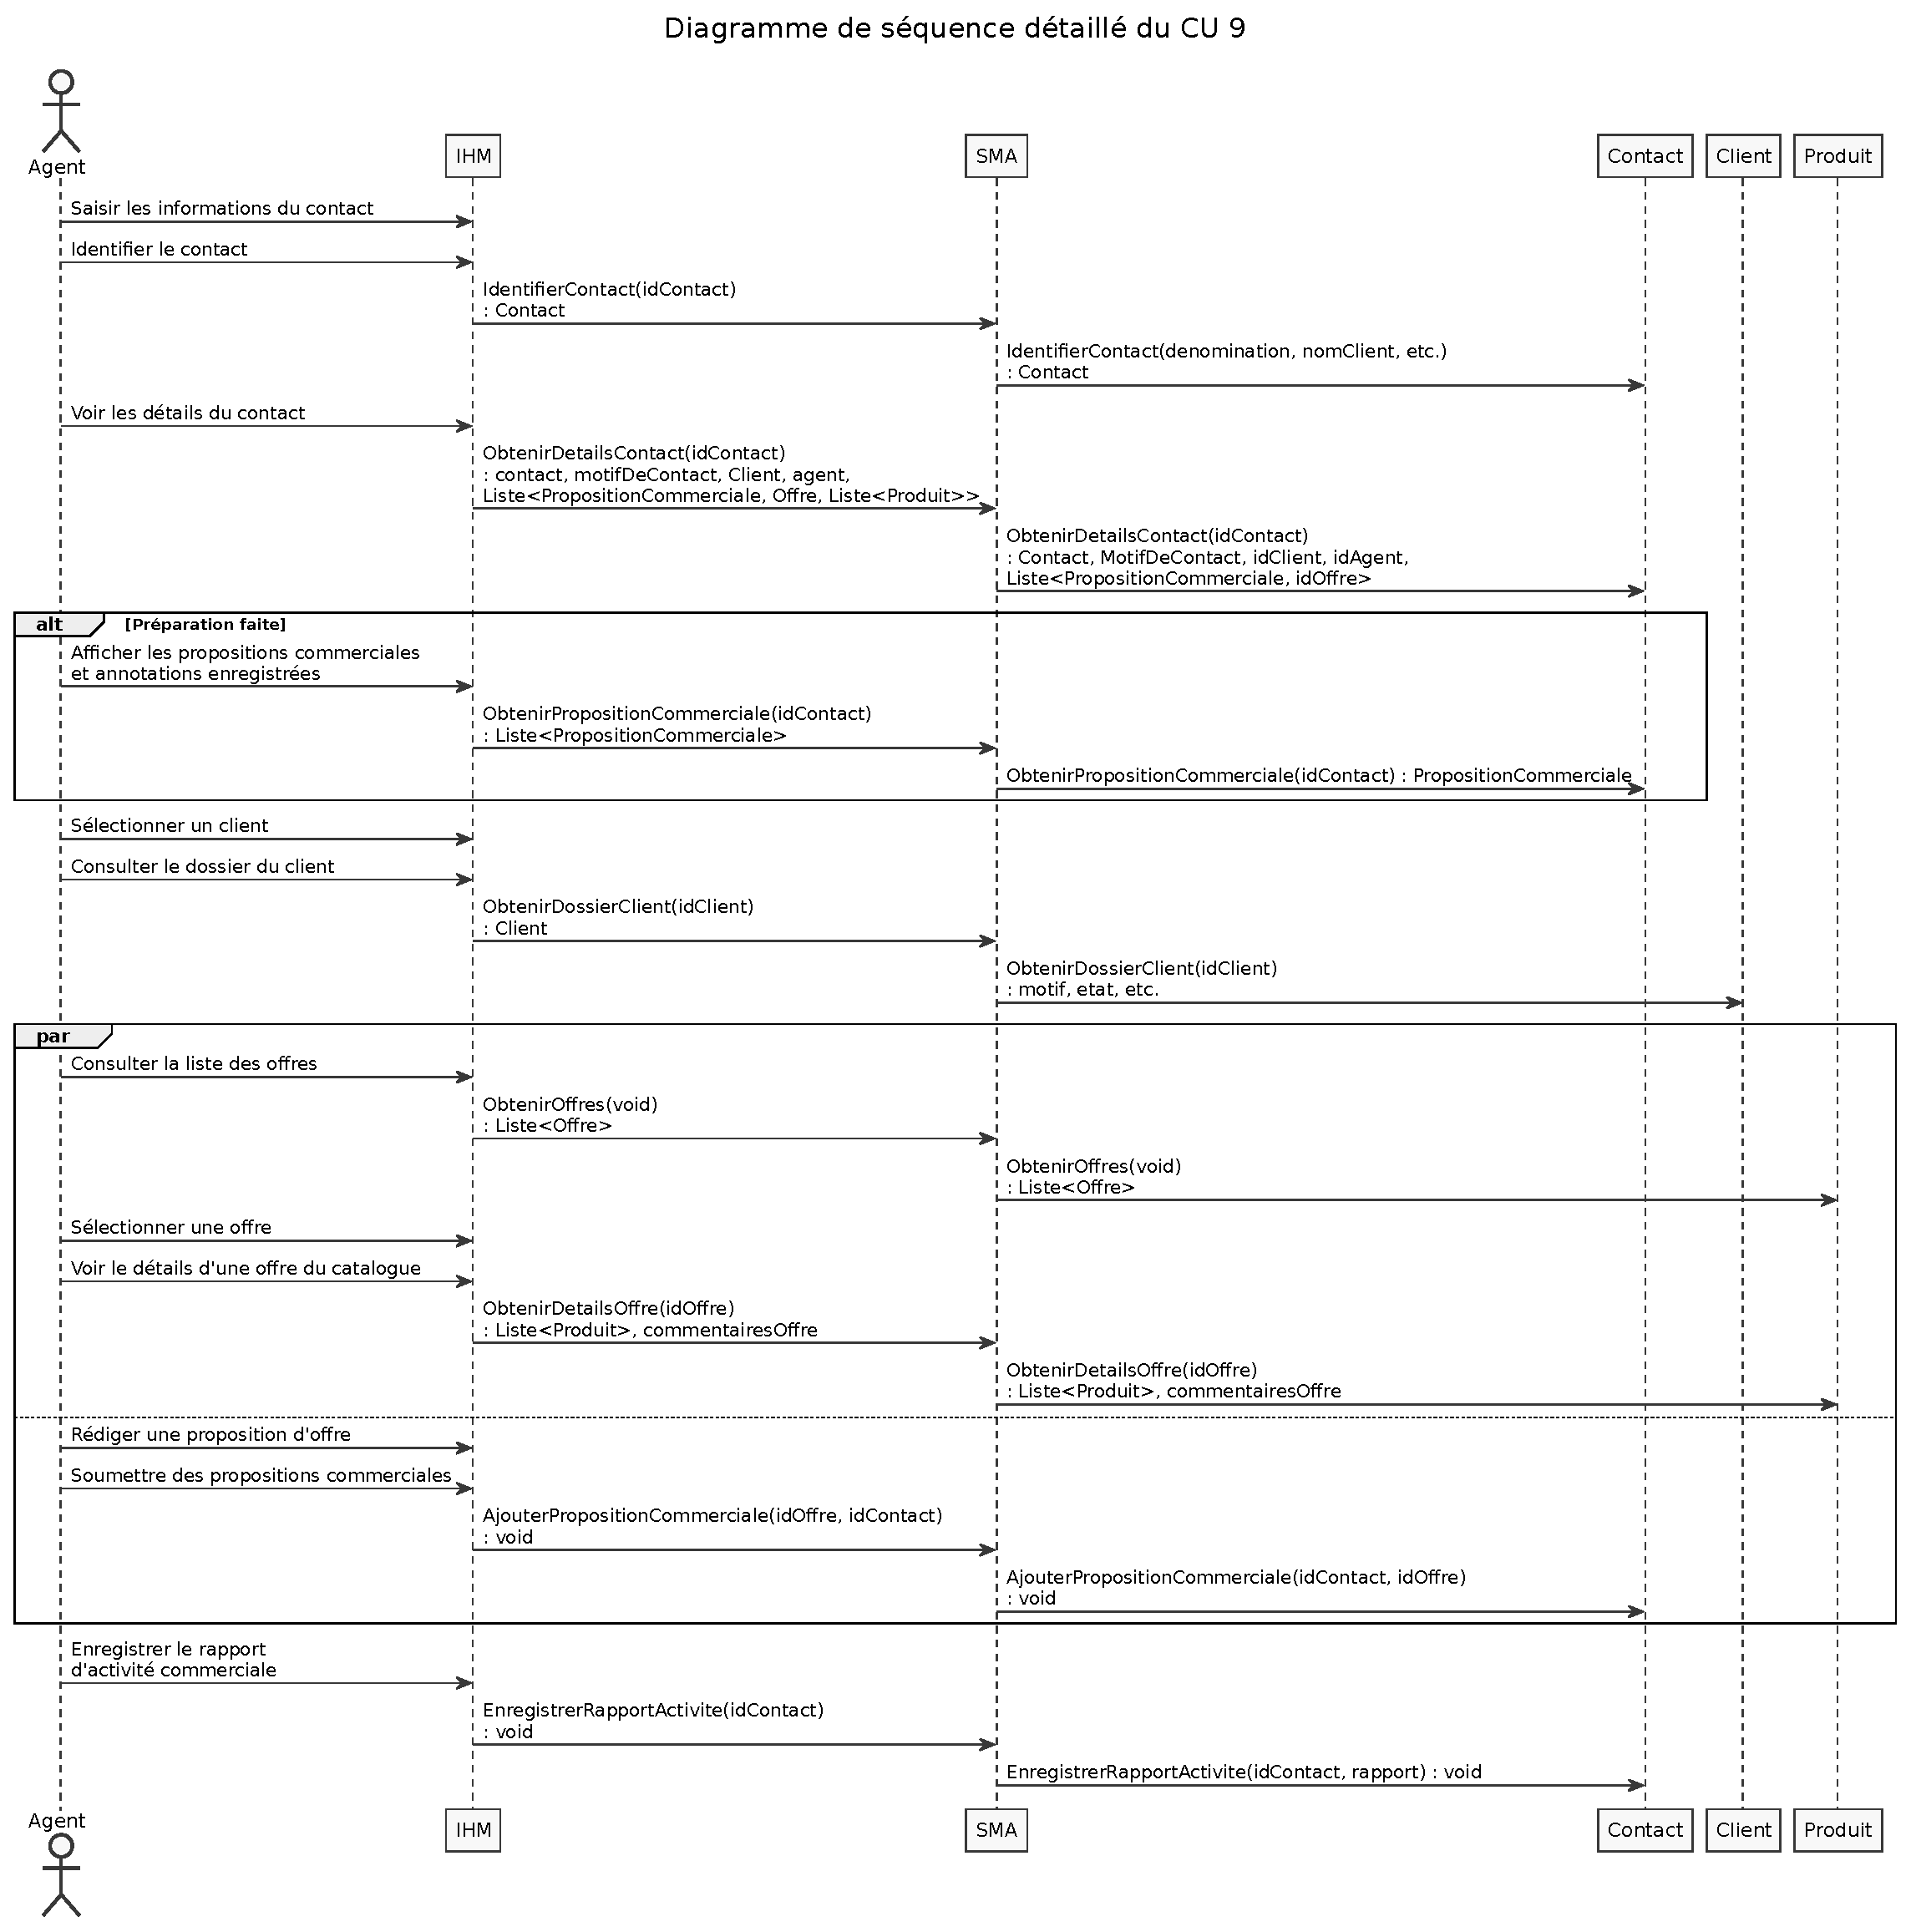
\includegraphics[width=19.5cm, angle=90]{figures/eps/DSD_CU9.eps}}
\caption{DSD du CU9}
\end{figure}

\subsection{CU10 - Consultation du dossier client}
\begin{figure}[H]
\noindent\makebox[\textwidth]{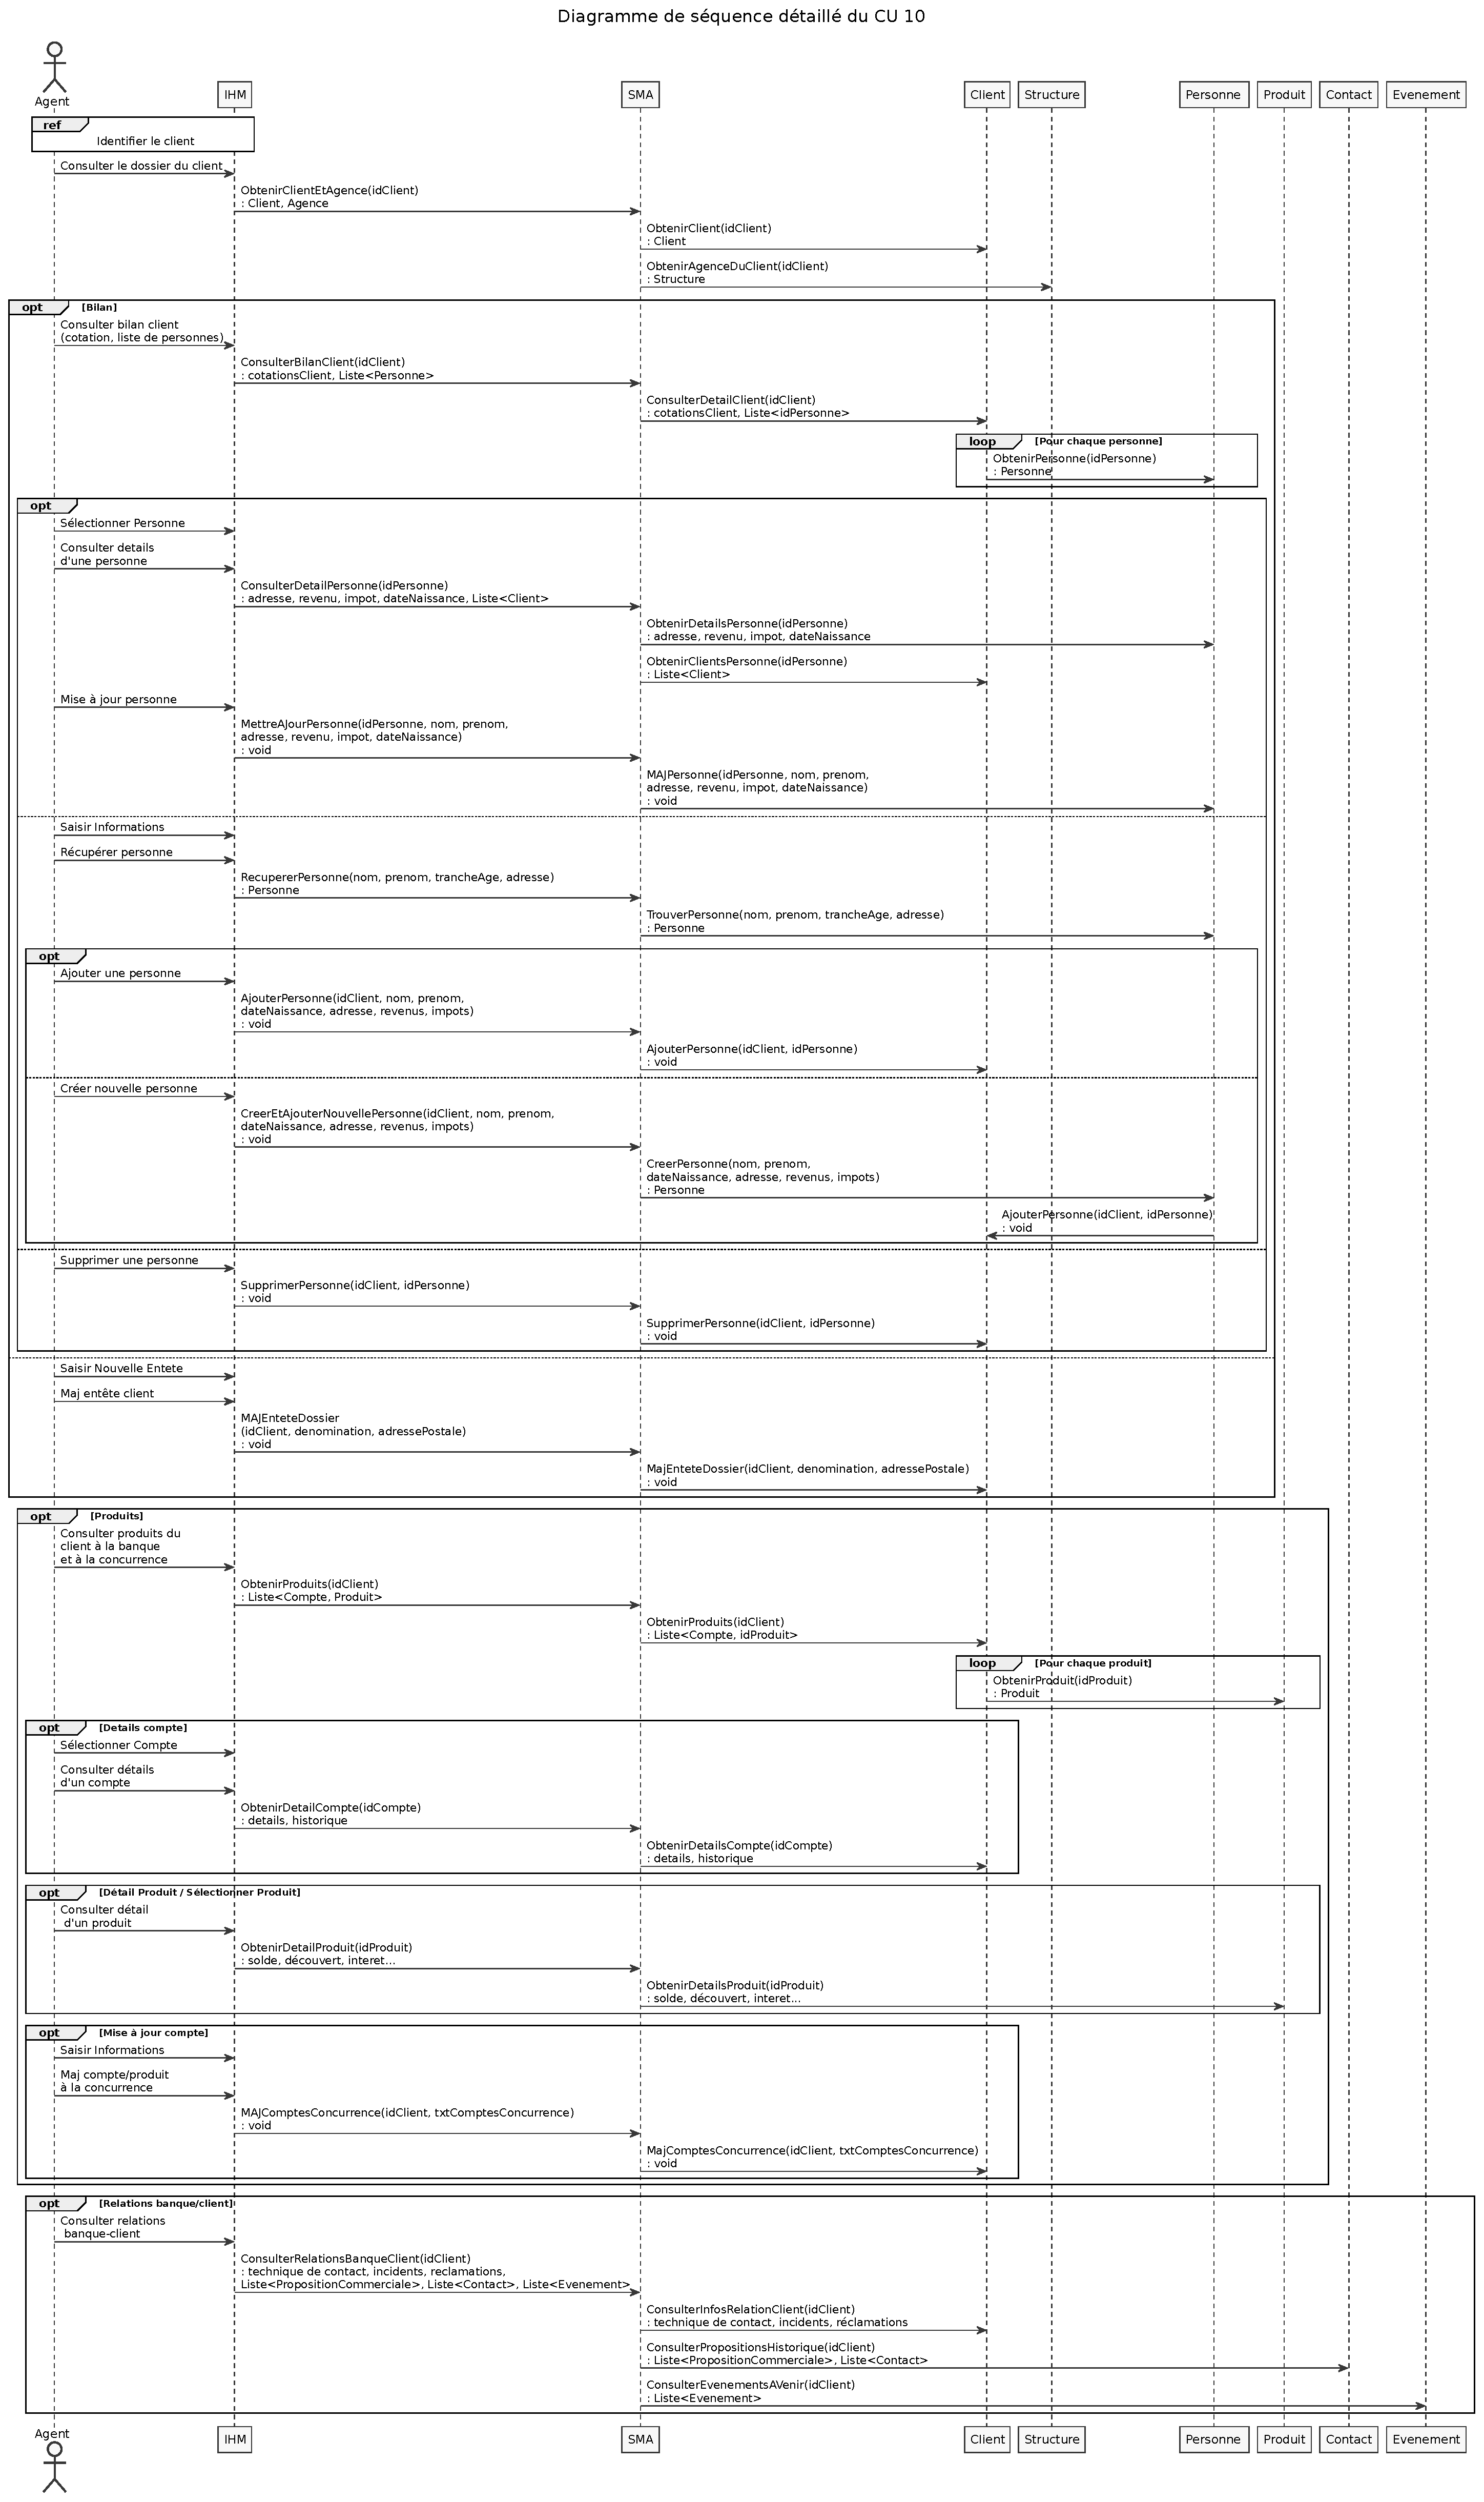
\includegraphics[width=14.2cm]{figures/eps/DSD_CU10.eps}}
\caption{DSD du CU10}
\end{figure}


\newgeometry{height=10in}.
\section{Spécification des services}
\subsection{SMA : ObtenirAgendaAgent(idAgent, numSemaine, annee)}
Ce service métier applicatif permet d'obtenir le détail des activités et tâches élémentaires d'un agent pour une semaine en particulier, tout en détaillant les plages horaires associées, permettant ainsi d'obtenir son agenda hebdomadaire. \\

\noindent \textit{\textit{Arguments en entrée :}}
\begin{description}
\item[idAgent] l'identifiant numérique de  l'agent pour lequel on souhaite obtenir l'agenda. 
\item[numSemaine] le numéro de la semaine à rechercher, de 1 à 52. 
\item[annee] l'année pour laquelle on souhaite obtenir l'agenda de la semaine mentionnée en second argument, sous format numérique, à quatre chiffres. \\
\end{description}

\noindent \textit{Sorties} :

\begin{description}
\item[Agent] l'agent associé à l'identifiant passé en premier paramètre.
\item[Liste<PlageAgenda, TypeActivite, Liste<TacheElementaire, Client>>] l'ensemble des plages agenda de l'agent ayant l'identifiant idAgent, pour la semaine numSemaine de l'année annee, avec les activités et les tâches élémentaires associées. Pour chaque tâche élémentaire, le client correspondant est également retourné, permettant ainsi d'obtenir les informations générales sur ce dernier. \\
\end{description}

\begin{shaded}
\textbf{SOM associés}\\
\textbf{1.} : Dans un premier temps, le bloc Agenda est interrogé, permettant de retourner les plages agenda, les activités ainsi que les tâches élémentaires associées à l'identifiant agent passé en paramètre. Le SOM correspondant est le suivant : 
\end{shaded}

\subsubsection{ObtenirAgendaAgent(idAgent, numSemaine, annee)}

\noindent \textit{Argument en entrée :}
\begin{description}
\item[idAgent] l'identifiant numérique de l'agent pour lequel on souhaite obtenir l'agenda. 
\item[numSemaine] le numéro de la semaine à rechercher, de 1 à 52. 
\item[annee] l'année pour laquelle on souhaite obtenir l'agenda de la semaine mentionnée en second argument, sous format numérique, à quatre chiffres. \\
\end{description}

\noindent \textit{Sorties} :
\begin{description}
\item[Liste<PlageAgenda, TypeActivite, Liste<TacheElementaire, idContact>>] la liste des plage agenda, des types d'activité et des tâches élémentaires associées. Pour chaque tâche élémentaire retournée, l'identifiant du contact associé est également retourné, permettant ainsi de récupérer le contact en interrogeant le bloc Contact par la suite. \\
\end{description}

\begin{shaded}
\textbf{2.} : Après avoir obtenu une tâche élémentaire grâce au bloc Agenda, le bloc Contact est interrogé afin d'obtenir l'identifiant du client qui est concerné par la plage horaire que l'on souhaite décrire. Le SOM ci-dessous nous permet d'obtenir cet identifiant.
\end{shaded}

\subsubsection{ObtenirClientDuContact(idContact)}

\noindent \textit{Argument en entrée :}
\begin{description}
\item[idContact] l'identifiant du contact à rechercher dans le bloc Contact, qui a été retourné dans notre cas par le SOM ObtenirAgendaAgent \\
\end{description}

\noindent \textit{Sortie} :
\begin{description}
\item[idClient] l'identifiant du client associé au contact, permettant par la suite d'obtenir l'entité client correspondante en interrogeant le bloc Client. \\
\end{description}

\begin{shaded}
\textbf{3.} : Enfin, le bloc Client est interrogé afin d'obtenir l'entité éponyme, associée à l'identifiant obtenu grâce au SOM précédent.
\end{shaded}

\subsubsection{ObtenirClient(idClient)}

\noindent \textit{Argument en entrée :}
\begin{description}
\item[idClient] l'identifiant du client à rechercher dans le bloc Client, qui a été retourné dans notre cas par le SOM ObtenirClientDuContact. \\
\end{description}

\noindent \textit{Sortie} :
\begin{description}
\item[Client] l'entité client correspondant à l'identifiant passé en paramètre. \\
\end{description}

\subsection{SMA : ObtenirDetailsRdv(idTacheElementaire)} 

Ce service métier applicatif permet de retourner les informations détaillées d'un rendez-vous associé à une tâche élémentaire spécifique.\\

\noindent \textit{Argument en entrée :}
\begin{description}
\item[idTacheElementaire] l'identifiant de la tâche élémentaire qui représente le rendez-vous que l'on souhaite détailler. \\
\end{description}

\noindent \textit{Sorties} : 
\begin{description}
\item[TacheElementaire] la tâche élémentaire associée à l'identifiant passé en paramètre.
\item[PlageAgenda] la plage agenda associée à la tâche élémentaire également retournée.
\item[Agent] l'agent associé à la plage agenda retournée et, de fait, associé au rendez-vous que l'on souhaite détailler. 
\item[Contact] le contact qui est associé à la plage agenda retournée et qui doit être (ou à été) réalisé durant ce créneau horaire.
\item[MotifDeContact] le motif du contact de la plage agenda possédant l'identifiant passé en paramètre. 
\item[Client] le client concerné par le rendez-vous. \\
\end{description}


\begin{shaded}
\textbf{SOM associés}\\
\textbf{1.} Dans un premier temps, le bloc Agenda est interrogé, ce dernier possédant les informations les plus importantes pour ce SMA, ce dernier étant relatif à une plage agenda, qui est une entité de ce bloc. Le service objet métier ci-dessous.
\end{shaded}


\subsubsection{ObtenirDetailsRdv(idTacheElementaire)}

\noindent \textit{Argument en entrée :}
\begin{description}
\item[idTacheElementaire] l'identifiant de la tâche élémentaire qui représente le rendez-vous à détailler. \\
\end{description}

\noindent \textit{Sorties} : 
\begin{description}
\item[TacheElementaire] la tâche élémentaire présente dans le bloc Agenda, qui correspond à l'identifiant passé en paramètre.
\item[PlageAgenda] la plage agenda présente dans le bloc Agenda, qui correspond à la tâche élémentaire également retournée.
\item[idAgent] l'identifiant de l'agent associé à la plage agenda, qui sera utilisé pour retrouver l'agent dans le bloc Structure. 
\item[idContact] l'identifiant du contact associé à la page agenda, qui sera utilisé pour retourner le contact et le motif de contact. \\
\end{description}

\begin{shaded}
\textbf{2.} Afin d'obtenir les détails associés au contact relié à la tâche élémentaire récupérée dans le bloc Agenda, le bloc Contact est interrogé grâce à l'identifiant contact connu dans le bloc Agenda. Le service objet entier utilisé est le suivant :
\end{shaded}

\subsubsection{ObtenirResumeContact(idContact)}

\noindent \textit{Argument en entrée :}
\begin{description}
\item[idContact] l'identifiant du contact pour lequel on souhaite obtenir les informations détaillées. \\
\end{description}

\noindent \textit{Sorties} :
\begin{description}
\item[Contact] l'entité contact possédant l'identifiant passé en paramètre. 
\item[MotifDeContact] le motif de contact associé à l'entité contact qui possède l'identifiant passe en paramètre.  
\item[idClient] l'identifiant du client qui est rattaché à l'entité contact retournée, permettant d'obtenir par la suite plus d'informations sur le client via le bloc Client. 
\item[idAgent] l'identifiant de l'agent qui est rattaché au contact, permettant si besoin est de récupérer l'entité associée dans le bloc Structure par la suite. \\
\end{description}

\begin{shaded}
\textbf{3.} Le bloc Contact ayant permis d'obtenir l'identifiant client associé au contact relié au rendez-vous que l'on souhaite détailler, le bloc Client est ensuite interrogé grâce au service métier suivant :
\end{shaded}

\subsubsection{ObtenirClient(idClient)}

\noindent \textit{Argument en entrée :}
\begin{description}
\item[idClient] l'identifiant du client pour lequel on souhaite obtenir plus d'informations. \\
\end{description}


\noindent \textit{Sortie} :
\begin{description}
\item[Client] l'entité client associée à l'identifiant passée en paramètre et qui correspond au client concerné par le rendez-vous.\\
\end{description}

\begin{shaded}
\textbf{4.} Le bloc Contact permettant également d'obtenir l'identifiant de l'agent concerné par le rendez-vous, le service objet métier ci-dessous, du bloc Structure, est ensuite appelé. 
\end{shaded}


\subsubsection{ObtenirAgent(idAgent)}

\noindent \textit{Argument en entrée :}
\begin{description}
\item[idAgent] l'identifiant de l'agent qui s'occupe du rendez-vous que l'on souhaite détailler. \\
\end{description}

\noindent \textit{Sortie} :
\begin{description}
\item[Agent] l'entité agent associé à l'identifiant passé en paramètre et trouvé dans le bloc Structure. \\
\end{description} 


\restoregeometry
\subsection{Listes complètes des services}

\begin{table}
    \centering
    \scalebox{0.8}{
        \begin{tabular}{p{1cm}|p{5cm}p{6cm}p{6cm}}
        Numéro SM & Nom & Arguments & Valeur de retour \\ \hline
        1  & GenererContacts                    & void                                                          & void \\ \hline
        2  & ObtenirContactsPrevus              & idAgence                                                      & Liste <Contact> \\ \hline
        3  & ObtenirDetailsContact              & idContact                                                     & contact, motifDeContact, client, agentListe<PropositionCommerciale>, Liste<Offre>, Liste<Produit>\\ \hline
        4  & ObtenirDossierClient               & idClient                                                      & Client\\ \hline
        5  & ObtenirAgents                      & idAgence                                                      & Liste<Agent>\\ \hline
        6  & ObtenirDetailsAgent                & idAgent                                                       & agent, Liste<ContactPrevu>\\ \hline
        7  & AffecterContact                    & idContact, idAgent                                            & void\\ \hline
        8  & ObtenirContactsAgent               & idAgent                                                       & Liste<Contact>\\ \hline
        9  & ObtenirContactsATraiter            & idAgent                                                       & Liste<ContactRealise>\\ \hline
        10 & GrouperContacts                    & idContactPrincipal, Liste<idContactPrevus>                    & void\\ \hline
        11 & EnregistrerMotifAnnulation         & idContact, motif                                              & void\\ \hline
        12 & AnnulerContact                     & idContact                                                     & void\\ \hline
        13 & PrendreRdv                         & idContact                                                     & void\\ \hline
        14 & PreparerRdv                        & idContact                                                     & void\\ \hline
        15 & ConduireRdv                        & idContact                                                     & void\\ \hline
        16 & ObtenirAgendaAgent                 & idAgent, numSemaine, annee                                    & Liste<PlageAgenda>, Liste<TacheElementaire>, Liste<TypeActivite> \\ \hline
        17 & ReaffecterRdv                      & idPlageAgenda, idAgent                                        & void\\ \hline
        18 & ObtenirDetailsRdv                  & idPlageAgenda                                                 & plageAgenda, agent, contactRealise,  contactPrevu, motifDeContact, client\\ \hline
        19 & ModifierPlageHoraire               & idPlageAgenda, plageHoraireDeb, plageHoraireFin               & plageAgenda\\ \hline
        20 & ObtenirAgendaAgence                & idAgence, dateJour                                            & Liste<PlageAgenda>, Liste<TacheElementaire>,  Liste<TypeActivite>\\ \hline
        21 & AnnulerRdv                         & idPlageAgenda                                                 & void\\ \hline
        22 & CreerPlageAgenda                   & idAgent, idActivite, datePlageHoraireDeb, datePlageHoraireFin & plageAgenda\\ \hline
        23 & MajNbContactsPotentiels            & idAgent, Liste<idPlageAgenda>                                 & void\\ \hline
        24 & IdentifierContact                  & idContact                                                     & Contact\\ \hline
        25 & MAJInfos                           & saisie, idClient                                              & void\\ \hline
        26 & ObtenirOffres                      & void                                                          & Liste<Offre>\\ \hline
        27 & ObtenirDetailsOffre                & idOffre                                                       & Details\\ \hline
        28 & AjouterPropositionCommerciale      & idOffre, idContact                                            & void\\ \hline
        29 & EnregistrerCompteRenduPreparation  & idContact                                                     & void\\ \hline
        30 & ObtenirPropositionCommerciale      & idContact                                                     & Liste<PropositionCommerciale>\\ \hline
        31 & EnregistrerRapportActivite         & idContact                                                     & void\\ \hline
        32 & ConsulterDossierClient             & idClient                                                      & numero, denomination, adresse postale\\ \hline
        33 & ConsulterBilanClient               & idClient                                                      & cotationsClient, liste Personnes\\ \hline
        34 & ConsulterDetailPersonne            & idPersonne                                                    & données signalétiques...logement\\ \hline
        35 & MettreAJourPersonne                & idPers,...                                                    & void\\ \hline
        36 & RecupererPersonne                  & nom, prenom, agence                                           & personne\\ \hline
        37 & AjouterPersonne                    & idClient, idPersonne                                          & void\\ \hline
        38 & CreerEtAjouterNouvellePersonne     & infos, idClient                                               & personne\\ \hline
        39 & SupprimerPersonne                  & idClient, idPersonne                                          & void\\ \hline
        40 & MAJEnteteDossier                   & idClient, numero, denomination, adressePostale                & void\\ \hline
        41 & ObtenirDetailCompte                & idCompte                                                      & details, historique\\ \hline
        42 & ObtenirDetailProduit               & idProduit                                                     & details\\ \hline
        43 & ObtenirProduits                    & idClient                                                      & Liste<Compte, Produit>\\ \hline
        44 & MAJComptesConcurrence              & idClient, txtComptesConcurrence                               & void \\ \hline
        45 & ObtenirPlagesLibres                & idAgent                                                       & Liste<PlageAgenda>\\ \hline
        46 & AssocierPlageEtContact             & idPlage, idContact                                            & void\\ \hline
        47 & EnregistrerLettreConfirmationRdv   & idContactRealise, lettre                                      & void\\ \hline
        48 & RechercherClient                   & prenom, nom, etc                                              & client\\ \hline
        49 & CreerContactSpontane               & idClient, idAgent, motifContact                               & contactPrevu, contactRealise\\ \hline
        50 & CreerRDVSpontane                   & idContactRealise, date, commentaire                           & plageAgenda\\ 
        \end{tabular}
        }
        \caption{Tableau de synthèse des SMA}
\end{table}

\begin{table}
    \centering
    \begin{tabular}{l|l}
    Nom de la vue   & Numéros des SMA appelés   \\ \hline
    ~               & ~                         \\ 
    \end{tabular}
    \caption{Tableau de synthèse des SMA par fenêtre}
\end{table}





\part{Architecture technique et répartition du système d’information}

\newgeometry{height=10in}.

Cette section présente les choix techniques effectués dans le cadre de la conception de l'architecture technique.

\section{Choix du type d'IHM}

Nous avons choisi de concevoir un client léger sous forme d'une application web. Nous avons réalisé ce choix après considération de différents critères. Il nous semble plus facile de maintenir une application centralisée putôt qu'une application distribuée. En effet, dès qu'une mise à jour de l'application est réalisée, il est plus simple de mettre à jour l'application sur quelques serveurs que sur plusieurs centaines de postes clients. Cette application ne pouvant être utilisée hors ligne, un client lourd ne présente pas plus d'intérêt selon ce critère. Il est également important de prendre en compte le fait que le client lourd implique une grande quantité de travail pour l'adapter à des environnements différents tandis qu'un simple navigateur à jour permettra d'accèder à l'application. En effet, même si ce client lourd est développé dans un langage permettant la portabilité du code, il nécessitera l'installation de dépendances pour son fonctionnement ce qui n'est pas viable à long terme et implique des coûts importants en termes de ressources. 

\section{Serveurs et localisation}

La répartition des serveurs présentée dans la suite fait référence à la figure suivante présentant le diagramme d'organisation fourni dans le sujet.

\begin{figure}[H]
    \centering
	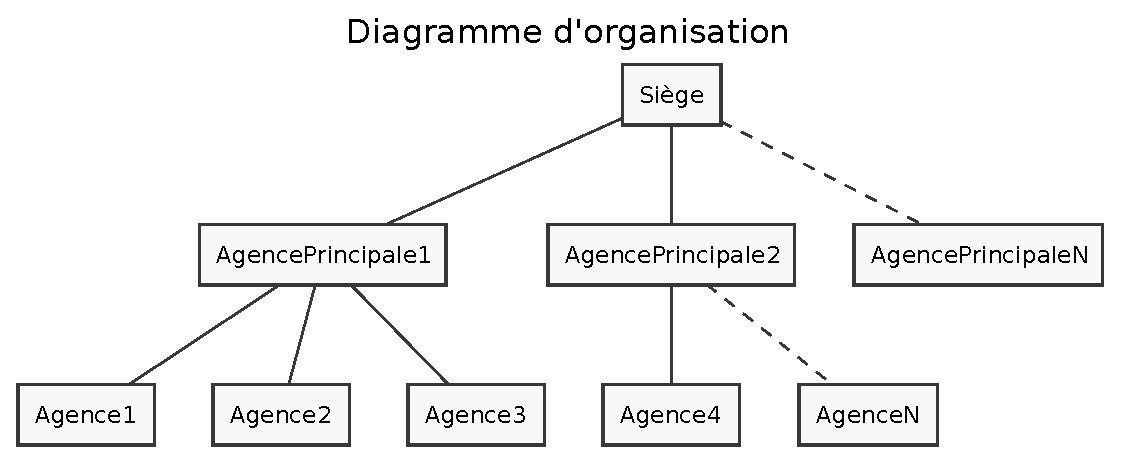
\includegraphics[scale=0.6]{figures/eps/DO}
	\caption{Diagramme d'organisation}
\end{figure}

Nous avons répartis les serveurs de données en répondant aux questions suivantes :\\
\begin{itemize}
	\item[\textbullet] La donnée est-elle partagée ? Si oui, par qui ?
	\item[\textbullet] Quelle est la fréquence d'accès à la donnée ?
	\item[\textbullet] En terme de sécurité, qui a besoin d'accéder à la donnée ?\\
\end{itemize}

Nous avons donc abouti à une répartition optimale selon nos critères. Des serveurs de données seront implantés au siège (site central) ainsi que dans les agences principales mais pas dans les agences rattachées aux agences principales. \'Etant donné le fait que la gestion des données clients et produits est réalisée au siège, celui-ci nécessite évidemment des serveurs pour stocker ces données. Ensuite, il nous semble réaliste de distribuer la donnée propre à chaque agence au sein de l'angence principale à laquelle elle est rattachée. Cela permettra de ne pas surcharger d'information inutile les entités ne nécessitant pas l'accès à ces données. De plus, cela aura un effet important sur les performances globales du système et notamment la diminution du nombre de requêtes sur des sites distants qui aura pour effet de réduire les temps de réponse. Il nous semble par contre irréaliste de déployer un serveur de données par agence, ce qui entrainerait des coûts de maintenance non négligeables.\\

Nous avons procédé de la même manière concernant les serveurs d'applications en nous posant des questions différentes :\\
\begin{itemize}
	\item[\textbullet] Est-il possible et intéressant, étant donnée la répartition des serveurs de données, de distribuer les composants applicatifs ?
	\item[\textbullet] Quelles seraient les conséquences d'un tel déploiement ?\\
\end{itemize}

Nous sommes donc arrivés aux conclusions suivantes. Afin de profiter des avantages offerts par le client léger, nous ne devons pas trop répartir les serveurs d'applications et il n'est donc pas souhaitable d'équiper chaque agence d'un serveur d'applications. Il n'est pas non plus intéressant d'équiper seulement le siège d'un serveur d'application, en particulier si l'on considère la charge qu'il subira si toutes les agences font appel à ce serveur central. Il est également important de noter qu'en cas de dysfonctionnement du serveur d'application sur le site central, toutes les agences seront impactées. Il semble donc judicieux d'équiper chaque agence principale d'un serveur d'application. En effet, cela apporte de nombreux avantages. Parmis ceux-ci le fait de pouvoir déployer progressivement une nouvelle version d'un applicatif ce qui est pratiqué dans beaucoup de grands groupes avec des entités qui réalisent les tests des nouvelles versions sans impacter l'intégralité des agences jusqu'à la validation de la version. Cette répartition augmente également la tolérance aux pannes et réduit la charge réseaux induite par les postes clients. Un serveur d'applications devra tout de même être présent au siège pour supporter les composants applicatifs partagés.\\

Le tableau ci-dessous présente la synthèse de nos choix concernant la répartition des serveurs et le nombre de serveurs à implanter. Ces choix seront renforcés par les choix concernant la répartition des blocs applicatifs et les flux de données induits par cette architecture. 


\begin{table}[H]
    \centering
    \begin{tabular}{l|l|l}
    Type d'entité        & Serveur de Données & Serveur d'Applications \\ \hline
    Siège (site central) & Oui ($n$)            & Oui ($n$)                \\
    Agence principale    & Oui ($1$)            & Oui ($1$)                \\
    Agence simple        & Non                & Non                    \\
    \end{tabular}
    \caption{Tableau de répartition des serveurs par entité organisationnelle}
\end{table}

\section{Implantation des composants du noyau applicatif et flux de données}

Etant donnée la répartition des serveurs précédemment exposée et la contrainte concernant la gestion des données client et produit nous avons jugé qu'il serait intéressant de déployer les blocs applicatifs Personne, Client, Produit et Structure sur le(s) serveur(s) d'applications situé(s) sur le site central. Il semble également envisageable de distribuer les composants Contact et Agenda sur les serveurs d'applications respectifs des différentes agences principales. Il pourrait être avantageux de répliquer les données concernant les clients et les structures au niveau des agences principales. \\

Si nous considérons les flux de données, relatifs à des opérations classiques, induits par ces différents choix nous obtenons les résultats suivants. Une opération de consultation ou d'édition de l'agenda ne ferait intervenir que les serveurs situés au niveau de l'agence. Seules les opérations liées aux clients ou aux produits feront intervenir les serveurs du site central. Enfin, la réplication des clients concernant une agence rattachée à une agence principale permettrait de gérer les évènements concernant les clients au niveau des agences principales également.
Du point de vue de la sécurité du système il est également intéressant de noter que la répartition choisie permet une bonne segmentation des données. Par exemple, la corruption d'un système au niveau d'une agence principale ne permettrait pas d'accèder aux agendas de toutes les agences ni à la liste de tous les clients. De même, les informations confidentielles concernant les clients seront toutes stockées au siège ce qui permettra une protection efficace de ces dernières. Dans le cas d'une corruption de ce système central, l'attaquant ne sera pas forcément en mesure de consulter les agendas des agences. Cette architecture nécessite par contre des protections adéquates des communications entre les différents systèmes distribués.

Le tableau ci-dessous présente la synthèse de nos choix concernant la répartition des composants sur l'architecture physique. 

\begin{table}[H]
    \centering
    \begin{tabular}{l|l|l|l|l|l|l}
    Type d'entité        & Personne & Client   & Produit & Structure & Contact & Agenda \\ \hline
    Siège (site central) & Oui      & Oui      & Oui     & Oui       & Non     & Non    \\
    Agence principale    & Non      & Répliqué & Non     & Répliqué  & Oui     & Oui    \\
    Agence simple        & Non      & Non      & Non     & Non       & Non     & Non    \\
    \end{tabular}
    \caption{Tableau de répartition des objets métiers par entité organisationnelle}
\end{table}

La figure suivante présente la répartition des serveurs, la répartition des blocs et les flux de données.

\begin{figure}[H]
    \centering
    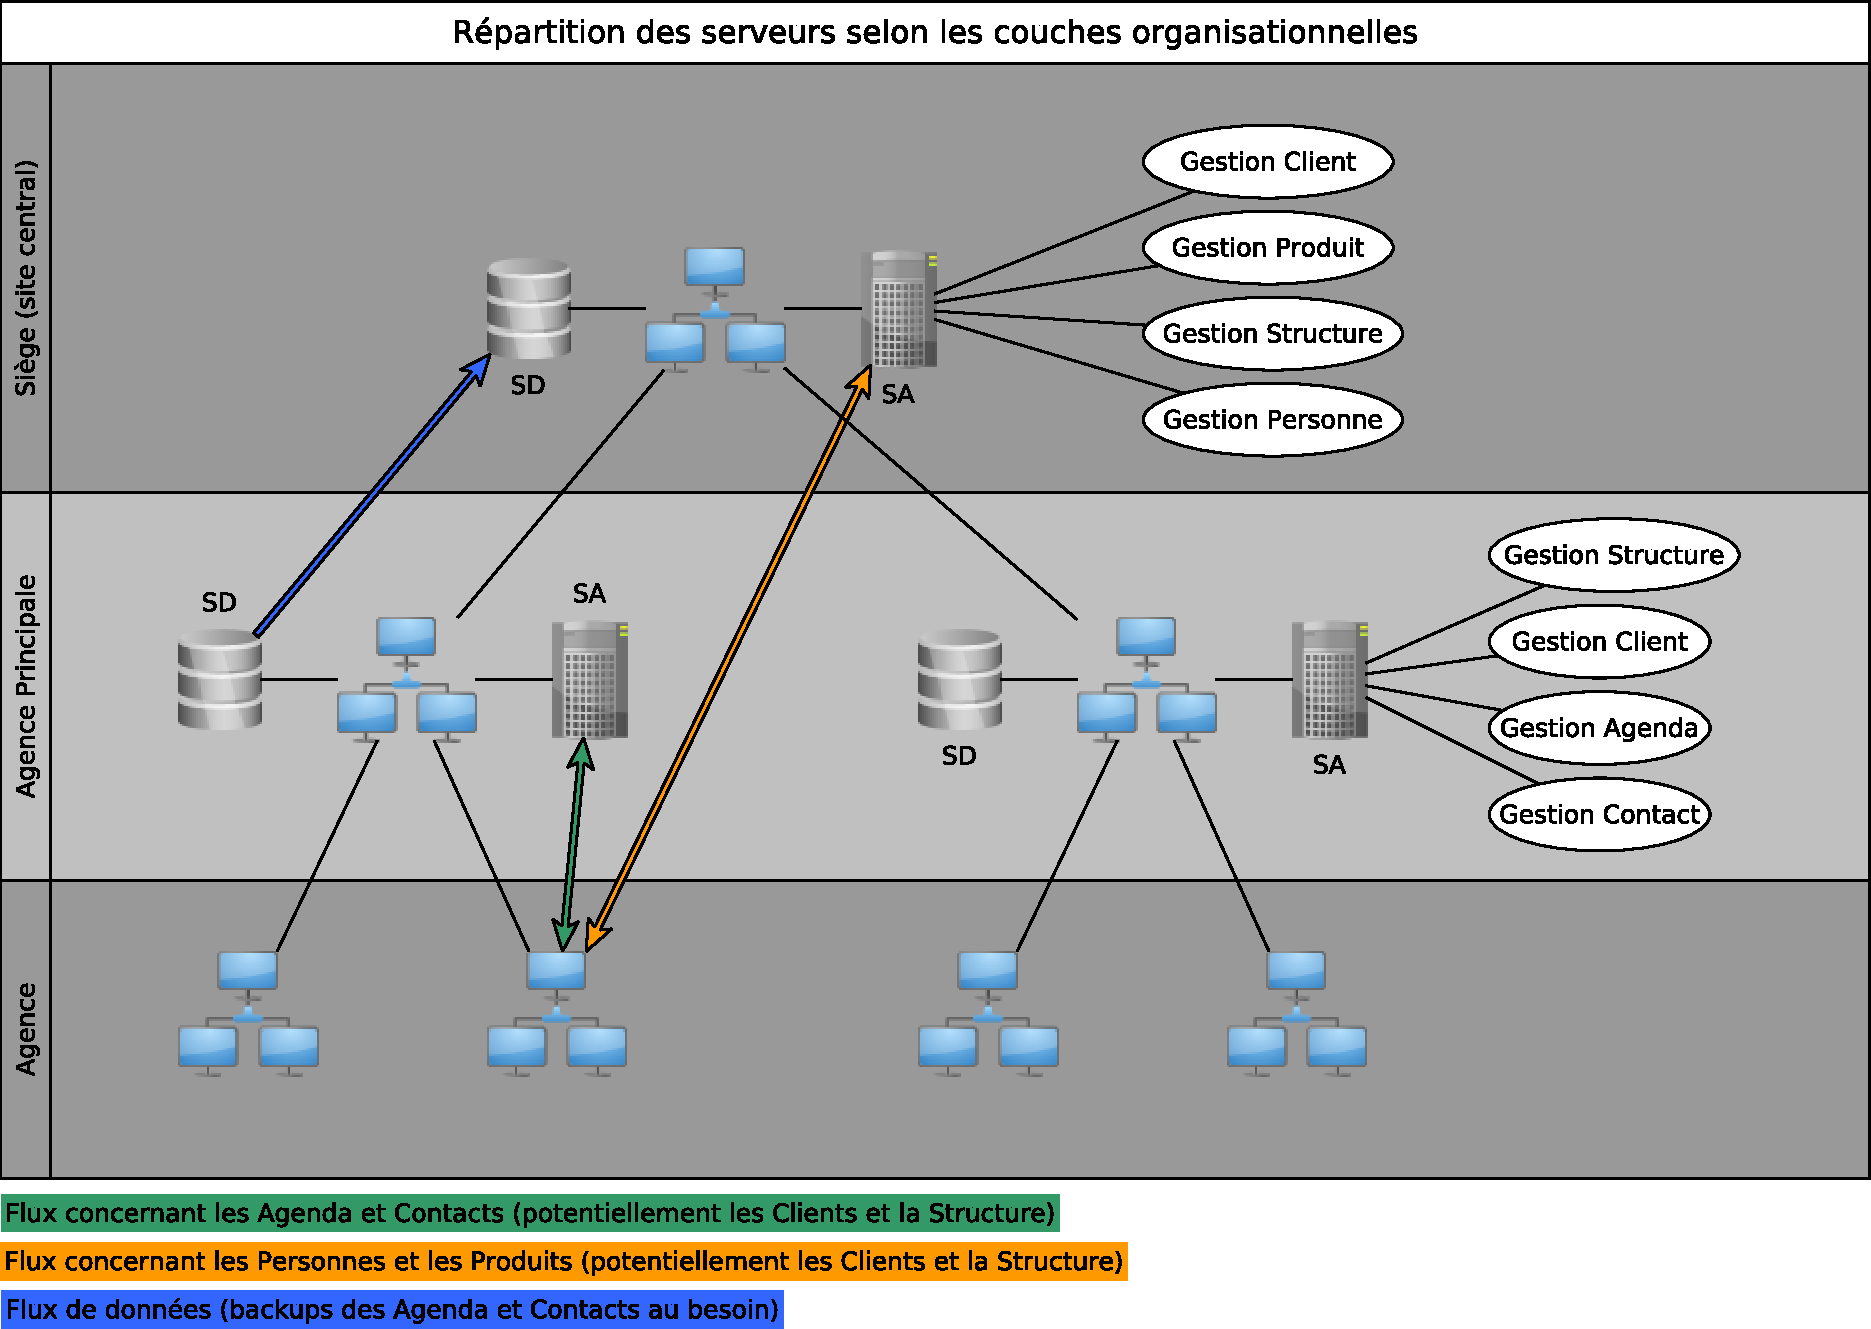
\includegraphics[scale=0.5]{figures/architectureServeurs.pdf}
    \caption{Plan de répartition des serveurs}
\end{figure}


\restoregeometry

\part{Diagramme de collaboration - Validation de l'architecture globale}
\setcounter{section}{0}

\section{Diagramme de collaboration}

\todo[inline]{insérer dagramme de collaboration}
\part{Conclusion et Bilan}
\setcounter{section}{0}

\newgeometry{height=10in}.

\section{Bilan du chef de projet}

\subsection{Bilan global}
Le projet s'est dans l'emsemble bien déroulé. Le principal problème de ce projet a été de constamment devoir recommencer les différents diagrammes jusqu'à ce qu'ils soient corrects. De plus, il existe peu d'outils qui soient réellement pratiques pour la réalisation de ces projets, surtout en ce qui concerne les IHM.

\subsection{Outils utilisés}
Dans le but d'harmoniser l'ensemble du rendu, nous avons choisi d'utiliser \textbf{PlantUML} pour réaliser l'ensemble des diagrammes. La possibilité d'utiliser des variables pour les différents diagrammes nous a permis de détecter et d'éviter les redondances au niveau des services métiers. Le principal problème avec cet outil est qu'il est difficile de s'éloigner de l'UML standard (exemple : impossible de créer plusieurs "endPoints" dans les diagrammes d'activités).\\

Les IHM ont été réalisées à l'aide de \textbf{Balsamiq}, qui est malheureusement un des seuls outils qui permettent d'aller assez rapidement. Mais l'export pdf final est très décevant au niveau qualité. \\

L'ensemble du suivi du projet a été effectué sur \textbf{Redmine}. Nous n'avons pas trop utilisé l'affectatioin des tâches à des personnes car il était nécessaire que plusieurs personnes relisent les différents diagrammes pour s'assurer de leur cohérence avec le reste. Ainsi, les tâches étaient données oralement, et les différents membres de l'équipe devaient néanmoins indiquer le temps passé sur les différentes tâches sur le \textbf{Redmiine}.

\subsection{Bilan sur le temps de travail}
  \begin{figure}[H]
    \begin{tikzpicture}
      \begin{axis}[
        mbarplot,
        ylabel=Temps (Heures),
        axis y line=left,
        axis x line=bottom,
        xmin=0, xmax=5,
        ymin=0, ymax=40,
        xtick={1,2,3,4},
        xticklabels={Conception\\ d’ensemble,Conception\\ fonctionnelle\\ détaillée,Conception\\ applicative\\ détaillée,Architecture\\ technique},%<--Here
        xlabel style={yshift=-1cm},
        x tick label style={
            rotate=62,
            anchor=east,
            font=\footnotesize,
            align=right
        },
        width=\textwidth,
        height=7cm,
      ]

      \addplot plot coordinates {(1, 20) (2, 25) (3, 22.4) (4, 12.4)};
      \addplot plot coordinates {(1, 18) (2, 24) (3, 23.5) (4, 13.2)};

      \legend{Temps estimé, Temps passé}

      \end{axis}
    \end{tikzpicture}
  \end{figure}
  
Le lecteur peut trouver ci-dessus un graphique indiquant le temps mis par l'équipe sur chaque tâche.
On constate un dépassement du temps estimé pour la réalisation du projet, en particulier du au fait qu'il a fallu recommencer plusieurs fois les diagrammes à cause de certains aspects métiers peu clairs et/ou mal compris (ex : contact prévu/affecté, plusieurs rendez-vous par contact, organisation de la proposition commerciale, etc...)


\todo[inline]{insérer un graphique des temps}
La durée totale a été de \todo[inline]{insérer le temps} heures. Ceci correspond à environ ... heures par membres de l'équipe du projet.\\

Les dépassements de temps ont été du au fait qu'il fallait une compréhension de la globalité du projet par l'ensemble des membres de l'équipe, car il comprenait de nombreuses petites substilités. De ce fait, les travaux de relectures des travaux et de compréhension des travaux des autres personnes du projet ont entrainé des dépassements de temps sur de nombreuses tâches. Ceci a néanmoins permi d'assurer un travail cohérent dans la globalité, ainsi qu'une meilleur compréhension des problèmes.\\

Le challenge de ce type de projet a été d'assuré une bonne communication globale entre les membres du projet. Nous avons utilisé l'outil collaboratif \textbf{Slack} pour ceci ainsi q'un répertoire \textbf{Git} pour échanger le code \textbf{PlantUML}. Malheuresement, les fichiers d'IHM étaient difficilement versionnables, et ceci nous empechaient à travailler à plusieurs dessus du fait de la difficulté à fusionner le travail de plusieurs membres.

\subsection{Analyse du temps passé par partie}
\subsubsection{Conception d'ensemble}
\subsubsection{Conception fonctionnelle détaillée}
\subsubsection{Conception applicative détaillé}



\section{Conclusion}
\restoregeometry

\addcontentsline{toc}{chapter}{Listes des figures}
\listoffigures

%%% End document
\end{document}
